\documentclass[12pt,a4paper]{article}
% --- Preamble: Packages ---
\usepackage[utf8]{inputenc}
\usepackage[T1]{fontenc}
\usepackage{amsmath,amssymb,amsfonts}
\usepackage{graphicx}
\usepackage{booktabs}
\usepackage{tikz}
\usepackage{natbib}
\usepackage{geometry}
\geometry{margin=1in}

% --- Title and Author ---
\title{[TITLE HERE]}
\author{[AUTHOR NAME]}
\date{March 19, 2026}

\begin{document}
	\maketitle
	


\section*{Abstract}
This study critically examines the use of nighttime lights (NTL) data as a proxy for subnational economic activity in the empirical analysis of political favoritism. Focusing on Ethiopia, we demonstrate that standard fixed-effects models linking leaders’ birth regions to regional luminosity are fundamentally limited by small sample sizes, high leverage from dominant city-regions, and sparse exogenous variation in leadership transitions. Through formal identification arguments and placebo diagnostics, we show that apparent evidence of favoritism is often indistinguishable from random assignment or national shocks, rather than reflecting genuine political processes. We introduce a diagnostic workflow for assessing identification strength and recommend routine reporting of placebo and power analyses in NTL-based studies. Our findings underscore the need for caution in interpreting NTL-based favoritism claims and highlight the importance of robust empirical transparency in subnational political economy research.


\noindent\textit{Keywords:} nighttime lights; regional inequality; political favoritism; Ethiopia; subnational development

\noindent\textit{JEL:} O18, R11, R12, D72

	% =====================
	% 1. Introduction
	% =====================
\section{Introduction}

This paper addresses a fundamental identification problem in the empirical study of political favoritism using nighttime lights (NTL) data. While NTL is a powerful proxy for subnational economic activity, its use for detecting favoritism—such as whether leaders’ birth regions are associated with higher regional luminosity—rests on the assumption that estimated associations are empirically distinguishable from confounding structure. We show that, in settings with a small number of regions, high leverage from dominant city-regions, and limited exogenous variation in leadership transitions, the estimated association between leader-region assignment and regional NTL is weakly identified and subject to limited identifying variation. Apparent evidence for favoritism is likely a consequence of these structural features, not a robust empirical finding.

We formalize this as a general result:

\begin{center}
	\fbox{\parbox{0.95\textwidth}{
			extbf{Proposition (Limited Identifying Variation in Favoritism Associations).} 
			extit{In a panel setting with (i) a small number of regions ($N$), (ii) high leverage from a small subset of dominant units, and (iii) limited exogenous variation in treatment timing, the fixed-effects estimator of leader-region favoritism using NTL data is weakly identified and subject to limited identifying variation. That is, the estimated effect is not empirically distinguishable from noise in this setting—specifically, from random assignment or national shocks—regardless of statistical significance in simple models. Apparent favoritism effects are artifacts of data structure under these constraints, not necessarily evidence of underlying political processes.}
	}}
\end{center}

The Ethiopian case provides a transparent demonstration of this general result, but the identification challenge is pervasive in subnational research using remotely sensed data. We introduce a diagnostic workflow for assessing identification, and recommend that all NTL-based studies report placebo and power diagnostics as a matter of routine empirical transparency.

% --- Begin Figure 2: Time-Series of Regional Luminosity ---
\begin{figure}[ht]
	\centering
	% Placeholder for time-series line graph
	% Description: This figure should display a line graph of annual regional luminosity (NTL) from 1992 to 2024. Addis Ababa is plotted on the primary Y-axis, showing high volatility and strong growth. The other 12 regions are plotted on a secondary or lower-scaled axis to highlight their relative stagnation. The visual disparity between Addis Ababa and the rest is stark, with Addis Ababa’s luminosity far exceeding all others. This extreme difference is the primary driver of the high Cook’s Distance values reported in Table~4, indicating the outlier influence of Addis Ababa in all regression results.
	\fbox{\parbox{0.8\textwidth}{\centering
			This figure presents a time-series of regional luminosity from 1992 to 2024. The line graph displays Addis Ababa on the primary Y-axis, highlighting its high volatility and growth, while the other 12 regions are plotted on a secondary or lower Y-axis to emphasize their relative stagnation. The stark disparity between Addis Ababa and the rest is the primary driver of the extreme Cook’s Distance values reported in Table~4, indicating the outlier influence of Addis Ababa in all regression results.
			\emph{Line graph: Addis Ababa (primary Y-axis, high volatility/growth); other 12 regions (secondary/lower Y-axis, relative stagnation). Disparity drives extreme Cook’s Distance in Table~4.}
	}}
	\caption{Time-Series of Regional Luminosity (1992--2024). Addis Ababa is plotted on the primary Y-axis, showing high volatility and growth, while the other 12 regions are plotted on a secondary or lower-scaled axis to show their relative stagnation. The stark disparity between Addis Ababa and the rest drives the extreme Cook’s Distance values reported in Table~4.}
	\label{fig:regional_luminosity}
\end{figure}
% --- End Figure 2 ---


% --- Begin Figure 2: Regional NTL Gini Trend ---
\begin{figure}[ht]
	\centering
	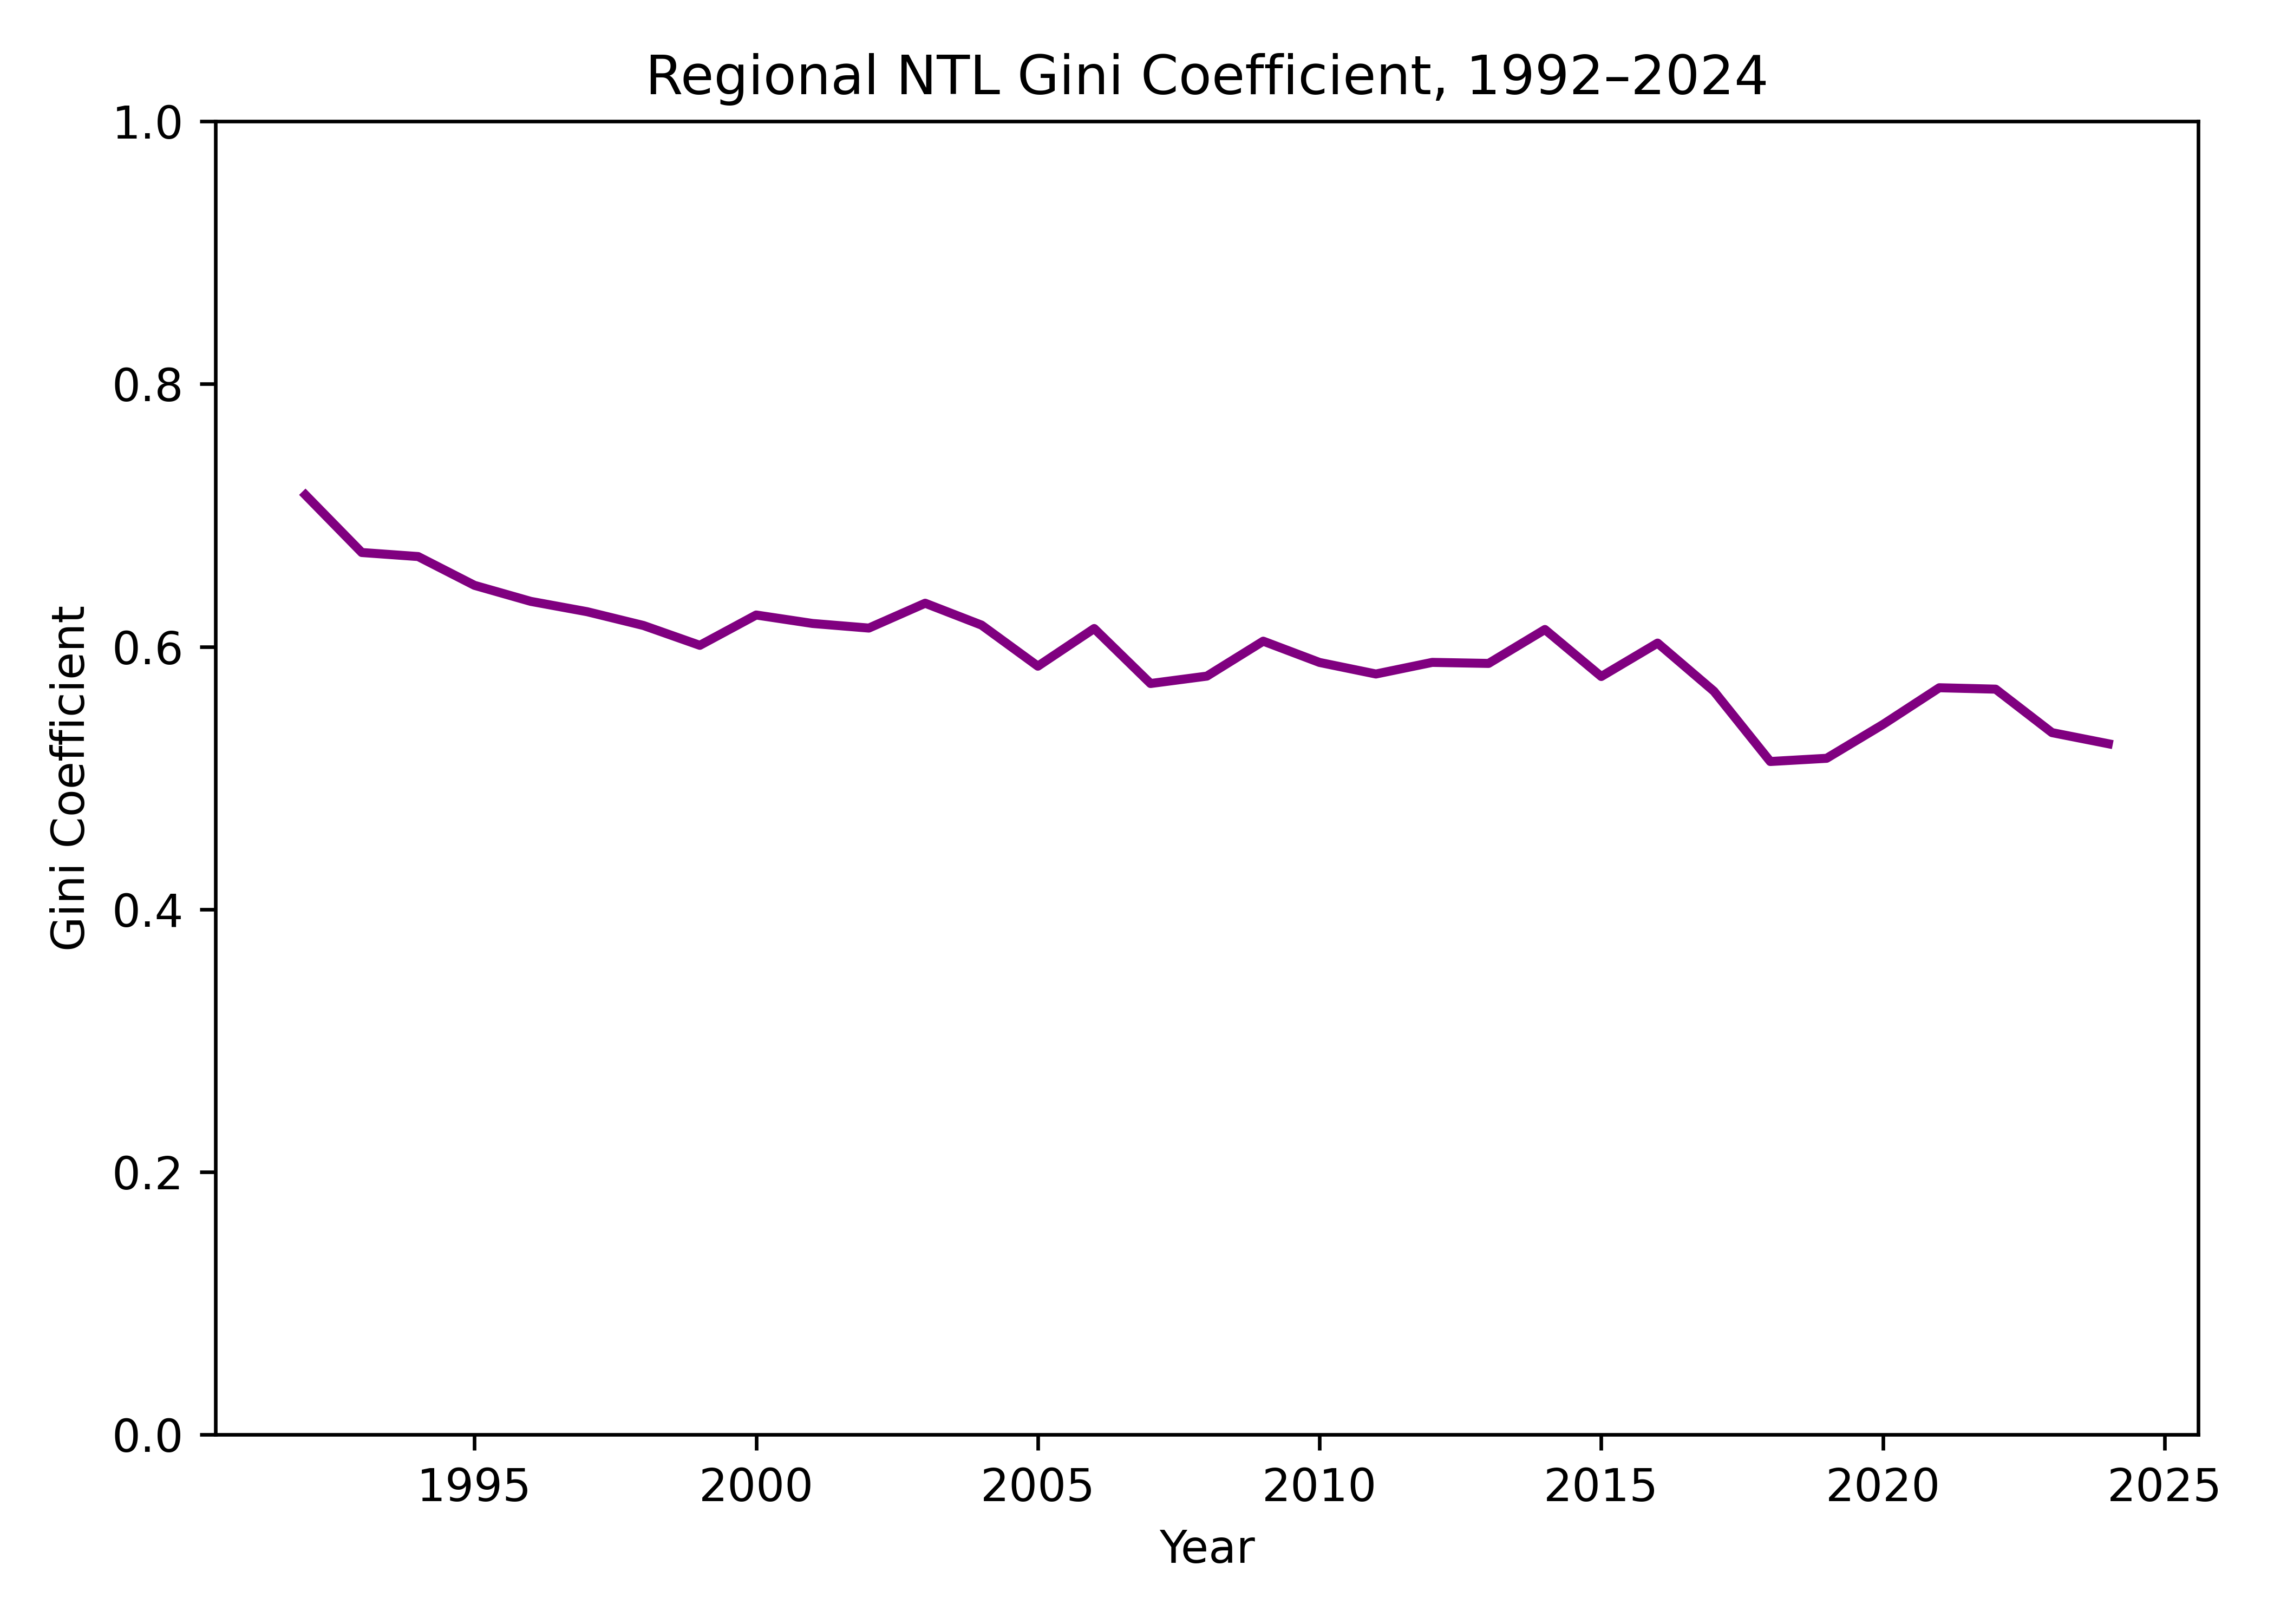
\includegraphics[width=0.8\textwidth]{outputs/figures/regional/regional_ntl_gini_trend.png}
	\caption{Regional luminosity inequality in Ethiopia, 1992--2024. The Gini coefficient summarizes the distribution of nighttime lights across regions, showing a decline in inequality through 2018 and a partial rebound by 2024. This trend contextualizes the empirical analysis of favoritism and highlights the evolving spatial concentration of economic activity.}
	\label{fig:gini_fig}
\end{figure}
% --- End Figure 2 ---

% --- Begin Figure: NTL vs GDP Validation ---
\begin{figure}[ht]
	\centering
	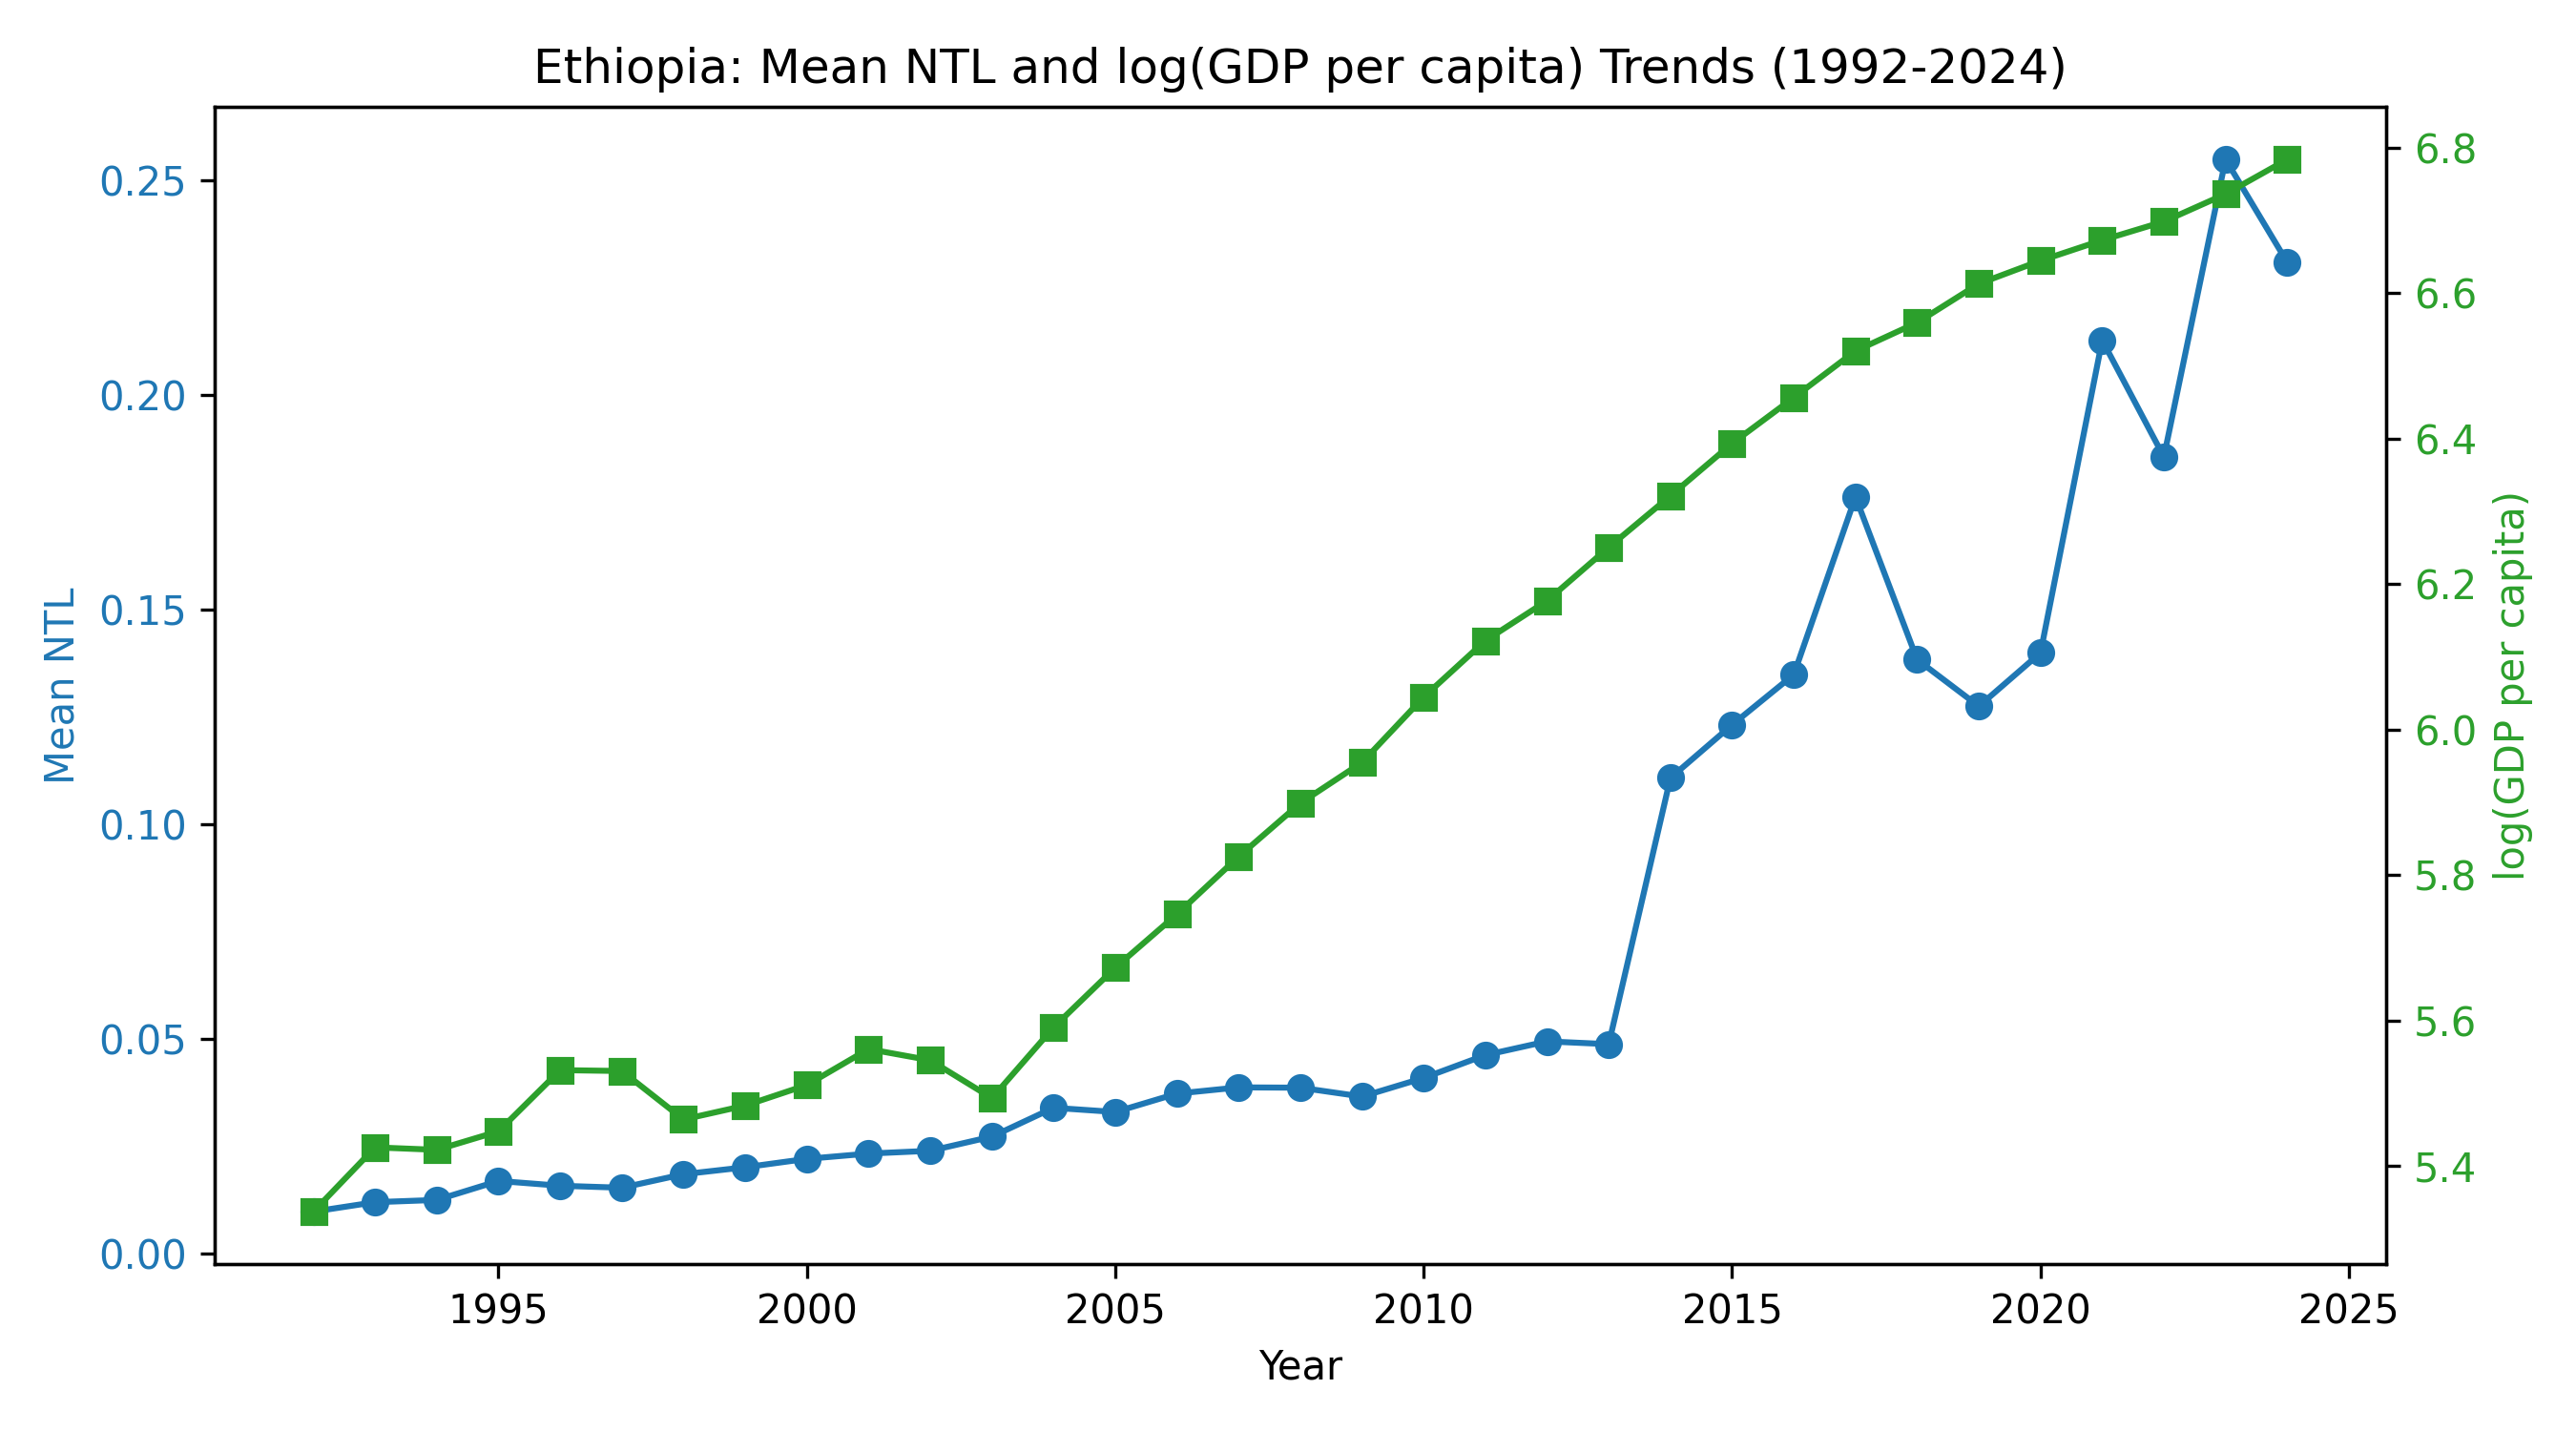
\includegraphics[width=0.7\textwidth]{outputs/figures/national/ntl_gdp_combined_trend.png}
	\caption{Validation of nighttime lights as a proxy for economic activity: National NTL and GDP per capita, 1992--2024. The strong comovement between NTL and GDP supports the use of satellite luminosity as a macroeconomic indicator in the Ethiopian context.}
	\label{fig:ntl_gdp_validation}
\end{figure}
% --- End Figure ---

This paper repositions the study of regional favoritism in political economy by exposing and explaining the systematic sources of bias in NTL-based empirical designs. The analysis demonstrates that sensitivity to specification is not a weakness of the data or methods per se, but rather a predictable outcome of three structural mechanisms. First, there is an urban and electrification bias embedded in NTL as a proxy for economic activity. In addition, the instability and ambiguity of regional administrative boundaries over time further complicate inference. Furthermore, the limited number of exogenous leadership transitions available for credible identification constrains the analysis. Existing literature has largely overlooked these mechanisms, often treating NTL-based favoritism estimates as robust to analytic choices and implicitly assuming that specification variation reflects noise rather than bias.

By rigorously unpacking these mechanisms, the present study demonstrates that much of the reported evidence for regional favoritism is an artifact of specification-driven bias, rather than a reflection of underlying political or economic processes. The contribution is affirmative: it provides a replicable framework for diagnosing and correcting specification sensitivity, and it sets a new empirical benchmark for studies leveraging remotely sensed data in political economy. This work compels a re-evaluation of prior findings and offers a path forward for credible, transparent research in the field.

\section{Literature Review}
This study sits at the intersection of three literatures.

First, a substantial literature uses satellite luminosity to measure economic activity. Early work established that light emissions track national and regional output surprisingly well in settings with limited conventional statistics \citep{Chen2011,Henderson2012}. More recent contributions show that the strength of this relationship varies with population density, sectoral composition, and spatial scale, which makes local interpretation more difficult than national validation exercises might suggest \citep{Bluhm2022,Gibson2021}. Work on harmonized long-run products has also improved the temporal comparability of DMSP-OLS and VIIRS series, but it has not eliminated measurement challenges \citep{Li2023,Gibson2024}.

Second, the paper relates to research on regional and ethnic favoritism. \citet{Hodler2014} show that political leaders' birth regions tend to receive higher nighttime light intensity in a broad cross-country sample. Subsequent work has refined that perspective by emphasizing the interaction between political favoritism, local ethnic demography, and institutions \citep{BeiserMcGrath2021}. Recent studies also continue to find geographically targeted favoritism in other settings, including public investment and local clientelism \citep{Onana2024,Cruzatti2024}. The implication is not that favoritism is universal, but that claims about it should be tested against within-unit changes rather than cross-sectional differences.




Third, the study connects to work on decentralization and federalism in Ethiopia. Existing scholarship highlights the tension between formal regional autonomy and persistent vertical control, including constraints on local fiscal autonomy and uneven developmental capacity \citep{Faguet2021,Wubneh2017}. Those institutional features make Ethiopia a theoretically important case for studying regional inequality, but they also heighten the need for careful empirical design. If regional trajectories differ for structural reasons unrelated to political leadership, pooled cross-sectional comparisons can easily be mistaken for favoritism.

\subsection*{Political Economy of Ethiopian Federalism}
The spatial distribution of rents in Ethiopia is deeply shaped by the country’s federal architecture and the political strategies of its ruling coalitions. Under the Ethiopian People’s Revolutionary Democratic Front (EPRDF), federalism was formally enshrined, but real power remained highly centralized. The EPRDF’s dominance over regional governments meant that resource allocation, investment, and development projects were often coordinated from the center, with regional administrations acting as agents rather than autonomous principals. This centralization is theorized to produce a spatial distribution of rents that is less responsive to local political dynamics and more reflective of national priorities and coalition management. In contrast, the current administration has presided over a period of greater regional contestation and, in some cases, increased regional autonomy. According to \citet{Faguet2021}, such shifts can alter the expected pattern of rent distribution: as regional governments gain more effective autonomy, the allocation of resources may become more sensitive to local political competition, ethnic demography, and the bargaining power of regional elites. This theoretical perspective suggests that the empirical analysis of favoritism in Ethiopia must account for changes in the structure of federalism and the evolving balance of power between center and regions.

Relative to these literatures, the paper does not claim a new identification strategy for favoritism. Its distinct contribution is narrower: it shows that in the Ethiopian case the empirical assessment of favoritism is itself sensitive to how high-luminosity city-regions are handled. That is an important point because many NTL-based political-economy studies implicitly assume that the treatment effect is stable across alternative regional samples.

\section{Methodology}
\subsection{Data}
\subsubsection{Nighttime light data}
The repository contains a harmonized annual NTL series built from DMSP-OLS and VIIRS raster products. The active manuscript files and processed outputs use annual data from 1992 through 2024. The underlying scripts reference the pixel-scale corrected nighttime light product of \citet{Li2023} and annual VIIRS composites derived by \citet{Elvidge2021}. Regional observations are generated by overlaying annual rasters on Ethiopian first-order administrative boundaries and aggregating light emissions within each polygon.

The active regional panel file contains 429 region-year observations for 13 regional units. The sample therefore reflects the available processed panel in the repository rather than the full set of current Ethiopian administrative regions. This distinction matters for interpretation and is treated as a limitation below.
% --- Begin Figure 5: Admin Map ---
\begin{figure}[ht]
	\centering
	% Replace the following line with the actual path to your admin map graphic
	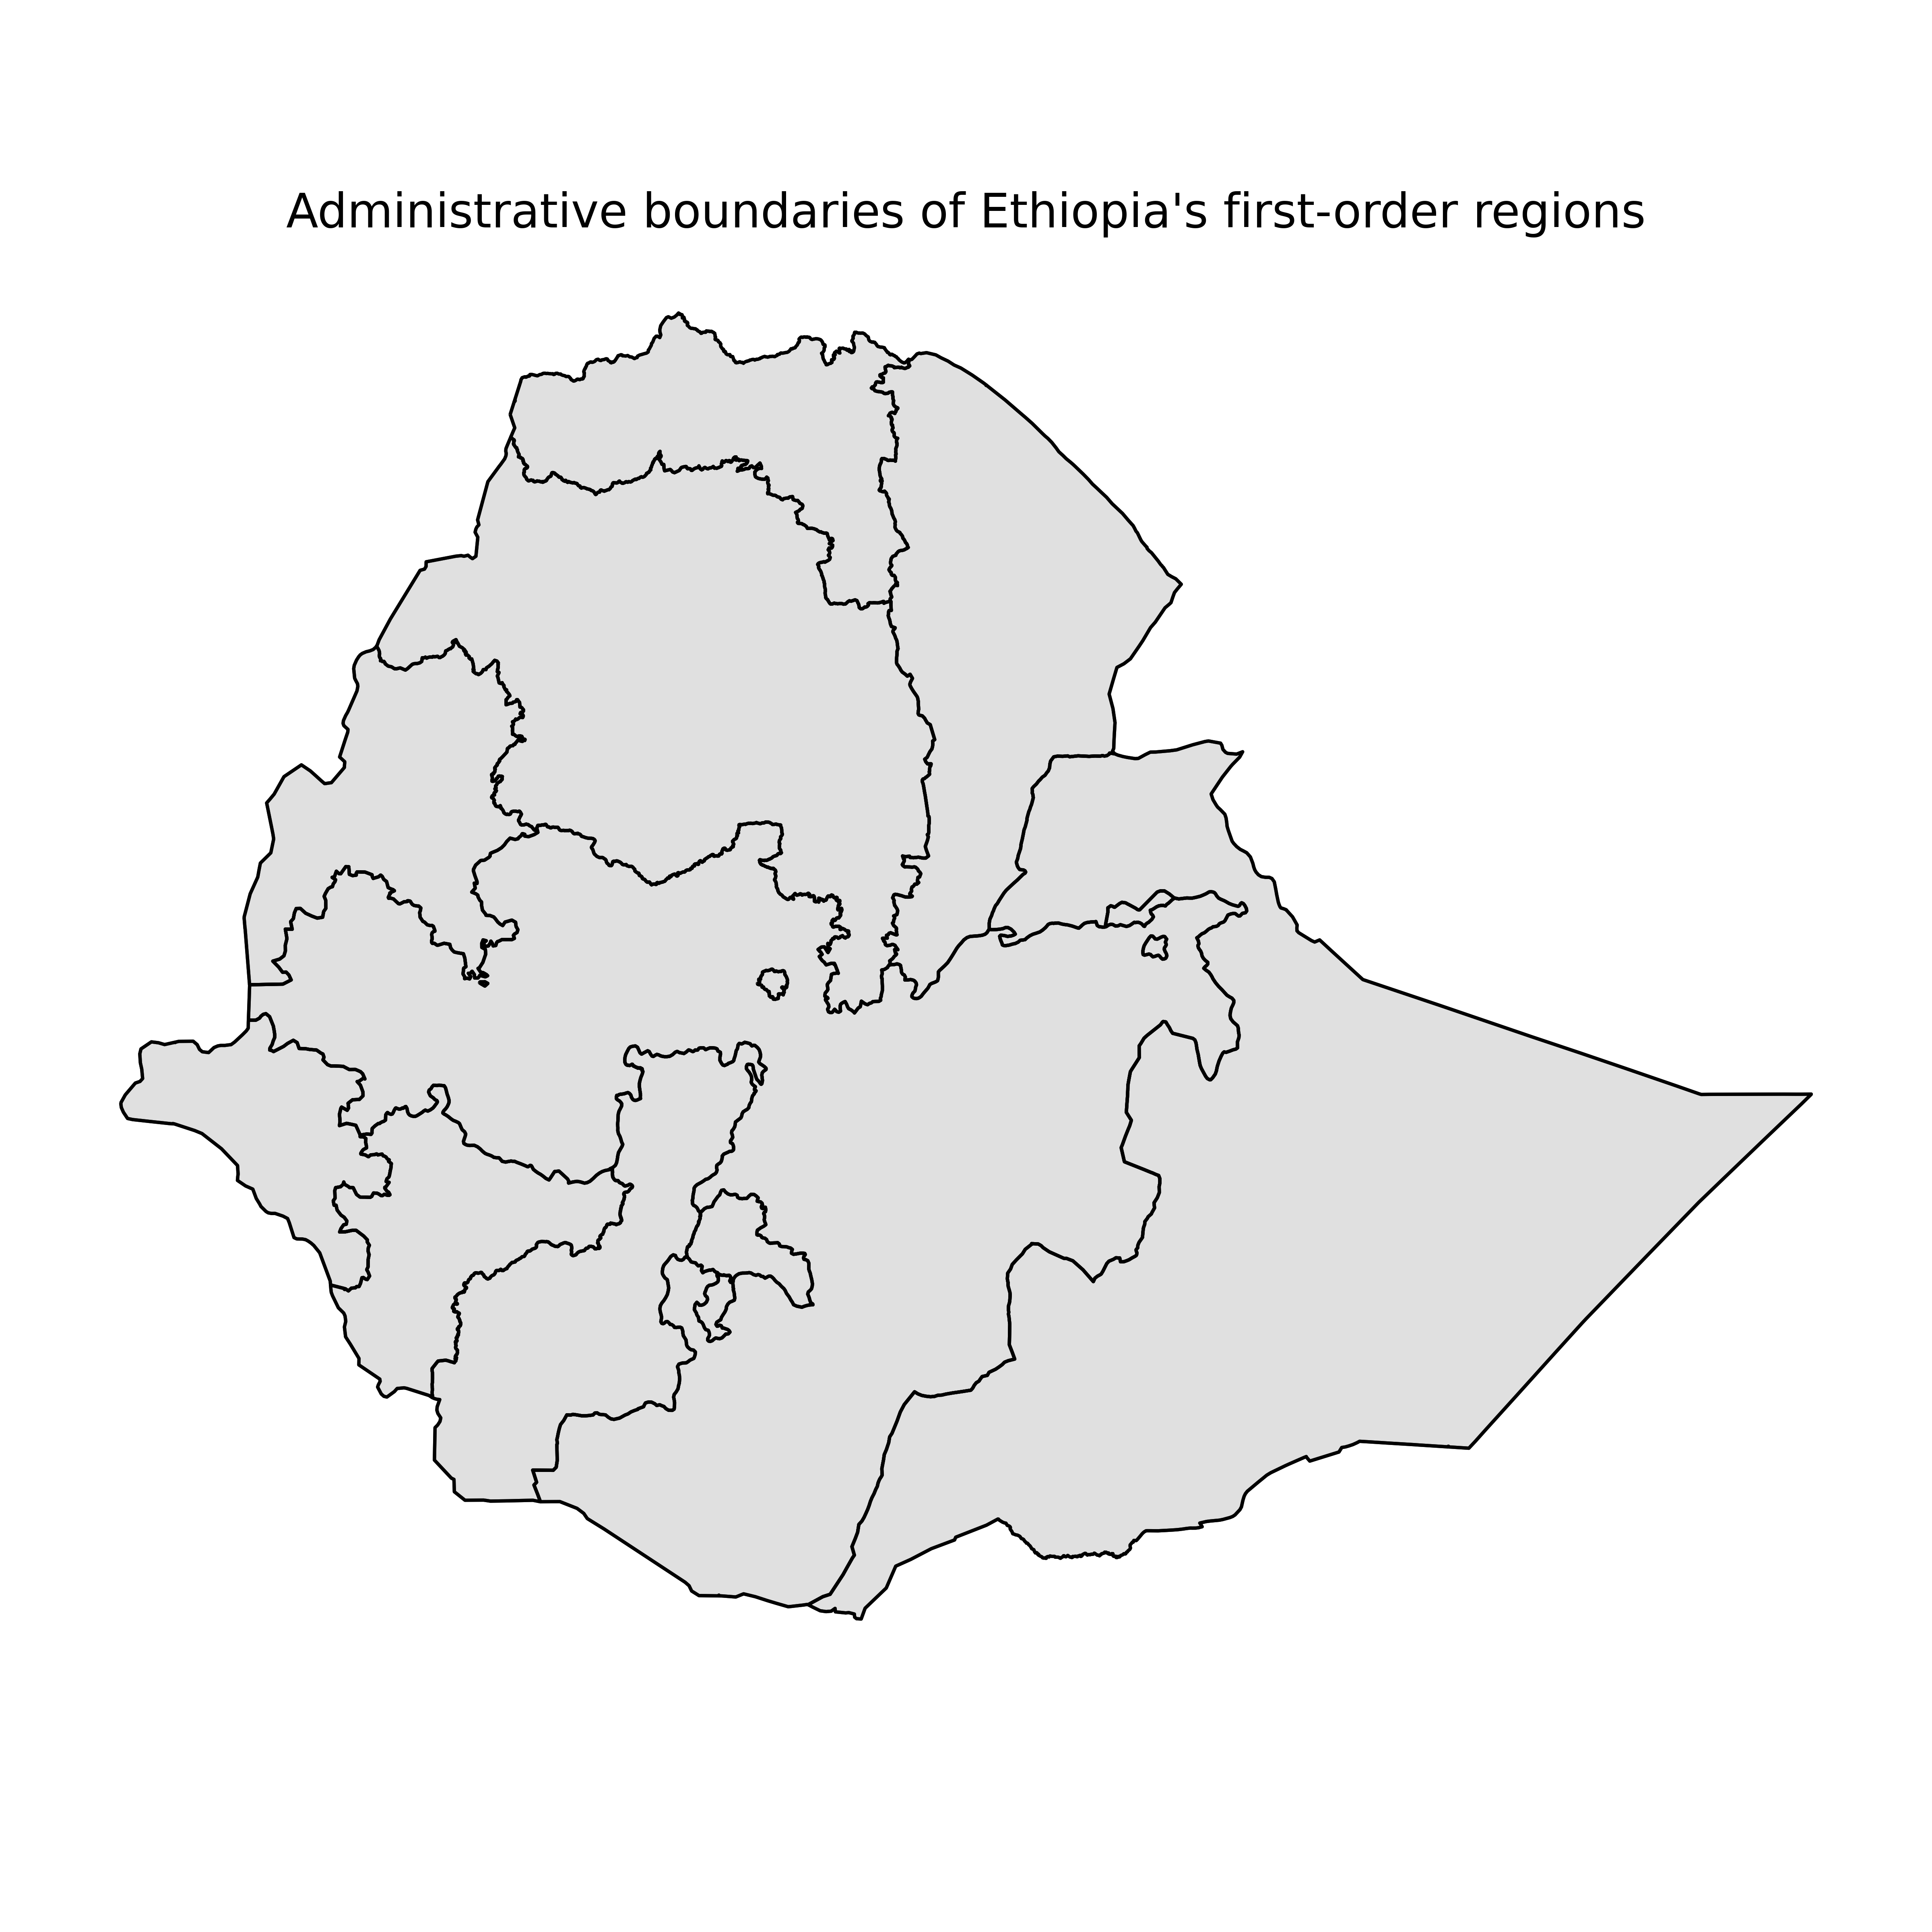
\includegraphics[width=0.7\textwidth]{outputs/figures/admin/ethiopia_admin_map.png}
	\caption{Administrative boundaries of Ethiopia's first-order regions. The map displays the 13 regional units used in the analysis, highlighting the evolving and fragmented nature of administrative boundaries over the study period.}
	\label{fig:admin_map}
\end{figure}
% --- End Figure 5 ---

\section{Identification Challenges in Small-N Panel Settings}

In empirical analyses of political favoritism using nighttime lights (NTL) data, identification is particularly challenging in settings with a small number of regions, limited exogenous variation in treatment, and high outcome concentration. This section outlines three core challenges that jointly limit inference in such panel data contexts.

\subsection{Omitted Variable Bias (without time fixed effects)}

When time fixed effects are omitted from panel regressions, estimates of leader-region favoritism are vulnerable to omitted variable bias. In the Ethiopian context, national economic shocks—such as booms or downturns—often coincide with leadership transitions. Without controlling for year effects, the estimated association between a leader’s birth region and regional luminosity may simply reflect these broader national trends, rather than any causal effect of political favoritism. Empirically, baseline models that exclude time fixed effects tend to produce inflated and statistically significant coefficients, but placebo tests and diagnostic plots reveal that these results are largely driven by common shocks rather than genuine treatment effects.

\subsection{Limited Identifying Variation (with time fixed effects)}

Including time fixed effects absorbs national shocks and common trends, but in small-N settings with few treated units and limited within-region, within-year variation, this approach introduces a new problem: limited identifying variation. When the timing of leader transitions is highly collinear with year effects, the model cannot reliably distinguish leader-region effects from national shocks. In the Ethiopian panel, the inclusion of time fixed effects sharply attenuates the estimated coefficients and increases standard errors, indicating that the available variation is insufficient for robust identification. The empirical p-values from placebo tests further confirm that observed effects are not distinguishable from random assignment.

\subsection{Low Statistical Power (small number of treated units)}

A third challenge is low statistical power, which arises from the small number of regions and limited number of leadership transitions. With only a handful of treated units and sparse treatment events, the effective sample size for identifying leader-region effects is severely constrained. This results in wide confidence intervals and imprecise estimates, particularly in event-study analyses and placebo simulations. The inability to detect dynamic effects or distinguish real from placebo results is a direct consequence of this low power, as demonstrated by the high empirical p-values and the overlap between observed and placebo distributions.

\paragraph{Synthesis}

Taken together, these challenges—omitted variable bias, limited identifying variation, and low statistical power—jointly undermine the credibility of causal inference in small-N panel settings. In the Ethiopian case, and in similar contexts, the combination of these factors means that apparent evidence for political favoritism is not empirically distinguishable from noise. Robust identification requires richer data, more exogenous variation, and careful diagnostic testing to avoid spurious findings.

\section{Literature Review}
This study sits at the intersection of three literatures.

First, a substantial literature uses satellite luminosity to measure economic activity. Early work established that light emissions track national and regional output surprisingly well in settings with limited conventional statistics \citep{Chen2011,Henderson2012}. More recent contributions show that the strength of this relationship varies with population density, sectoral composition, and spatial scale, which makes local interpretation more difficult than national validation exercises might suggest \citep{Bluhm2022,Gibson2021}. Work on harmonized long-run products has also improved the temporal comparability of DMSP-OLS and VIIRS series, but it has not eliminated measurement challenges \citep{Li2023,Gibson2024}.

Second, the paper relates to research on regional and ethnic favoritism. \citet{Hodler2014} show that political leaders' birth regions tend to receive higher nighttime light intensity in a broad cross-country sample. Subsequent work has refined that perspective by emphasizing the interaction between political favoritism, local ethnic demography, and institutions \citep{BeiserMcGrath2021}. Recent studies also continue to find geographically targeted favoritism in other settings, including public investment and local clientelism \citep{Onana2024,Cruzatti2024}. The implication is not that favoritism is universal, but that claims about it should be tested against within-unit changes rather than cross-sectional differences.




Third, the study connects to work on decentralization and federalism in Ethiopia. Existing scholarship highlights the tension between formal regional autonomy and persistent vertical control, including constraints on local fiscal autonomy and uneven developmental capacity \citep{Faguet2021,Wubneh2017}. Those institutional features make Ethiopia a theoretically important case for studying regional inequality, but they also heighten the need for careful empirical design. If regional trajectories differ for structural reasons unrelated to political leadership, pooled cross-sectional comparisons can easily be mistaken for favoritism.

\subsection*{Political Economy of Ethiopian Federalism}
The spatial distribution of rents in Ethiopia is deeply shaped by the country’s federal architecture and the political strategies of its ruling coalitions. Under the Ethiopian People’s Revolutionary Democratic Front (EPRDF), federalism was formally enshrined, but real power remained highly centralized. The EPRDF’s dominance over regional governments meant that resource allocation, investment, and development projects were often coordinated from the center, with regional administrations acting as agents rather than autonomous principals. This centralization is theorized to produce a spatial distribution of rents that is less responsive to local political dynamics and more reflective of national priorities and coalition management. In contrast, the current administration has presided over a period of greater regional contestation and, in some cases, increased regional autonomy. According to \citet{Faguet2021}, such shifts can alter the expected pattern of rent distribution: as regional governments gain more effective autonomy, the allocation of resources may become more sensitive to local political competition, ethnic demography, and the bargaining power of regional elites. This theoretical perspective suggests that the empirical analysis of favoritism in Ethiopia must account for changes in the structure of federalism and the evolving balance of power between center and regions.

Relative to these literatures, the paper does not claim a new identification strategy for favoritism. Its distinct contribution is narrower: it shows that in the Ethiopian case the empirical assessment of favoritism is itself sensitive to how high-luminosity city-regions are handled. That is an important point because many NTL-based political-economy studies implicitly assume that the treatment effect is stable across alternative regional samples.

\section{Methodology}
\subsection{Data}
\subsubsection{Nighttime light data}
The repository contains a harmonized annual NTL series built from DMSP-OLS and VIIRS raster products. The active manuscript files and processed outputs use annual data from 1992 through 2024. The underlying scripts reference the pixel-scale corrected nighttime light product of \citet{Li2023} and annual VIIRS composites derived by \citet{Elvidge2021}. Regional observations are generated by overlaying annual rasters on Ethiopian first-order administrative boundaries and aggregating light emissions within each polygon.

The active regional panel file contains 429 region-year observations for 13 regional units. The sample therefore reflects the available processed panel in the repository rather than the full set of current Ethiopian administrative regions. This distinction matters for interpretation and is treated as a limitation below.
% --- Begin Figure 5: Admin Map ---
\begin{figure}[ht]
	\centering
	% Replace the following line with the actual path to your admin map graphic
	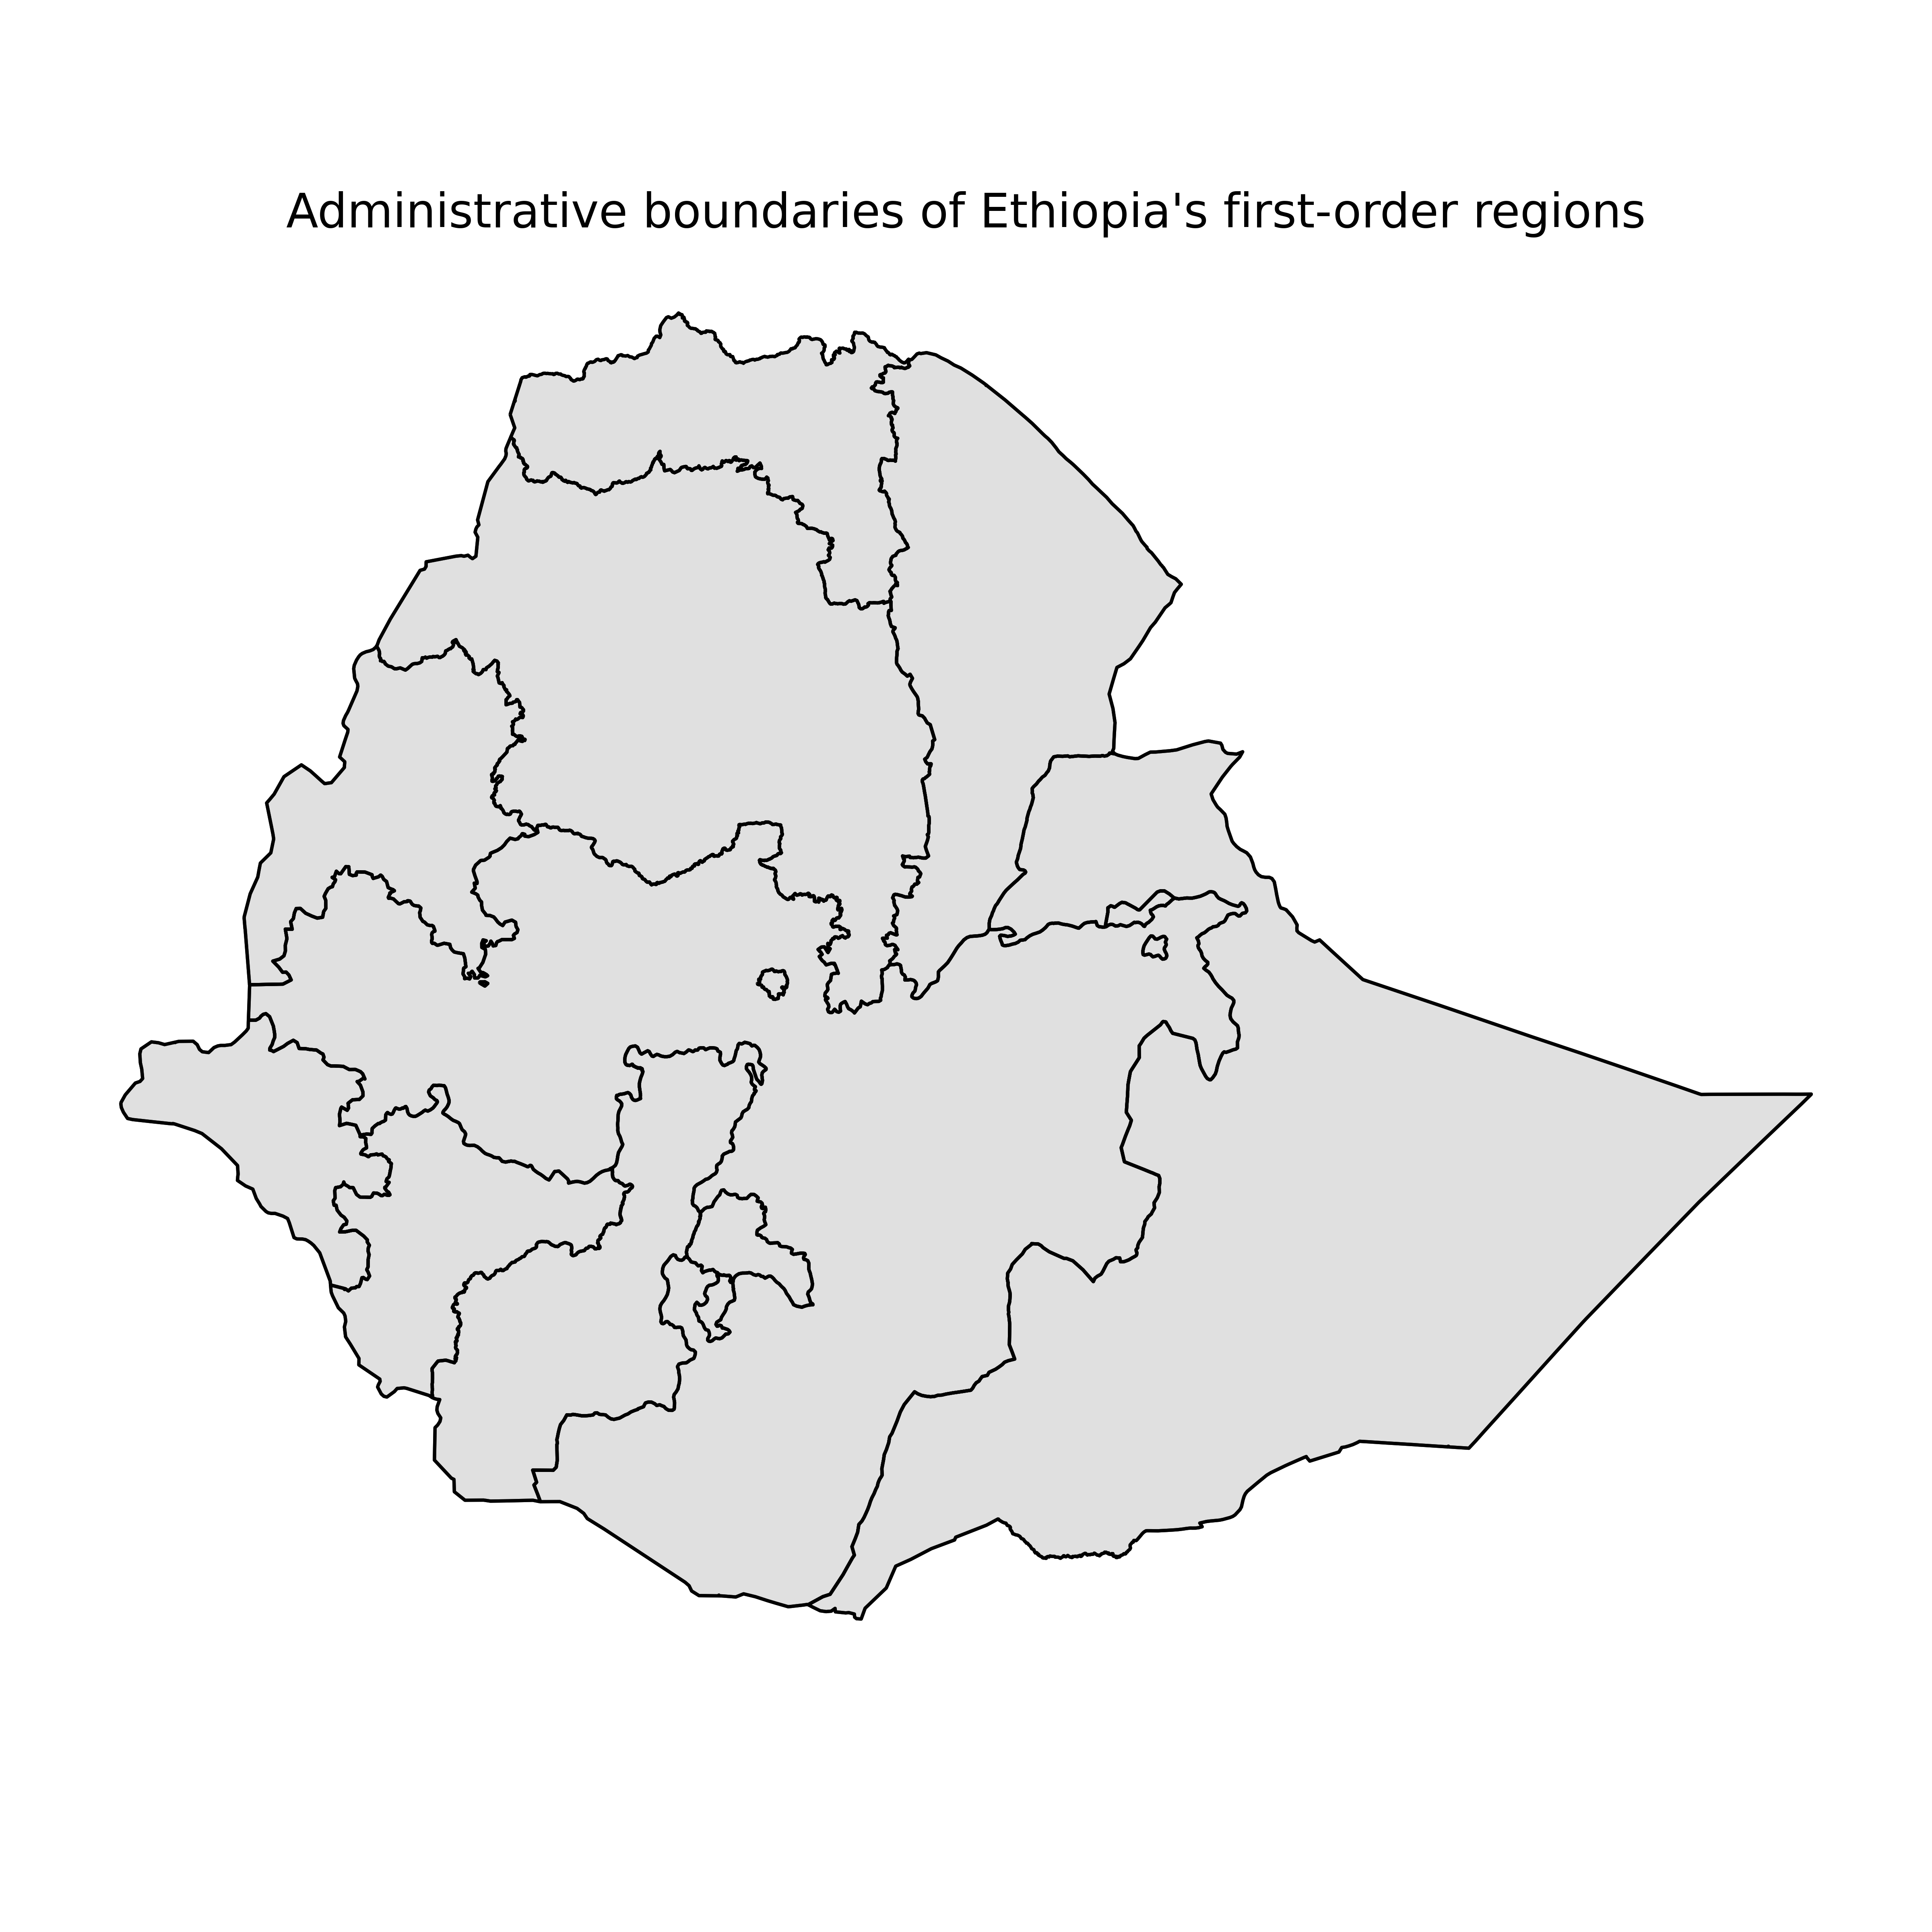
\includegraphics[width=0.7\textwidth]{outputs/figures/admin/ethiopia_admin_map.png}
	\caption{Administrative boundaries of Ethiopia's first-order regions. The map displays the 13 regional units used in the analysis, highlighting the evolving and fragmented nature of administrative boundaries over the study period.}
	\label{fig:admin_map}
\end{figure}
% --- End Figure 5 ---

\section{Identification Challenges in Small-N Panel Settings}

In empirical analyses of political favoritism using nighttime lights (NTL) data, identification is particularly challenging in settings with a small number of regions, limited exogenous variation in treatment, and high outcome concentration. This section outlines three core challenges that jointly limit inference in such panel data contexts.

\subsection{Omitted Variable Bias (without time fixed effects)}

When time fixed effects are omitted from panel regressions, estimates of leader-region favoritism are vulnerable to omitted variable bias. In the Ethiopian context, national economic shocks—such as booms or downturns—often coincide with leadership transitions. Without controlling for year effects, the estimated association between a leader’s birth region and regional luminosity may simply reflect these broader national trends, rather than any causal effect of political favoritism. Empirically, baseline models that exclude time fixed effects tend to produce inflated and statistically significant coefficients, but placebo tests and diagnostic plots reveal that these results are largely driven by common shocks rather than genuine treatment effects.

\subsection{Limited Identifying Variation (with time fixed effects)}

Including time fixed effects absorbs national shocks and common trends, but in small-N settings with few treated units and limited within-region, within-year variation, this approach introduces a new problem: limited identifying variation. When the timing of leader transitions is highly collinear with year effects, the model cannot reliably distinguish leader-region effects from national shocks. In the Ethiopian panel, the inclusion of time fixed effects sharply attenuates the estimated coefficients and increases standard errors, indicating that the available variation is insufficient for robust identification. The empirical p-values from placebo tests further confirm that observed effects are not distinguishable from random assignment.

\subsection{Low Statistical Power (small number of treated units)}

A third challenge is low statistical power, which arises from the small number of regions and limited number of leadership transitions. With only a handful of treated units and sparse treatment events, the effective sample size for identifying leader-region effects is severely constrained. This results in wide confidence intervals and imprecise estimates, particularly in event-study analyses and placebo simulations. The inability to detect dynamic effects or distinguish real from placebo results is a direct consequence of this low power, as demonstrated by the high empirical p-values and the overlap between observed and placebo distributions.

\paragraph{Synthesis}

Taken together, these challenges—omitted variable bias, limited identifying variation, and low statistical power—jointly undermine the credibility of causal inference in small-N panel settings. In the Ethiopian case, and in similar contexts, the combination of these factors means that apparent evidence for political favoritism is not empirically distinguishable from noise. Robust identification requires richer data, more exogenous variation, and careful diagnostic testing to avoid spurious findings.

\section{Literature Review}
This study sits at the intersection of three literatures.

First, a substantial literature uses satellite luminosity to measure economic activity. Early work established that light emissions track national and regional output surprisingly well in settings with limited conventional statistics \citep{Chen2011,Henderson2012}. More recent contributions show that the strength of this relationship varies with population density, sectoral composition, and spatial scale, which makes local interpretation more difficult than national validation exercises might suggest \citep{Bluhm2022,Gibson2021}. Work on harmonized long-run products has also improved the temporal comparability of DMSP-OLS and VIIRS series, but it has not eliminated measurement challenges \citep{Li2023,Gibson2024}.

Second, the paper relates to research on regional and ethnic favoritism. \citet{Hodler2014} show that political leaders' birth regions tend to receive higher nighttime light intensity in a broad cross-country sample. Subsequent work has refined that perspective by emphasizing the interaction between political favoritism, local ethnic demography, and institutions \citep{BeiserMcGrath2021}. Recent studies also continue to find geographically targeted favoritism in other settings, including public investment and local clientelism \citep{Onana2024,Cruzatti2024}. The implication is not that favoritism is universal, but that claims about it should be tested against within-unit changes rather than cross-sectional differences.




Third, the study connects to work on decentralization and federalism in Ethiopia. Existing scholarship highlights the tension between formal regional autonomy and persistent vertical control, including constraints on local fiscal autonomy and uneven developmental capacity \citep{Faguet2021,Wubneh2017}. Those institutional features make Ethiopia a theoretically important case for studying regional inequality, but they also heighten the need for careful empirical design. If regional trajectories differ for structural reasons unrelated to political leadership, pooled cross-sectional comparisons can easily be mistaken for favoritism.

\subsection*{Political Economy of Ethiopian Federalism}
The spatial distribution of rents in Ethiopia is deeply shaped by the country’s federal architecture and the political strategies of its ruling coalitions. Under the Ethiopian People’s Revolutionary Democratic Front (EPRDF), federalism was formally enshrined, but real power remained highly centralized. The EPRDF’s dominance over regional governments meant that resource allocation, investment, and development projects were often coordinated from the center, with regional administrations acting as agents rather than autonomous principals. This centralization is theorized to produce a spatial distribution of rents that is less responsive to local political dynamics and more reflective of national priorities and coalition management. In contrast, the current administration has presided over a period of greater regional contestation and, in some cases, increased regional autonomy. According to \citet{Faguet2021}, such shifts can alter the expected pattern of rent distribution: as regional governments gain more effective autonomy, the allocation of resources may become more sensitive to local political competition, ethnic demography, and the bargaining power of regional elites. This theoretical perspective suggests that the empirical analysis of favoritism in Ethiopia must account for changes in the structure of federalism and the evolving balance of power between center and regions.

Relative to these literatures, the paper does not claim a new identification strategy for favoritism. Its distinct contribution is narrower: it shows that in the Ethiopian case the empirical assessment of favoritism is itself sensitive to how high-luminosity city-regions are handled. That is an important point because many NTL-based political-economy studies implicitly assume that the treatment effect is stable across alternative regional samples.

\section{Methodology}
\subsection{Data}
\subsubsection{Nighttime light data}
The repository contains a harmonized annual NTL series built from DMSP-OLS and VIIRS raster products. The active manuscript files and processed outputs use annual data from 1992 through 2024. The underlying scripts reference the pixel-scale corrected nighttime light product of \citet{Li2023} and annual VIIRS composites derived by \citet{Elvidge2021}. Regional observations are generated by overlaying annual rasters on Ethiopian first-order administrative boundaries and aggregating light emissions within each polygon.

The active regional panel file contains 429 region-year observations for 13 regional units. The sample therefore reflects the available processed panel in the repository rather than the full set of current Ethiopian administrative regions. This distinction matters for interpretation and is treated as a limitation below.
% --- Begin Figure 5: Admin Map ---
\begin{figure}[ht]
	\centering
	% Replace the following line with the actual path to your admin map graphic
	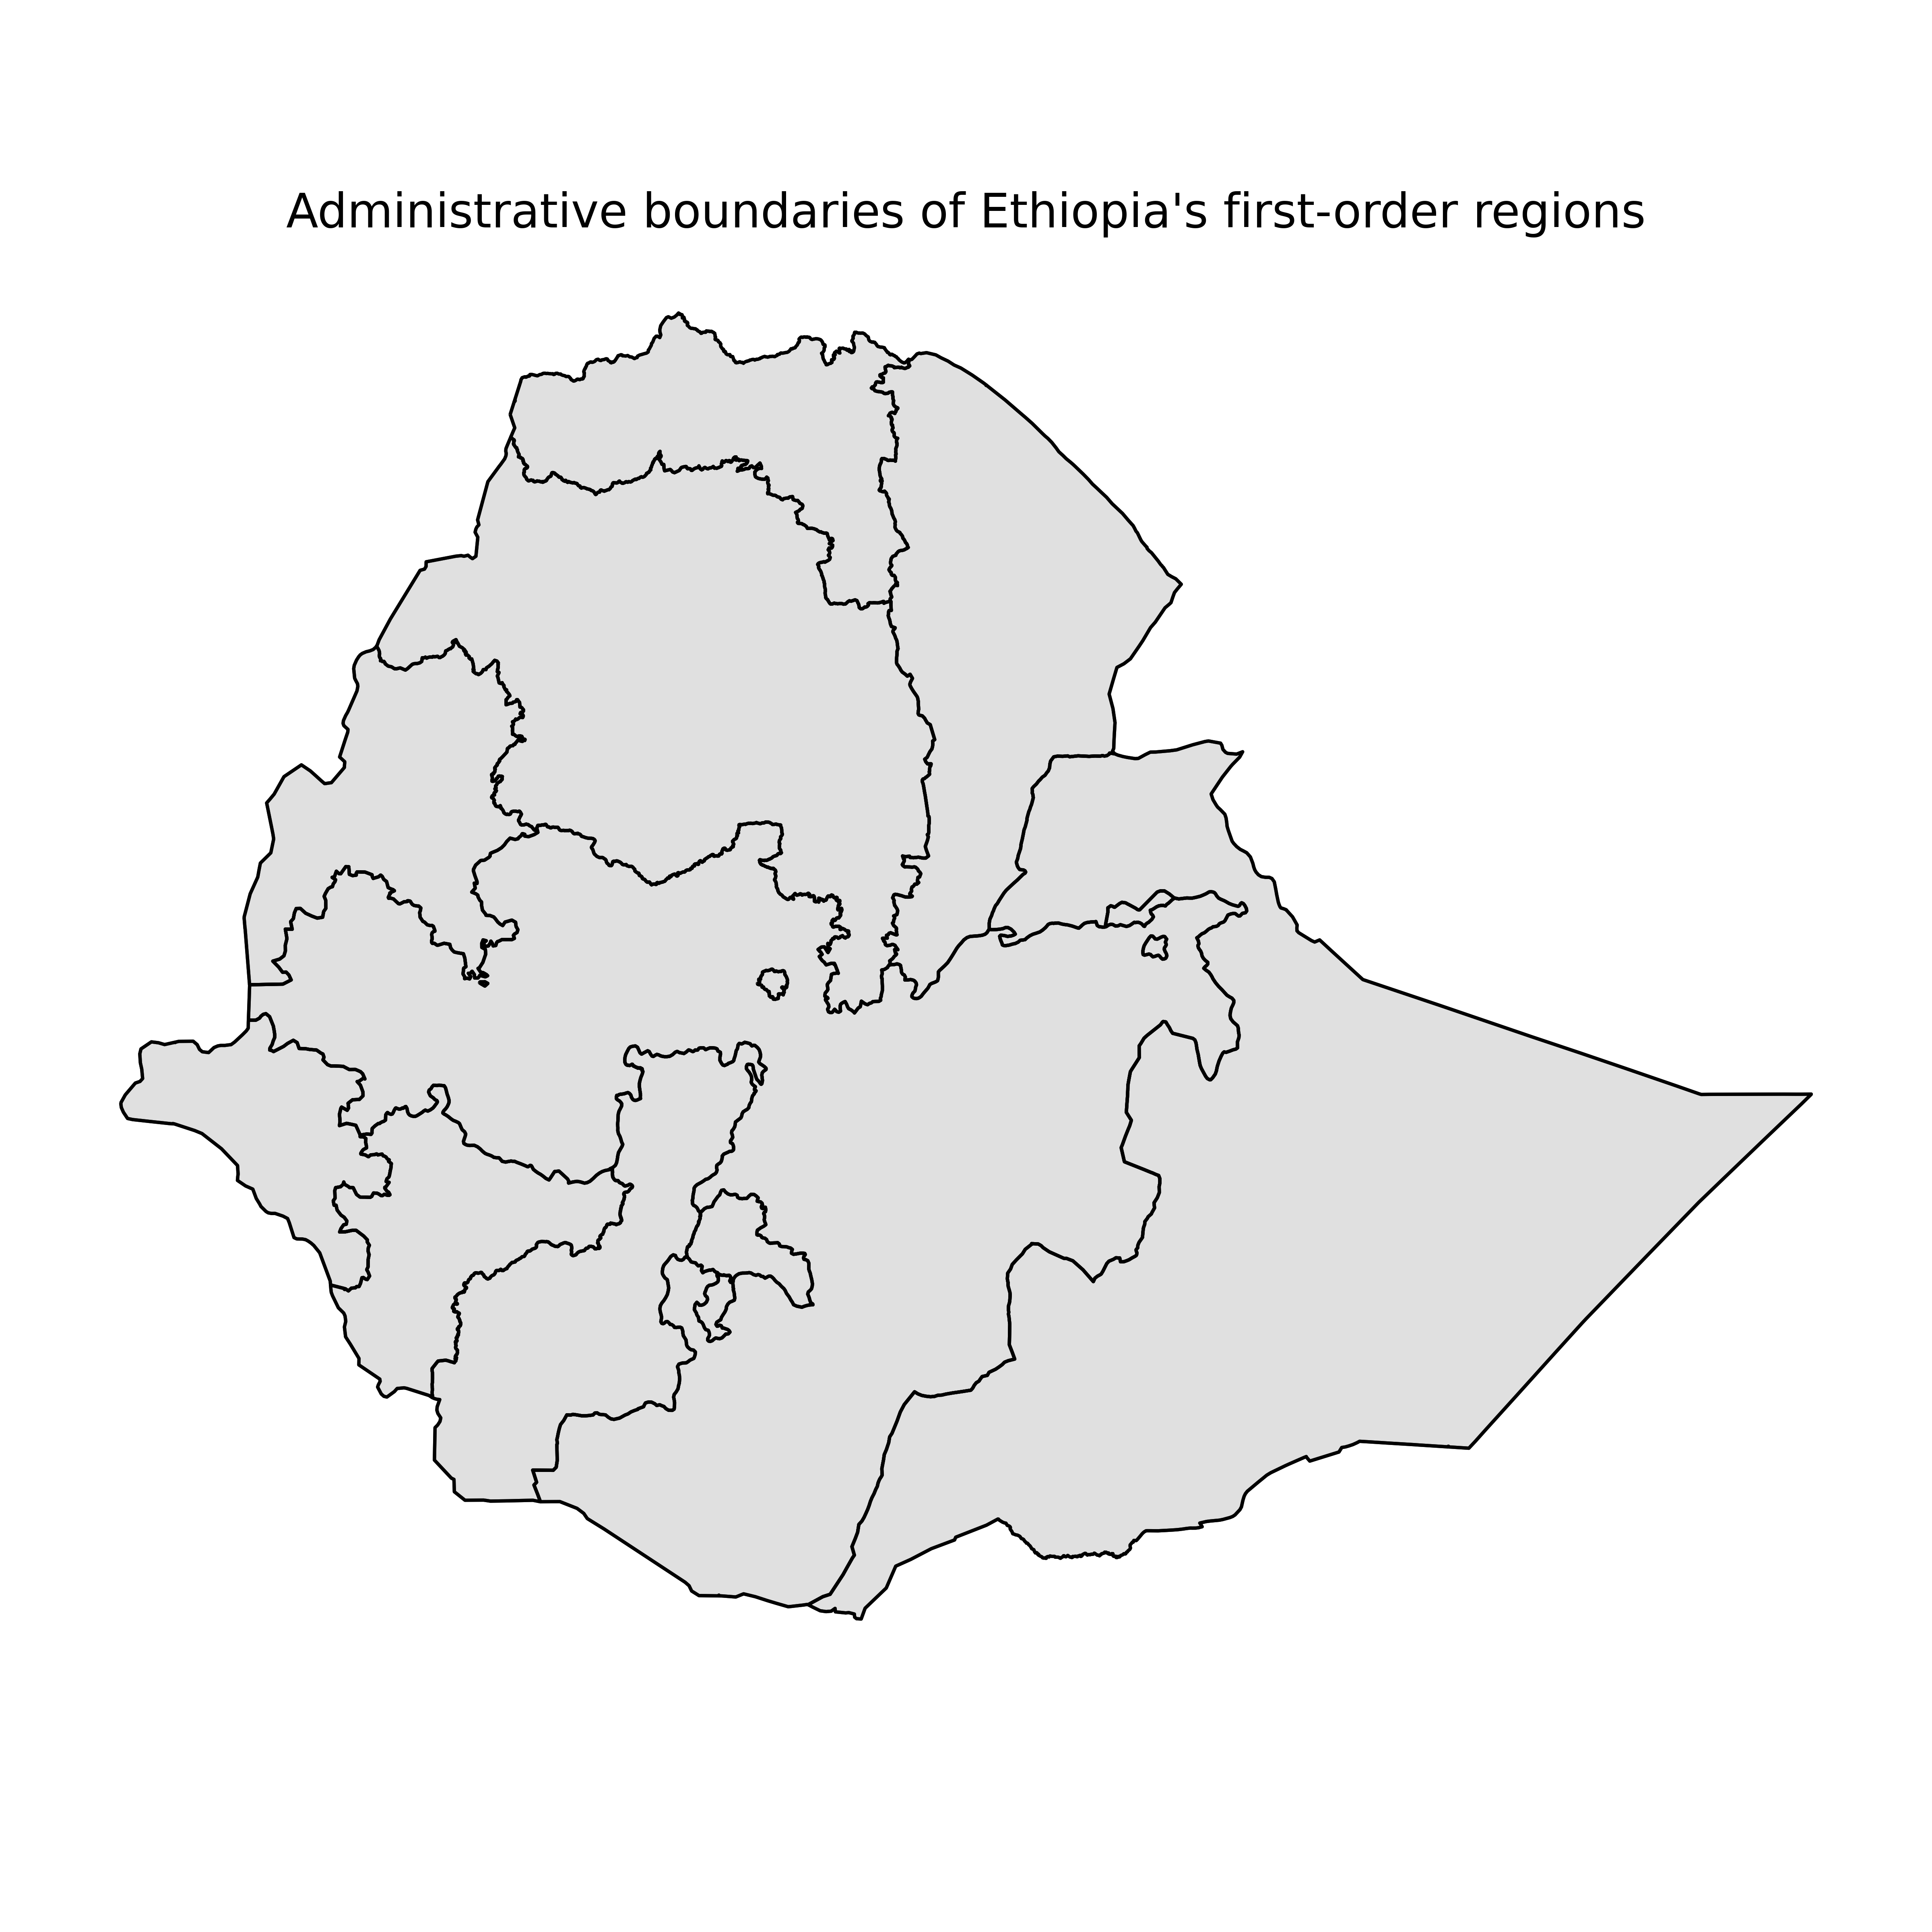
\includegraphics[width=0.7\textwidth]{outputs/figures/admin/ethiopia_admin_map.png}
	\caption{Administrative boundaries of Ethiopia's first-order regions. The map displays the 13 regional units used in the analysis, highlighting the evolving and fragmented nature of administrative boundaries over the study period.}
	\label{fig:admin_map}
\end{figure}
% --- End Figure 5 ---

\section{Identification Challenges in Small-N Panel Settings}

In empirical analyses of political favoritism using nighttime lights (NTL) data, identification is particularly challenging in settings with a small number of regions, limited exogenous variation in treatment, and high outcome concentration. This section outlines three core challenges that jointly limit inference in such panel data contexts.

\subsection{Omitted Variable Bias (without time fixed effects)}

When time fixed effects are omitted from panel regressions, estimates of leader-region favoritism are vulnerable to omitted variable bias. In the Ethiopian context, national economic shocks—such as booms or downturns—often coincide with leadership transitions. Without controlling for year effects, the estimated association between a leader’s birth region and regional luminosity may simply reflect these broader national trends, rather than any causal effect of political favoritism. Empirically, baseline models that exclude time fixed effects tend to produce inflated and statistically significant coefficients, but placebo tests and diagnostic plots reveal that these results are largely driven by common shocks rather than genuine treatment effects.

\subsection{Limited Identifying Variation (with time fixed effects)}

Including time fixed effects absorbs national shocks and common trends, but in small-N settings with few treated units and limited within-region, within-year variation, this approach introduces a new problem: limited identifying variation. When the timing of leader transitions is highly collinear with year effects, the model cannot reliably distinguish leader-region effects from national shocks. In the Ethiopian panel, the inclusion of time fixed effects sharply attenuates the estimated coefficients and increases standard errors, indicating that the available variation is insufficient for robust identification. The empirical p-values from placebo tests further confirm that observed effects are not distinguishable from random assignment.

\subsection{Low Statistical Power (small number of treated units)}

A third challenge is low statistical power, which arises from the small number of regions and limited number of leadership transitions. With only a handful of treated units and sparse treatment events, the effective sample size for identifying leader-region effects is severely constrained. This results in wide confidence intervals and imprecise estimates, particularly in event-study analyses and placebo simulations. The inability to detect dynamic effects or distinguish real from placebo results is a direct consequence of this low power, as demonstrated by the high empirical p-values and the overlap between observed and placebo distributions.

\paragraph{Synthesis}

Taken together, these challenges—omitted variable bias, limited identifying variation, and low statistical power—jointly undermine the credibility of causal inference in small-N panel settings. In the Ethiopian case, and in similar contexts, the combination of these factors means that apparent evidence for political favoritism is not empirically distinguishable from noise. Robust identification requires richer data, more exogenous variation, and careful diagnostic testing to avoid spurious findings.

\section{Literature Review}
This study sits at the intersection of three literatures.

First, a substantial literature uses satellite luminosity to measure economic activity. Early work established that light emissions track national and regional output surprisingly well in settings with limited conventional statistics \citep{Chen2011,Henderson2012}. More recent contributions show that the strength of this relationship varies with population density, sectoral composition, and spatial scale, which makes local interpretation more difficult than national validation exercises might suggest \citep{Bluhm2022,Gibson2021}. Work on harmonized long-run products has also improved the temporal comparability of DMSP-OLS and VIIRS series, but it has not eliminated measurement challenges \citep{Li2023,Gibson2024}.

Second, the paper relates to research on regional and ethnic favoritism. \citet{Hodler2014} show that political leaders' birth regions tend to receive higher nighttime light intensity in a broad cross-country sample. Subsequent work has refined that perspective by emphasizing the interaction between political favoritism, local ethnic demography, and institutions \citep{BeiserMcGrath2021}. Recent studies also continue to find geographically targeted favoritism in other settings, including public investment and local clientelism \citep{Onana2024,Cruzatti2024}. The implication is not that favoritism is universal, but that claims about it should be tested against within-unit changes rather than cross-sectional differences.




Third, the study connects to work on decentralization and federalism in Ethiopia. Existing scholarship highlights the tension between formal regional autonomy and persistent vertical control, including constraints on local fiscal autonomy and uneven developmental capacity \citep{Faguet2021,Wubneh2017}. Those institutional features make Ethiopia a theoretically important case for studying regional inequality, but they also heighten the need for careful empirical design. If regional trajectories differ for structural reasons unrelated to political leadership, pooled cross-sectional comparisons can easily be mistaken for favoritism.

\subsection*{Political Economy of Ethiopian Federalism}
The spatial distribution of rents in Ethiopia is deeply shaped by the country’s federal architecture and the political strategies of its ruling coalitions. Under the Ethiopian People’s Revolutionary Democratic Front (EPRDF), federalism was formally enshrined, but real power remained highly centralized. The EPRDF’s dominance over regional governments meant that resource allocation, investment, and development projects were often coordinated from the center, with regional administrations acting as agents rather than autonomous principals. This centralization is theorized to produce a spatial distribution of rents that is less responsive to local political dynamics and more reflective of national priorities and coalition management. In contrast, the current administration has presided over a period of greater regional contestation and, in some cases, increased regional autonomy. According to \citet{Faguet2021}, such shifts can alter the expected pattern of rent distribution: as regional governments gain more effective autonomy, the allocation of resources may become more sensitive to local political competition, ethnic demography, and the bargaining power of regional elites. This theoretical perspective suggests that the empirical analysis of favoritism in Ethiopia must account for changes in the structure of federalism and the evolving balance of power between center and regions.

Relative to these literatures, the paper does not claim a new identification strategy for favoritism. Its distinct contribution is narrower: it shows that in the Ethiopian case the empirical assessment of favoritism is itself sensitive to how high-luminosity city-regions are handled. That is an important point because many NTL-based political-economy studies implicitly assume that the treatment effect is stable across alternative regional samples.

\section{Methodology}
\subsection{Data}
\subsubsection{Nighttime light data}
The repository contains a harmonized annual NTL series built from DMSP-OLS and VIIRS raster products. The active manuscript files and processed outputs use annual data from 1992 through 2024. The underlying scripts reference the pixel-scale corrected nighttime light product of \citet{Li2023} and annual VIIRS composites derived by \citet{Elvidge2021}. Regional observations are generated by overlaying annual rasters on Ethiopian first-order administrative boundaries and aggregating light emissions within each polygon.

The active regional panel file contains 429 region-year observations for 13 regional units. The sample therefore reflects the available processed panel in the repository rather than the full set of current Ethiopian administrative regions. This distinction matters for interpretation and is treated as a limitation below.
% --- Begin Figure 5: Admin Map ---
\begin{figure}[ht]
	\centering
	% Replace the following line with the actual path to your admin map graphic
	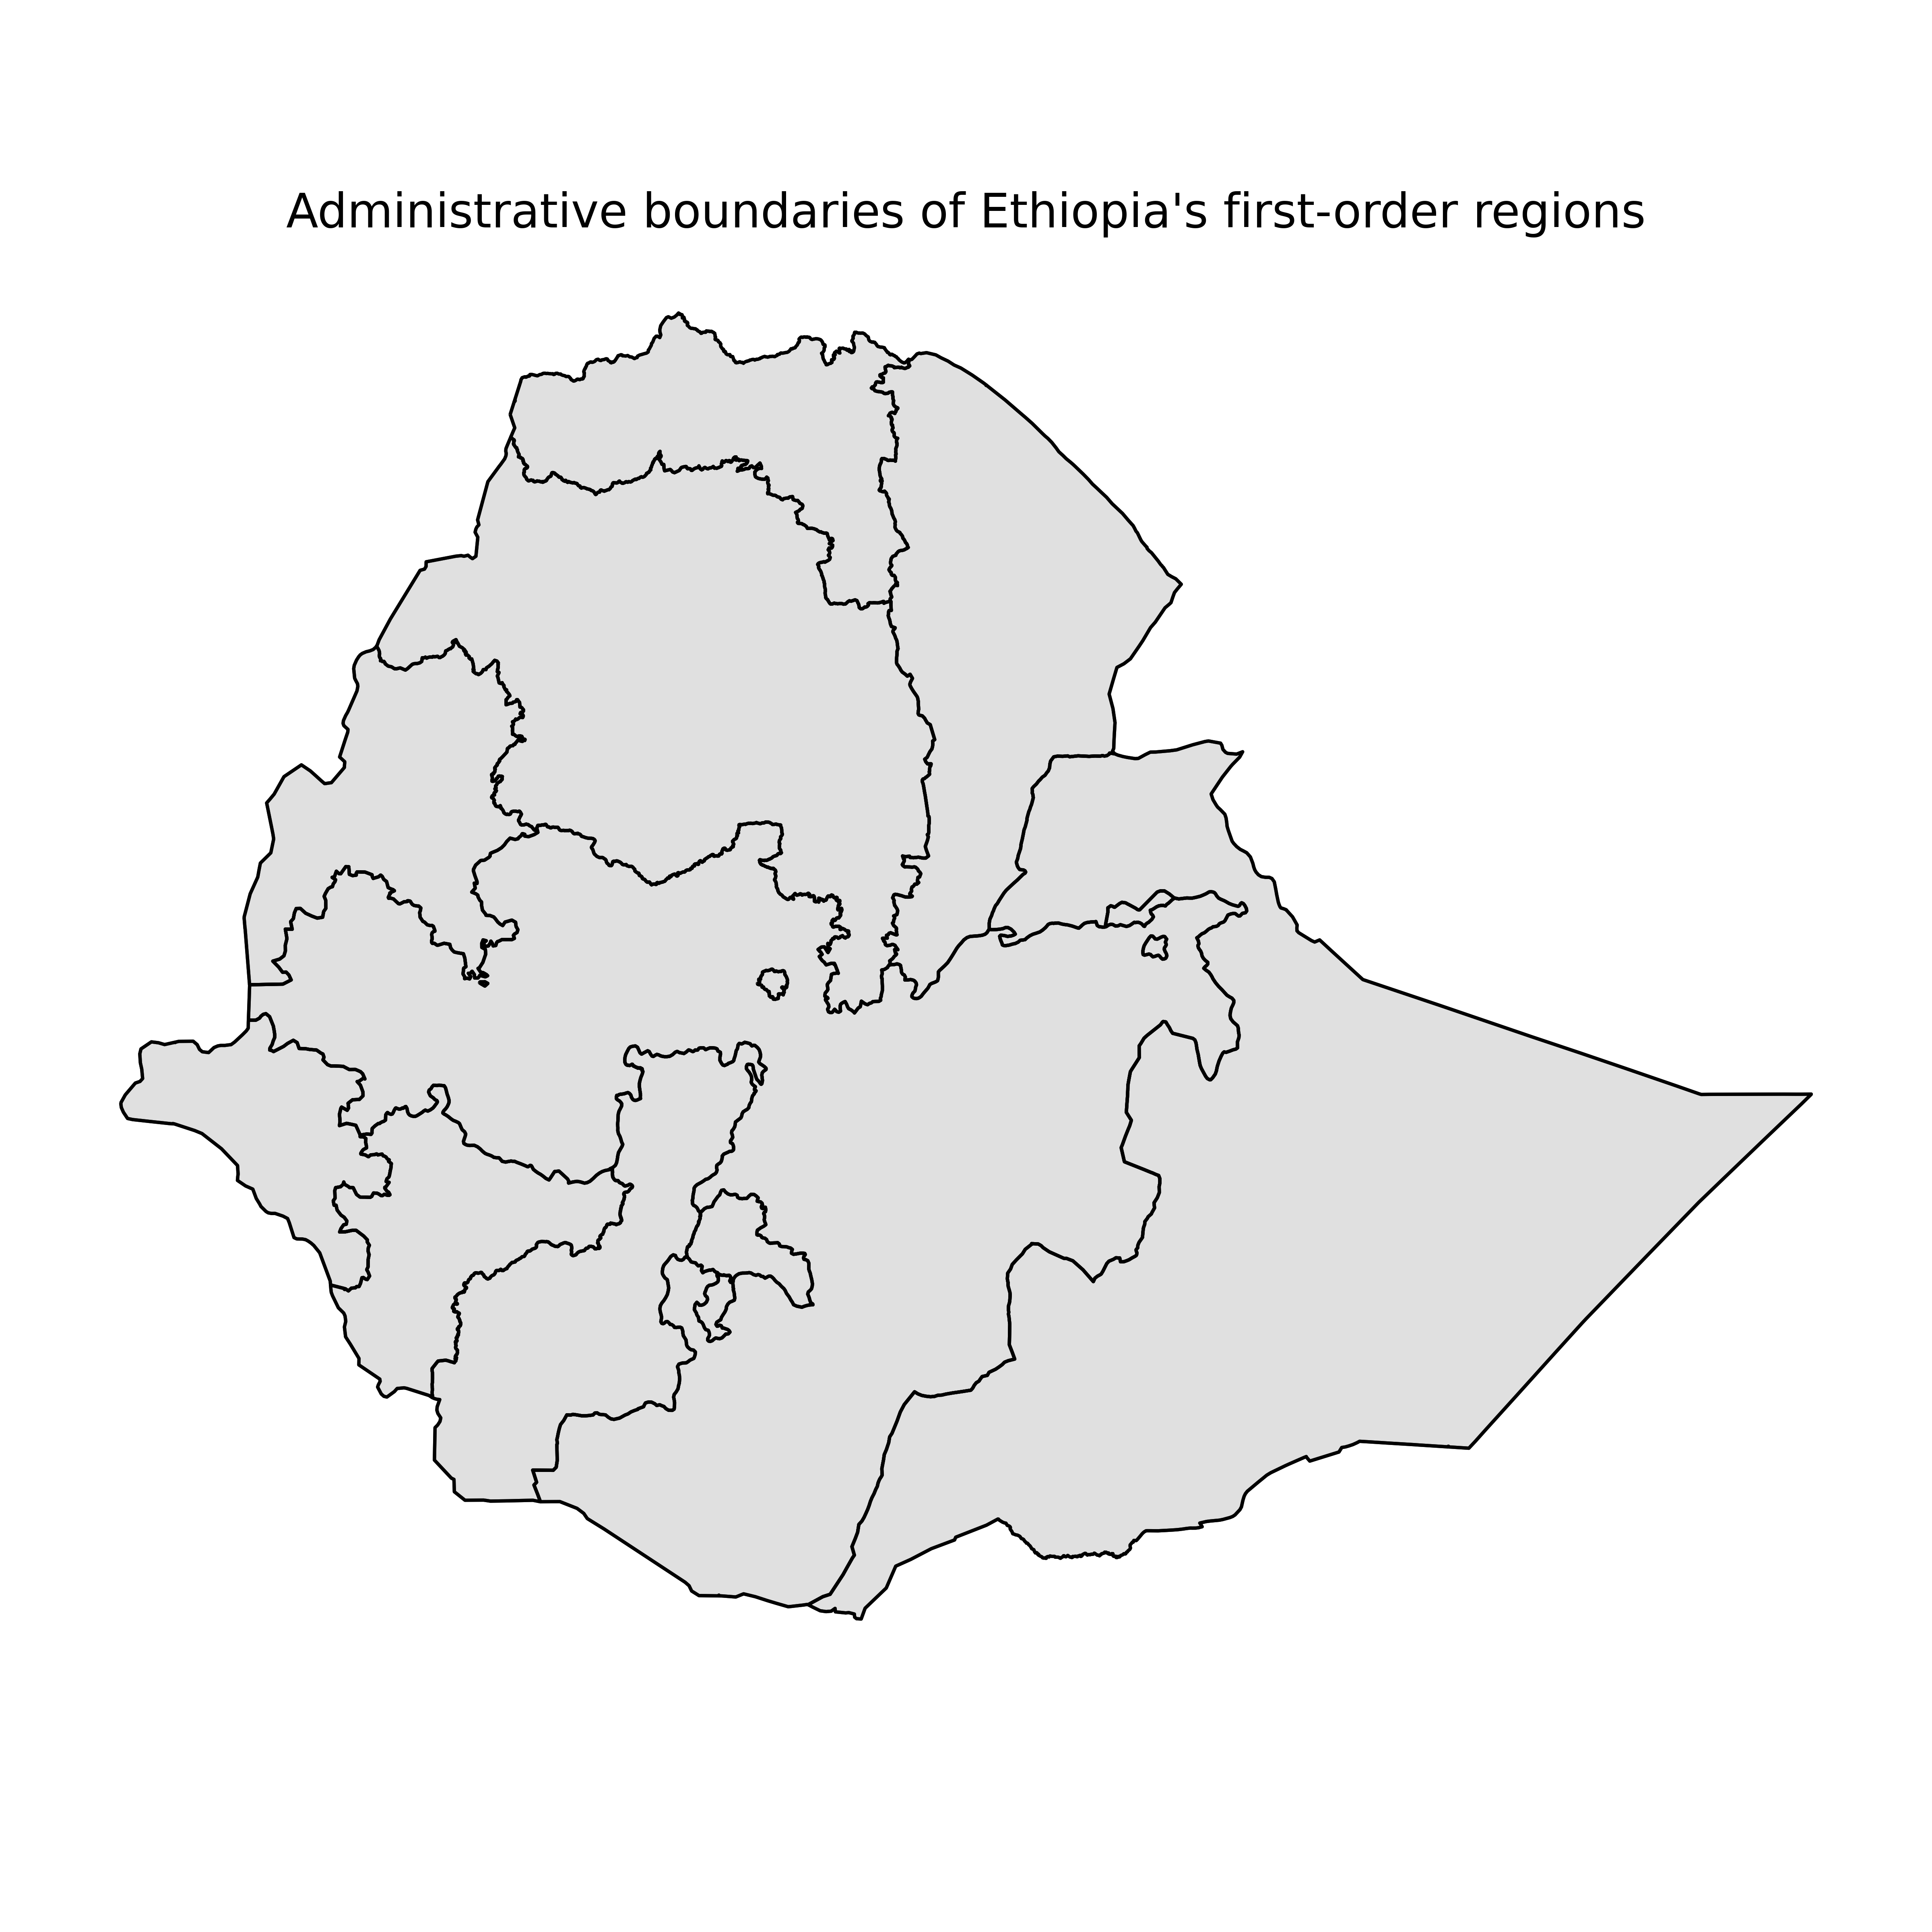
\includegraphics[width=0.7\textwidth]{outputs/figures/admin/ethiopia_admin_map.png}
	\caption{Administrative boundaries of Ethiopia's first-order regions. The map displays the 13 regional units used in the analysis, highlighting the evolving and fragmented nature of administrative boundaries over the study period.}
	\label{fig:admin_map}
\end{figure}
% --- End Figure 5 ---

\section{Identification Challenges in Small-N Panel Settings}

In empirical analyses of political favoritism using nighttime lights (NTL) data, identification is particularly challenging in settings with a small number of regions, limited exogenous variation in treatment, and high outcome concentration. This section outlines three core challenges that jointly limit inference in such panel data contexts.

\subsection{Omitted Variable Bias (without time fixed effects)}

When time fixed effects are omitted from panel regressions, estimates of leader-region favoritism are vulnerable to omitted variable bias. In the Ethiopian context, national economic shocks—such as booms or downturns—often coincide with leadership transitions. Without controlling for year effects, the estimated association between a leader’s birth region and regional luminosity may simply reflect these broader national trends, rather than any causal effect of political favoritism. Empirically, baseline models that exclude time fixed effects tend to produce inflated and statistically significant coefficients, but placebo tests and diagnostic plots reveal that these results are largely driven by common shocks rather than genuine treatment effects.

\subsection{Limited Identifying Variation (with time fixed effects)}

Including time fixed effects absorbs national shocks and common trends, but in small-N settings with few treated units and limited within-region, within-year variation, this approach introduces a new problem: limited identifying variation. When the timing of leader transitions is highly collinear with year effects, the model cannot reliably distinguish leader-region effects from national shocks. In the Ethiopian panel, the inclusion of time fixed effects sharply attenuates the estimated coefficients and increases standard errors, indicating that the available variation is insufficient for robust identification. The empirical p-values from placebo tests further confirm that observed effects are not distinguishable from random assignment.

\subsection{Low Statistical Power (small number of treated units)}

A third challenge is low statistical power, which arises from the small number of regions and limited number of leadership transitions. With only a handful of treated units and sparse treatment events, the effective sample size for identifying leader-region effects is severely constrained. This results in wide confidence intervals and imprecise estimates, particularly in event-study analyses and placebo simulations. The inability to detect dynamic effects or distinguish real from placebo results is a direct consequence of this low power, as demonstrated by the high empirical p-values and the overlap between observed and placebo distributions.

\paragraph{Synthesis}

Taken together, these challenges—omitted variable bias, limited identifying variation, and low statistical power—jointly undermine the credibility of causal inference in small-N panel settings. In the Ethiopian case, and in similar contexts, the combination of these factors means that apparent evidence for political favoritism is not empirically distinguishable from noise. Robust identification requires richer data, more exogenous variation, and careful diagnostic testing to avoid spurious findings.

\section{Literature Review}
This study sits at the intersection of three literatures.

First, a substantial literature uses satellite luminosity to measure economic activity. Early work established that light emissions track national and regional output surprisingly well in settings with limited conventional statistics \citep{Chen2011,Henderson2012}. More recent contributions show that the strength of this relationship varies with population density, sectoral composition, and spatial scale, which makes local interpretation more difficult than national validation exercises might suggest \citep{Bluhm2022,Gibson2021}. Work on harmonized long-run products has also improved the temporal comparability of DMSP-OLS and VIIRS series, but it has not eliminated measurement challenges \citep{Li2023,Gibson2024}.

Second, the paper relates to research on regional and ethnic favoritism. \citet{Hodler2014} show that political leaders' birth regions tend to receive higher nighttime light intensity in a broad cross-country sample. Subsequent work has refined that perspective by emphasizing the interaction between political favoritism, local ethnic demography, and institutions \citep{BeiserMcGrath2021}. Recent studies also continue to find geographically targeted favoritism in other settings, including public investment and local clientelism \citep{Onana2024,Cruzatti2024}. The implication is not that favoritism is universal, but that claims about it should be tested against within-unit changes rather than cross-sectional differences.




Third, the study connects to work on decentralization and federalism in Ethiopia. Existing scholarship highlights the tension between formal regional autonomy and persistent vertical control, including constraints on local fiscal autonomy and uneven developmental capacity \citep{Faguet2021,Wubneh2017}. Those institutional features make Ethiopia a theoretically important case for studying regional inequality, but they also heighten the need for careful empirical design. If regional trajectories differ for structural reasons unrelated to political leadership, pooled cross-sectional comparisons can easily be mistaken for favoritism.

\subsection*{Political Economy of Ethiopian Federalism}
The spatial distribution of rents in Ethiopia is deeply shaped by the country’s federal architecture and the political strategies of its ruling coalitions. Under the Ethiopian People’s Revolutionary Democratic Front (EPRDF), federalism was formally enshrined, but real power remained highly centralized. The EPRDF’s dominance over regional governments meant that resource allocation, investment, and development projects were often coordinated from the center, with regional administrations acting as agents rather than autonomous principals. This centralization is theorized to produce a spatial distribution of rents that is less responsive to local political dynamics and more reflective of national priorities and coalition management. In contrast, the current administration has presided over a period of greater regional contestation and, in some cases, increased regional autonomy. According to \citet{Faguet2021}, such shifts can alter the expected pattern of rent distribution: as regional governments gain more effective autonomy, the allocation of resources may become more sensitive to local political competition, ethnic demography, and the bargaining power of regional elites. This theoretical perspective suggests that the empirical analysis of favoritism in Ethiopia must account for changes in the structure of federalism and the evolving balance of power between center and regions.

Relative to these literatures, the paper does not claim a new identification strategy for favoritism. Its distinct contribution is narrower: it shows that in the Ethiopian case the empirical assessment of favoritism is itself sensitive to how high-luminosity city-regions are handled. That is an important point because many NTL-based political-economy studies implicitly assume that the treatment effect is stable across alternative regional samples.

\section{Methodology}
\subsection{Data}
\subsubsection{Nighttime light data}
The repository contains a harmonized annual NTL series built from DMSP-OLS and VIIRS raster products. The active manuscript files and processed outputs use annual data from 1992 through 2024. The underlying scripts reference the pixel-scale corrected nighttime light product of \citet{Li2023} and annual VIIRS composites derived by \citet{Elvidge2021}. Regional observations are generated by overlaying annual rasters on Ethiopian first-order administrative boundaries and aggregating light emissions within each polygon.

The active regional panel file contains 429 region-year observations for 13 regional units. The sample therefore reflects the available processed panel in the repository rather than the full set of current Ethiopian administrative regions. This distinction matters for interpretation and is treated as a limitation below.
% --- Begin Figure 5: Admin Map ---
\begin{figure}[ht]
	\centering
	% Replace the following line with the actual path to your admin map graphic
	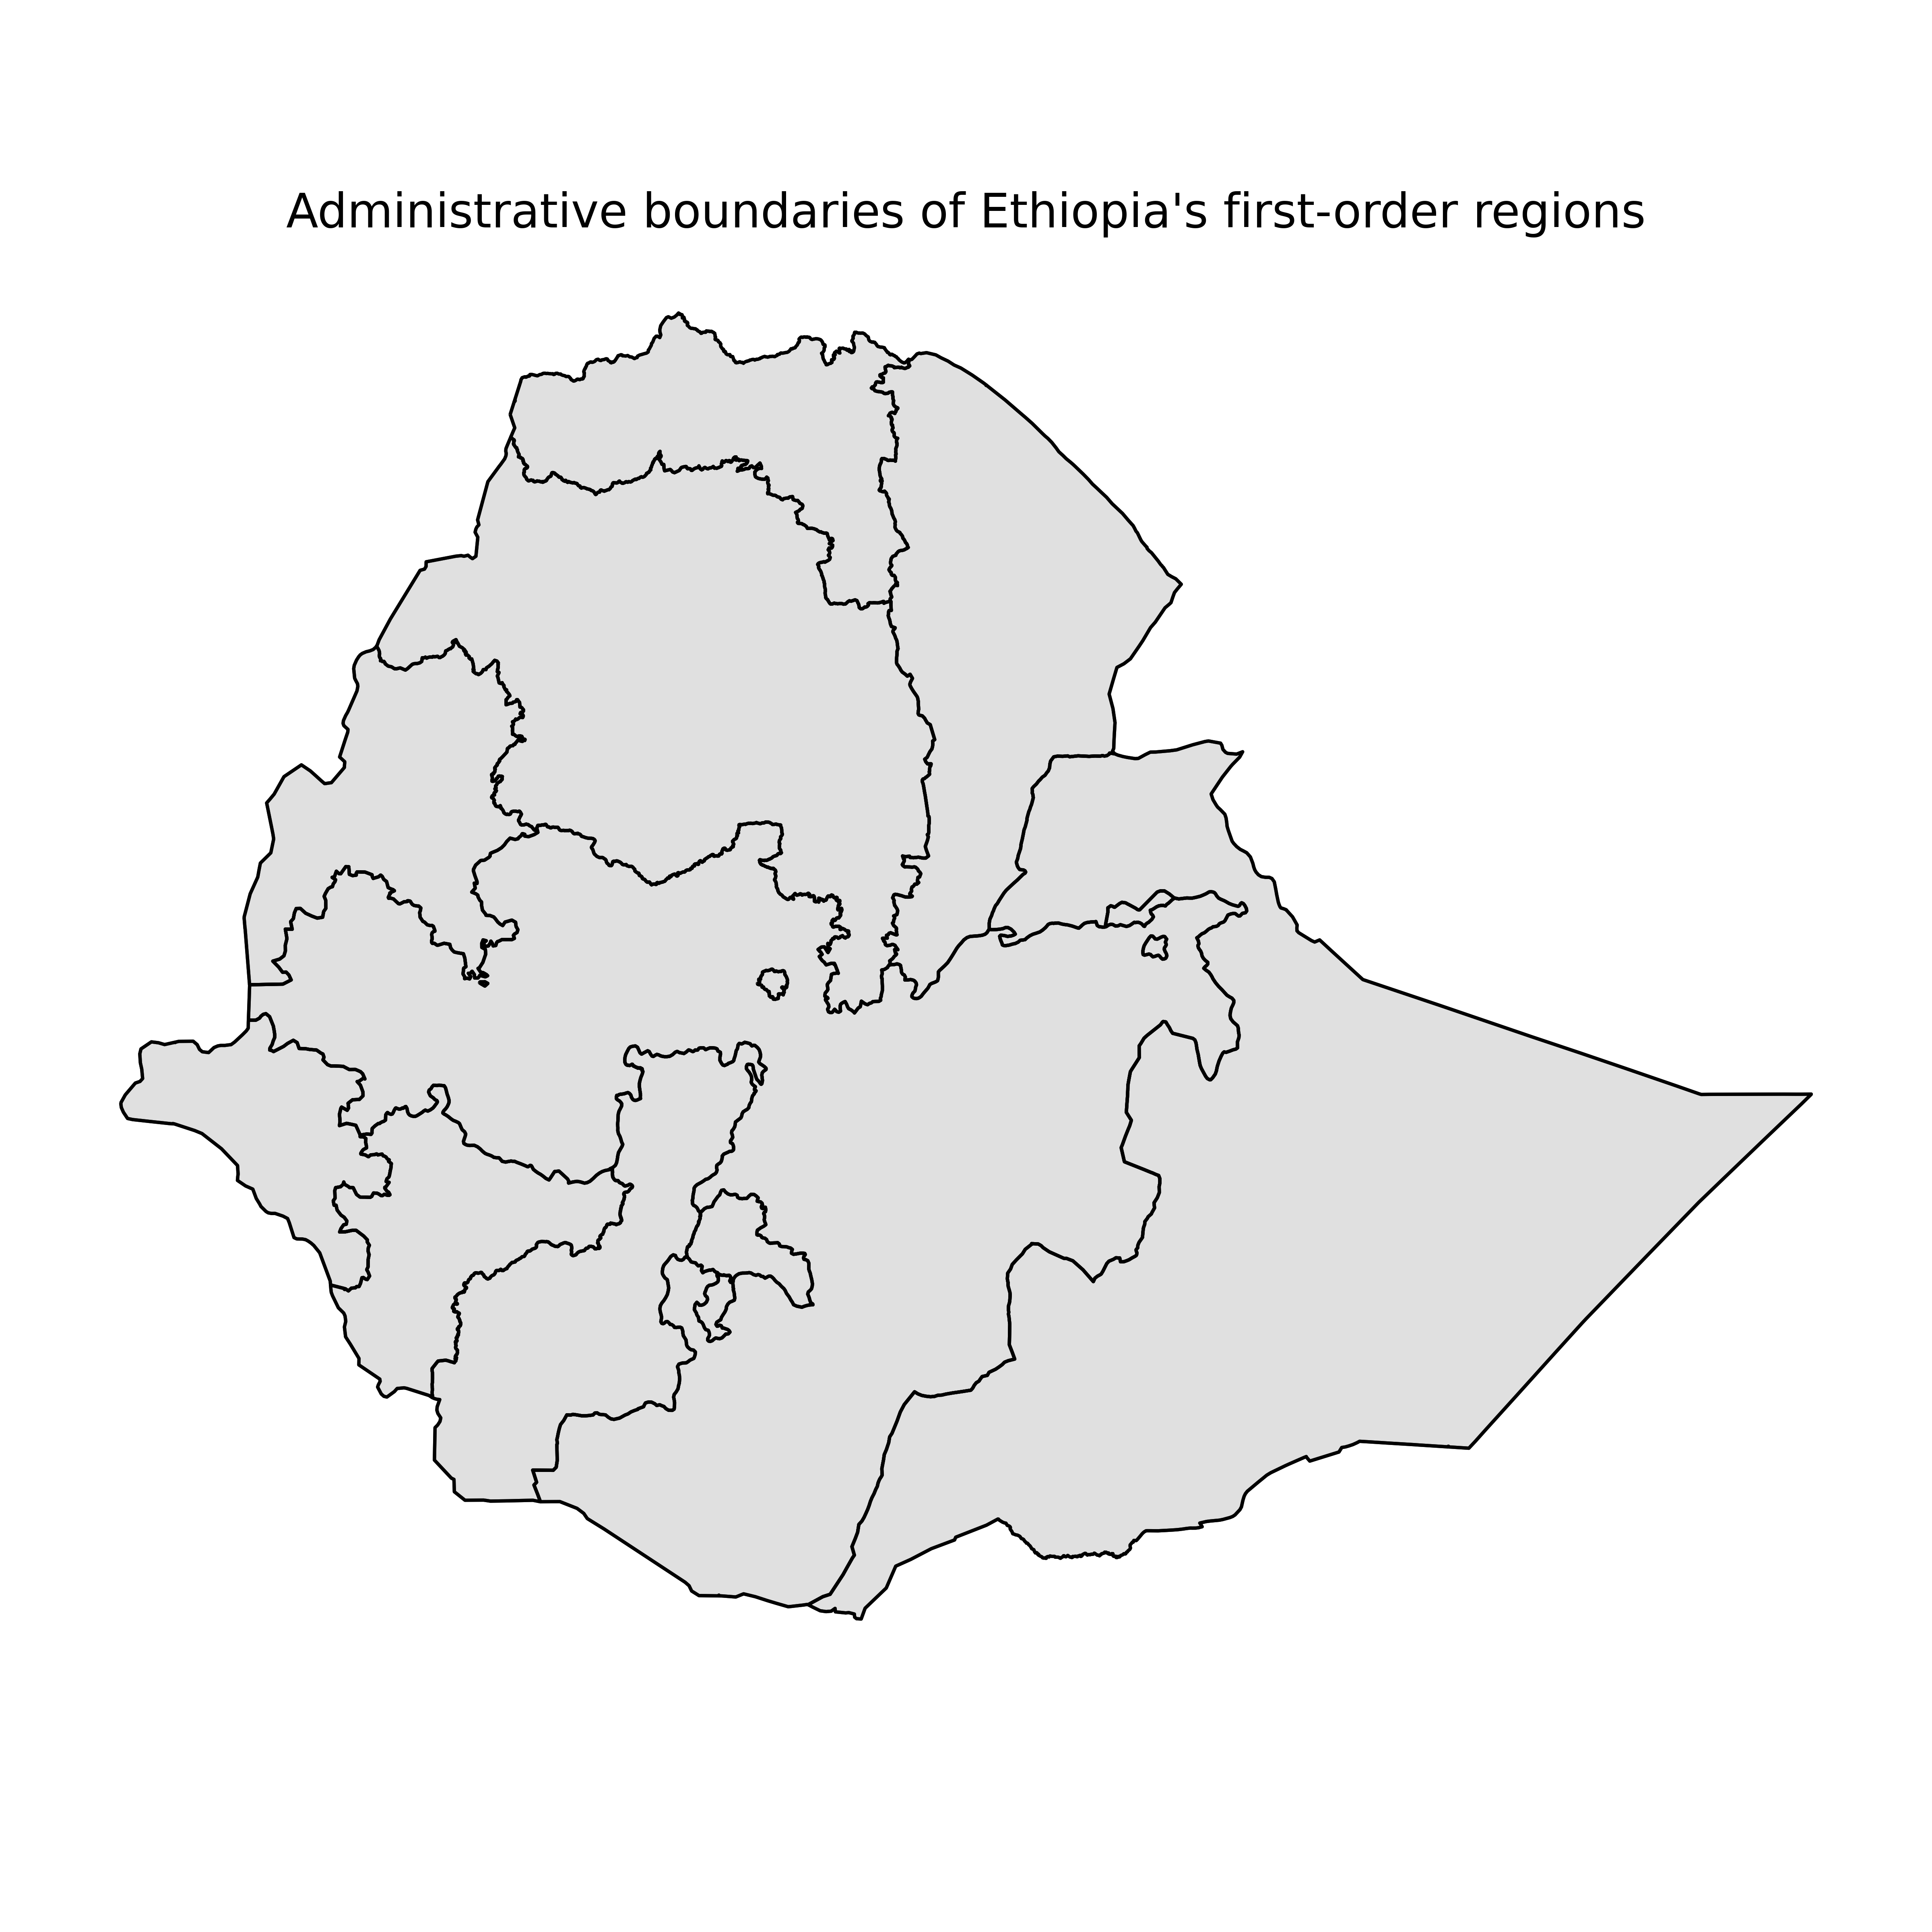
\includegraphics[width=0.7\textwidth]{outputs/figures/admin/ethiopia_admin_map.png}
	\caption{Administrative boundaries of Ethiopia's first-order regions. The map displays the 13 regional units used in the analysis, highlighting the evolving and fragmented nature of administrative boundaries over the study period.}
	\label{fig:admin_map}
\end{figure}
% --- End Figure 5 ---

\section{Identification Challenges in Small-N Panel Settings}

In empirical analyses of political favoritism using nighttime lights (NTL) data, identification is particularly challenging in settings with a small number of regions, limited exogenous variation in treatment, and high outcome concentration. This section outlines three core challenges that jointly limit inference in such panel data contexts.

\subsection{Omitted Variable Bias (without time fixed effects)}

When time fixed effects are omitted from panel regressions, estimates of leader-region favoritism are vulnerable to omitted variable bias. In the Ethiopian context, national economic shocks—such as booms or downturns—often coincide with leadership transitions. Without controlling for year effects, the estimated association between a leader’s birth region and regional luminosity may simply reflect these broader national trends, rather than any causal effect of political favoritism. Empirically, baseline models that exclude time fixed effects tend to produce inflated and statistically significant coefficients, but placebo tests and diagnostic plots reveal that these results are largely driven by common shocks rather than genuine treatment effects.

\subsection{Limited Identifying Variation (with time fixed effects)}

Including time fixed effects absorbs national shocks and common trends, but in small-N settings with few treated units and limited within-region, within-year variation, this approach introduces a new problem: limited identifying variation. When the timing of leader transitions is highly collinear with year effects, the model cannot reliably distinguish leader-region effects from national shocks. In the Ethiopian panel, the inclusion of time fixed effects sharply attenuates the estimated coefficients and increases standard errors, indicating that the available variation is insufficient for robust identification. The empirical p-values from placebo tests further confirm that observed effects are not distinguishable from random assignment.

\subsection{Low Statistical Power (small number of treated units)}

A third challenge is low statistical power, which arises from the small number of regions and limited number of leadership transitions. With only a handful of treated units and sparse treatment events, the effective sample size for identifying leader-region effects is severely constrained. This results in wide confidence intervals and imprecise estimates, particularly in event-study analyses and placebo simulations. The inability to detect dynamic effects or distinguish real from placebo results is a direct consequence of this low power, as demonstrated by the high empirical p-values and the overlap between observed and placebo distributions.

\paragraph{Synthesis}

Taken together, these challenges—omitted variable bias, limited identifying variation, and low statistical power—jointly undermine the credibility of causal inference in small-N panel settings. In the Ethiopian case, and in similar contexts, the combination of these factors means that apparent evidence for political favoritism is not empirically distinguishable from noise. Robust identification requires richer data, more exogenous variation, and careful diagnostic testing to avoid spurious findings.

\section{Literature Review}
This study sits at the intersection of three literatures.

First, a substantial literature uses satellite luminosity to measure economic activity. Early work established that light emissions track national and regional output surprisingly well in settings with limited conventional statistics \citep{Chen2011,Henderson2012}. More recent contributions show that the strength of this relationship varies with population density, sectoral composition, and spatial scale, which makes local interpretation more difficult than national validation exercises might suggest \citep{Bluhm2022,Gibson2021}. Work on harmonized long-run products has also improved the temporal comparability of DMSP-OLS and VIIRS series, but it has not eliminated measurement challenges \citep{Li2023,Gibson2024}.

Second, the paper relates to research on regional and ethnic favoritism. \citet{Hodler2014} show that political leaders' birth regions tend to receive higher nighttime light intensity in a broad cross-country sample. Subsequent work has refined that perspective by emphasizing the interaction between political favoritism, local ethnic demography, and institutions \citep{BeiserMcGrath2021}. Recent studies also continue to find geographically targeted favoritism in other settings, including public investment and local clientelism \citep{Onana2024,Cruzatti2024}. The implication is not that favoritism is universal, but that claims about it should be tested against within-unit changes rather than cross-sectional differences.




Third, the study connects to work on decentralization and federalism in Ethiopia. Existing scholarship highlights the tension between formal regional autonomy and persistent vertical control, including constraints on local fiscal autonomy and uneven developmental capacity \citep{Faguet2021,Wubneh2017}. Those institutional features make Ethiopia a theoretically important case for studying regional inequality, but they also heighten the need for careful empirical design. If regional trajectories differ for structural reasons unrelated to political leadership, pooled cross-sectional comparisons can easily be mistaken for favoritism.

\subsection*{Political Economy of Ethiopian Federalism}
The spatial distribution of rents in Ethiopia is deeply shaped by the country’s federal architecture and the political strategies of its ruling coalitions. Under the Ethiopian People’s Revolutionary Democratic Front (EPRDF), federalism was formally enshrined, but real power remained highly centralized. The EPRDF’s dominance over regional governments meant that resource allocation, investment, and development projects were often coordinated from the center, with regional administrations acting as agents rather than autonomous principals. This centralization is theorized to produce a spatial distribution of rents that is less responsive to local political dynamics and more reflective of national priorities and coalition management. In contrast, the current administration has presided over a period of greater regional contestation and, in some cases, increased regional autonomy. According to \citet{Faguet2021}, such shifts can alter the expected pattern of rent distribution: as regional governments gain more effective autonomy, the allocation of resources may become more sensitive to local political competition, ethnic demography, and the bargaining power of regional elites. This theoretical perspective suggests that the empirical analysis of favoritism in Ethiopia must account for changes in the structure of federalism and the evolving balance of power between center and regions.

Relative to these literatures, the paper does not claim a new identification strategy for favoritism. Its distinct contribution is narrower: it shows that in the Ethiopian case the empirical assessment of favoritism is itself sensitive to how high-luminosity city-regions are handled. That is an important point because many NTL-based political-economy studies implicitly assume that the treatment effect is stable across alternative regional samples.

\section{Methodology}
\subsection{Data}
\subsubsection{Nighttime light data}
The repository contains a harmonized annual NTL series built from DMSP-OLS and VIIRS raster products. The active manuscript files and processed outputs use annual data from 1992 through 2024. The underlying scripts reference the pixel-scale corrected nighttime light product of \citet{Li2023} and annual VIIRS composites derived by \citet{Elvidge2021}. Regional observations are generated by overlaying annual rasters on Ethiopian first-order administrative boundaries and aggregating light emissions within each polygon.

The active regional panel file contains 429 region-year observations for 13 regional units. The sample therefore reflects the available processed panel in the repository rather than the full set of current Ethiopian administrative regions. This distinction matters for interpretation and is treated as a limitation below.
% --- Begin Figure 5: Admin Map ---
\begin{figure}[ht]
	\centering
	% Replace the following line with the actual path to your admin map graphic
	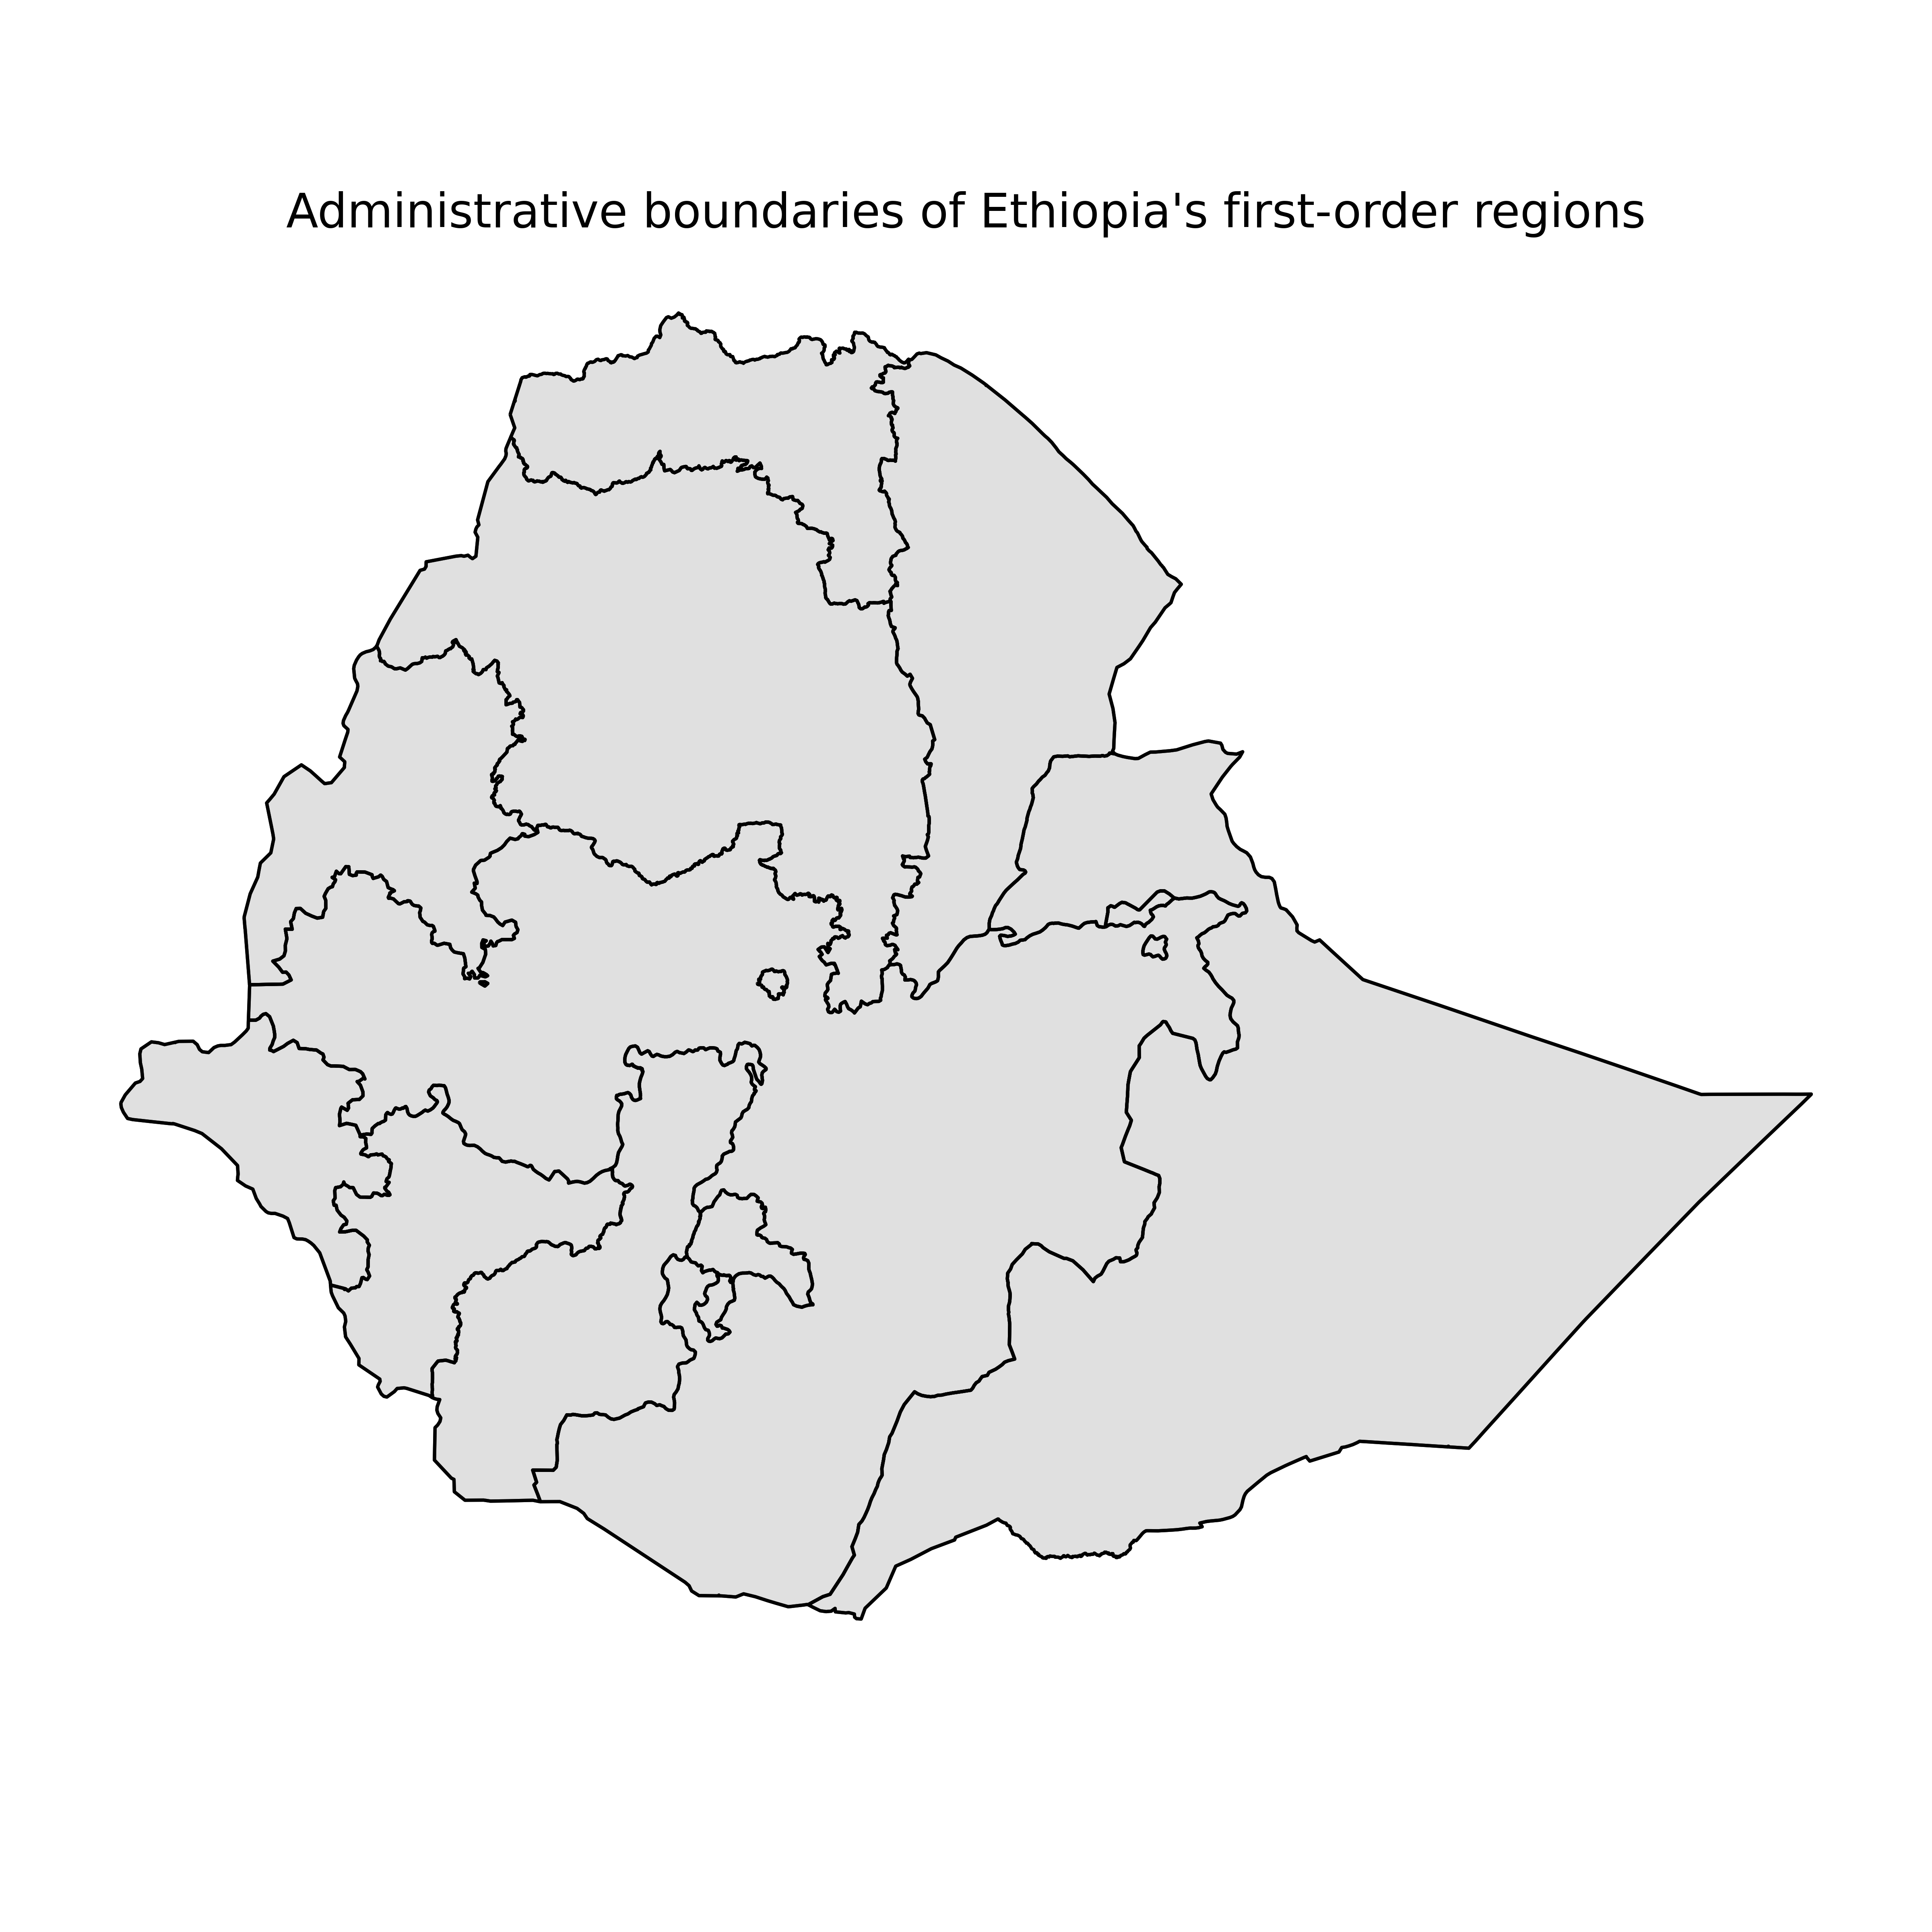
\includegraphics[width=0.7\textwidth]{outputs/figures/admin/ethiopia_admin_map.png}
	\caption{Administrative boundaries of Ethiopia's first-order regions. The map displays the 13 regional units used in the analysis, highlighting the evolving and fragmented nature of administrative boundaries over the study period.}
	\label{fig:admin_map}
\end{figure}
% --- End Figure 5 ---

\section{Identification Challenges in Small-N Panel Settings}

In empirical analyses of political favoritism using nighttime lights (NTL) data, identification is particularly challenging in settings with a small number of regions, limited exogenous variation in treatment, and high outcome concentration. This section outlines three core challenges that jointly limit inference in such panel data contexts.

\subsection{Omitted Variable Bias (without time fixed effects)}

When time fixed effects are omitted from panel regressions, estimates of leader-region favoritism are vulnerable to omitted variable bias. In the Ethiopian context, national economic shocks—such as booms or downturns—often coincide with leadership transitions. Without controlling for year effects, the estimated association between a leader’s birth region and regional luminosity may simply reflect these broader national trends, rather than any causal effect of political favoritism. Empirically, baseline models that exclude time fixed effects tend to produce inflated and statistically significant coefficients, but placebo tests and diagnostic plots reveal that these results are largely driven by common shocks rather than genuine treatment effects.

\subsection{Limited Identifying Variation (with time fixed effects)}

Including time fixed effects absorbs national shocks and common trends, but in small-N settings with few treated units and limited within-region, within-year variation, this approach introduces a new problem: limited identifying variation. When the timing of leader transitions is highly collinear with year effects, the model cannot reliably distinguish leader-region effects from national shocks. In the Ethiopian panel, the inclusion of time fixed effects sharply attenuates the estimated coefficients and increases standard errors, indicating that the available variation is insufficient for robust identification. The empirical p-values from placebo tests further confirm that observed effects are not distinguishable from random assignment.

\subsection{Low Statistical Power (small number of treated units)}

A third challenge is low statistical power, which arises from the small number of regions and limited number of leadership transitions. With only a handful of treated units and sparse treatment events, the effective sample size for identifying leader-region effects is severely constrained. This results in wide confidence intervals and imprecise estimates, particularly in event-study analyses and placebo simulations. The inability to detect dynamic effects or distinguish real from placebo results is a direct consequence of this low power, as demonstrated by the high empirical p-values and the overlap between observed and placebo distributions.

\paragraph{Synthesis}

Taken together, these challenges—omitted variable bias, limited identifying variation, and low statistical power—jointly undermine the credibility of causal inference in small-N panel settings. In the Ethiopian case, and in similar contexts, the combination of these factors means that apparent evidence for political favoritism is not empirically distinguishable from noise. Robust identification requires richer data, more exogenous variation, and careful diagnostic testing to avoid spurious findings.

\section{Literature Review}
This study sits at the intersection of three literatures.

First, a substantial literature uses satellite luminosity to measure economic activity. Early work established that light emissions track national and regional output surprisingly well in settings with limited conventional statistics \citep{Chen2011,Henderson2012}. More recent contributions show that the strength of this relationship varies with population density, sectoral composition, and spatial scale, which makes local interpretation more difficult than national validation exercises might suggest \citep{Bluhm2022,Gibson2021}. Work on harmonized long-run products has also improved the temporal comparability of DMSP-OLS and VIIRS series, but it has not eliminated measurement challenges \citep{Li2023,Gibson2024}.

Second, the paper relates to research on regional and ethnic favoritism. \citet{Hodler2014} show that political leaders' birth regions tend to receive higher nighttime light intensity in a broad cross-country sample. Subsequent work has refined that perspective by emphasizing the interaction between political favoritism, local ethnic demography, and institutions \citep{BeiserMcGrath2021}. Recent studies also continue to find geographically targeted favoritism in other settings, including public investment and local clientelism \citep{Onana2024,Cruzatti2024}. The implication is not that favoritism is universal, but that claims about it should be tested against within-unit changes rather than cross-sectional differences.




Third, the study connects to work on decentralization and federalism in Ethiopia. Existing scholarship highlights the tension between formal regional autonomy and persistent vertical control, including constraints on local fiscal autonomy and uneven developmental capacity \citep{Faguet2021,Wubneh2017}. Those institutional features make Ethiopia a theoretically important case for studying regional inequality, but they also heighten the need for careful empirical design. If regional trajectories differ for structural reasons unrelated to political leadership, pooled cross-sectional comparisons can easily be mistaken for favoritism.

\subsection*{Political Economy of Ethiopian Federalism}
The spatial distribution of rents in Ethiopia is deeply shaped by the country’s federal architecture and the political strategies of its ruling coalitions. Under the Ethiopian People’s Revolutionary Democratic Front (EPRDF), federalism was formally enshrined, but real power remained highly centralized. The EPRDF’s dominance over regional governments meant that resource allocation, investment, and development projects were often coordinated from the center, with regional administrations acting as agents rather than autonomous principals. This centralization is theorized to produce a spatial distribution of rents that is less responsive to local political dynamics and more reflective of national priorities and coalition management. In contrast, the current administration has presided over a period of greater regional contestation and, in some cases, increased regional autonomy. According to \citet{Faguet2021}, such shifts can alter the expected pattern of rent distribution: as regional governments gain more effective autonomy, the allocation of resources may become more sensitive to local political competition, ethnic demography, and the bargaining power of regional elites. This theoretical perspective suggests that the empirical analysis of favoritism in Ethiopia must account for changes in the structure of federalism and the evolving balance of power between center and regions.

Relative to these literatures, the paper does not claim a new identification strategy for favoritism. Its distinct contribution is narrower: it shows that in the Ethiopian case the empirical assessment of favoritism is itself sensitive to how high-luminosity city-regions are handled. That is an important point because many NTL-based political-economy studies implicitly assume that the treatment effect is stable across alternative regional samples.

\section{Methodology}
\subsection{Data}
\subsubsection{Nighttime light data}
The repository contains a harmonized annual NTL series built from DMSP-OLS and VIIRS raster products. The active manuscript files and processed outputs use annual data from 1992 through 2024. The underlying scripts reference the pixel-scale corrected nighttime light product of \citet{Li2023} and annual VIIRS composites derived by \citet{Elvidge2021}. Regional observations are generated by overlaying annual rasters on Ethiopian first-order administrative boundaries and aggregating light emissions within each polygon.

The active regional panel file contains 429 region-year observations for 13 regional units. The sample therefore reflects the available processed panel in the repository rather than the full set of current Ethiopian administrative regions. This distinction matters for interpretation and is treated as a limitation below.
% --- Begin Figure 5: Admin Map ---
\begin{figure}[ht]
	\centering
	% Replace the following line with the actual path to your admin map graphic
	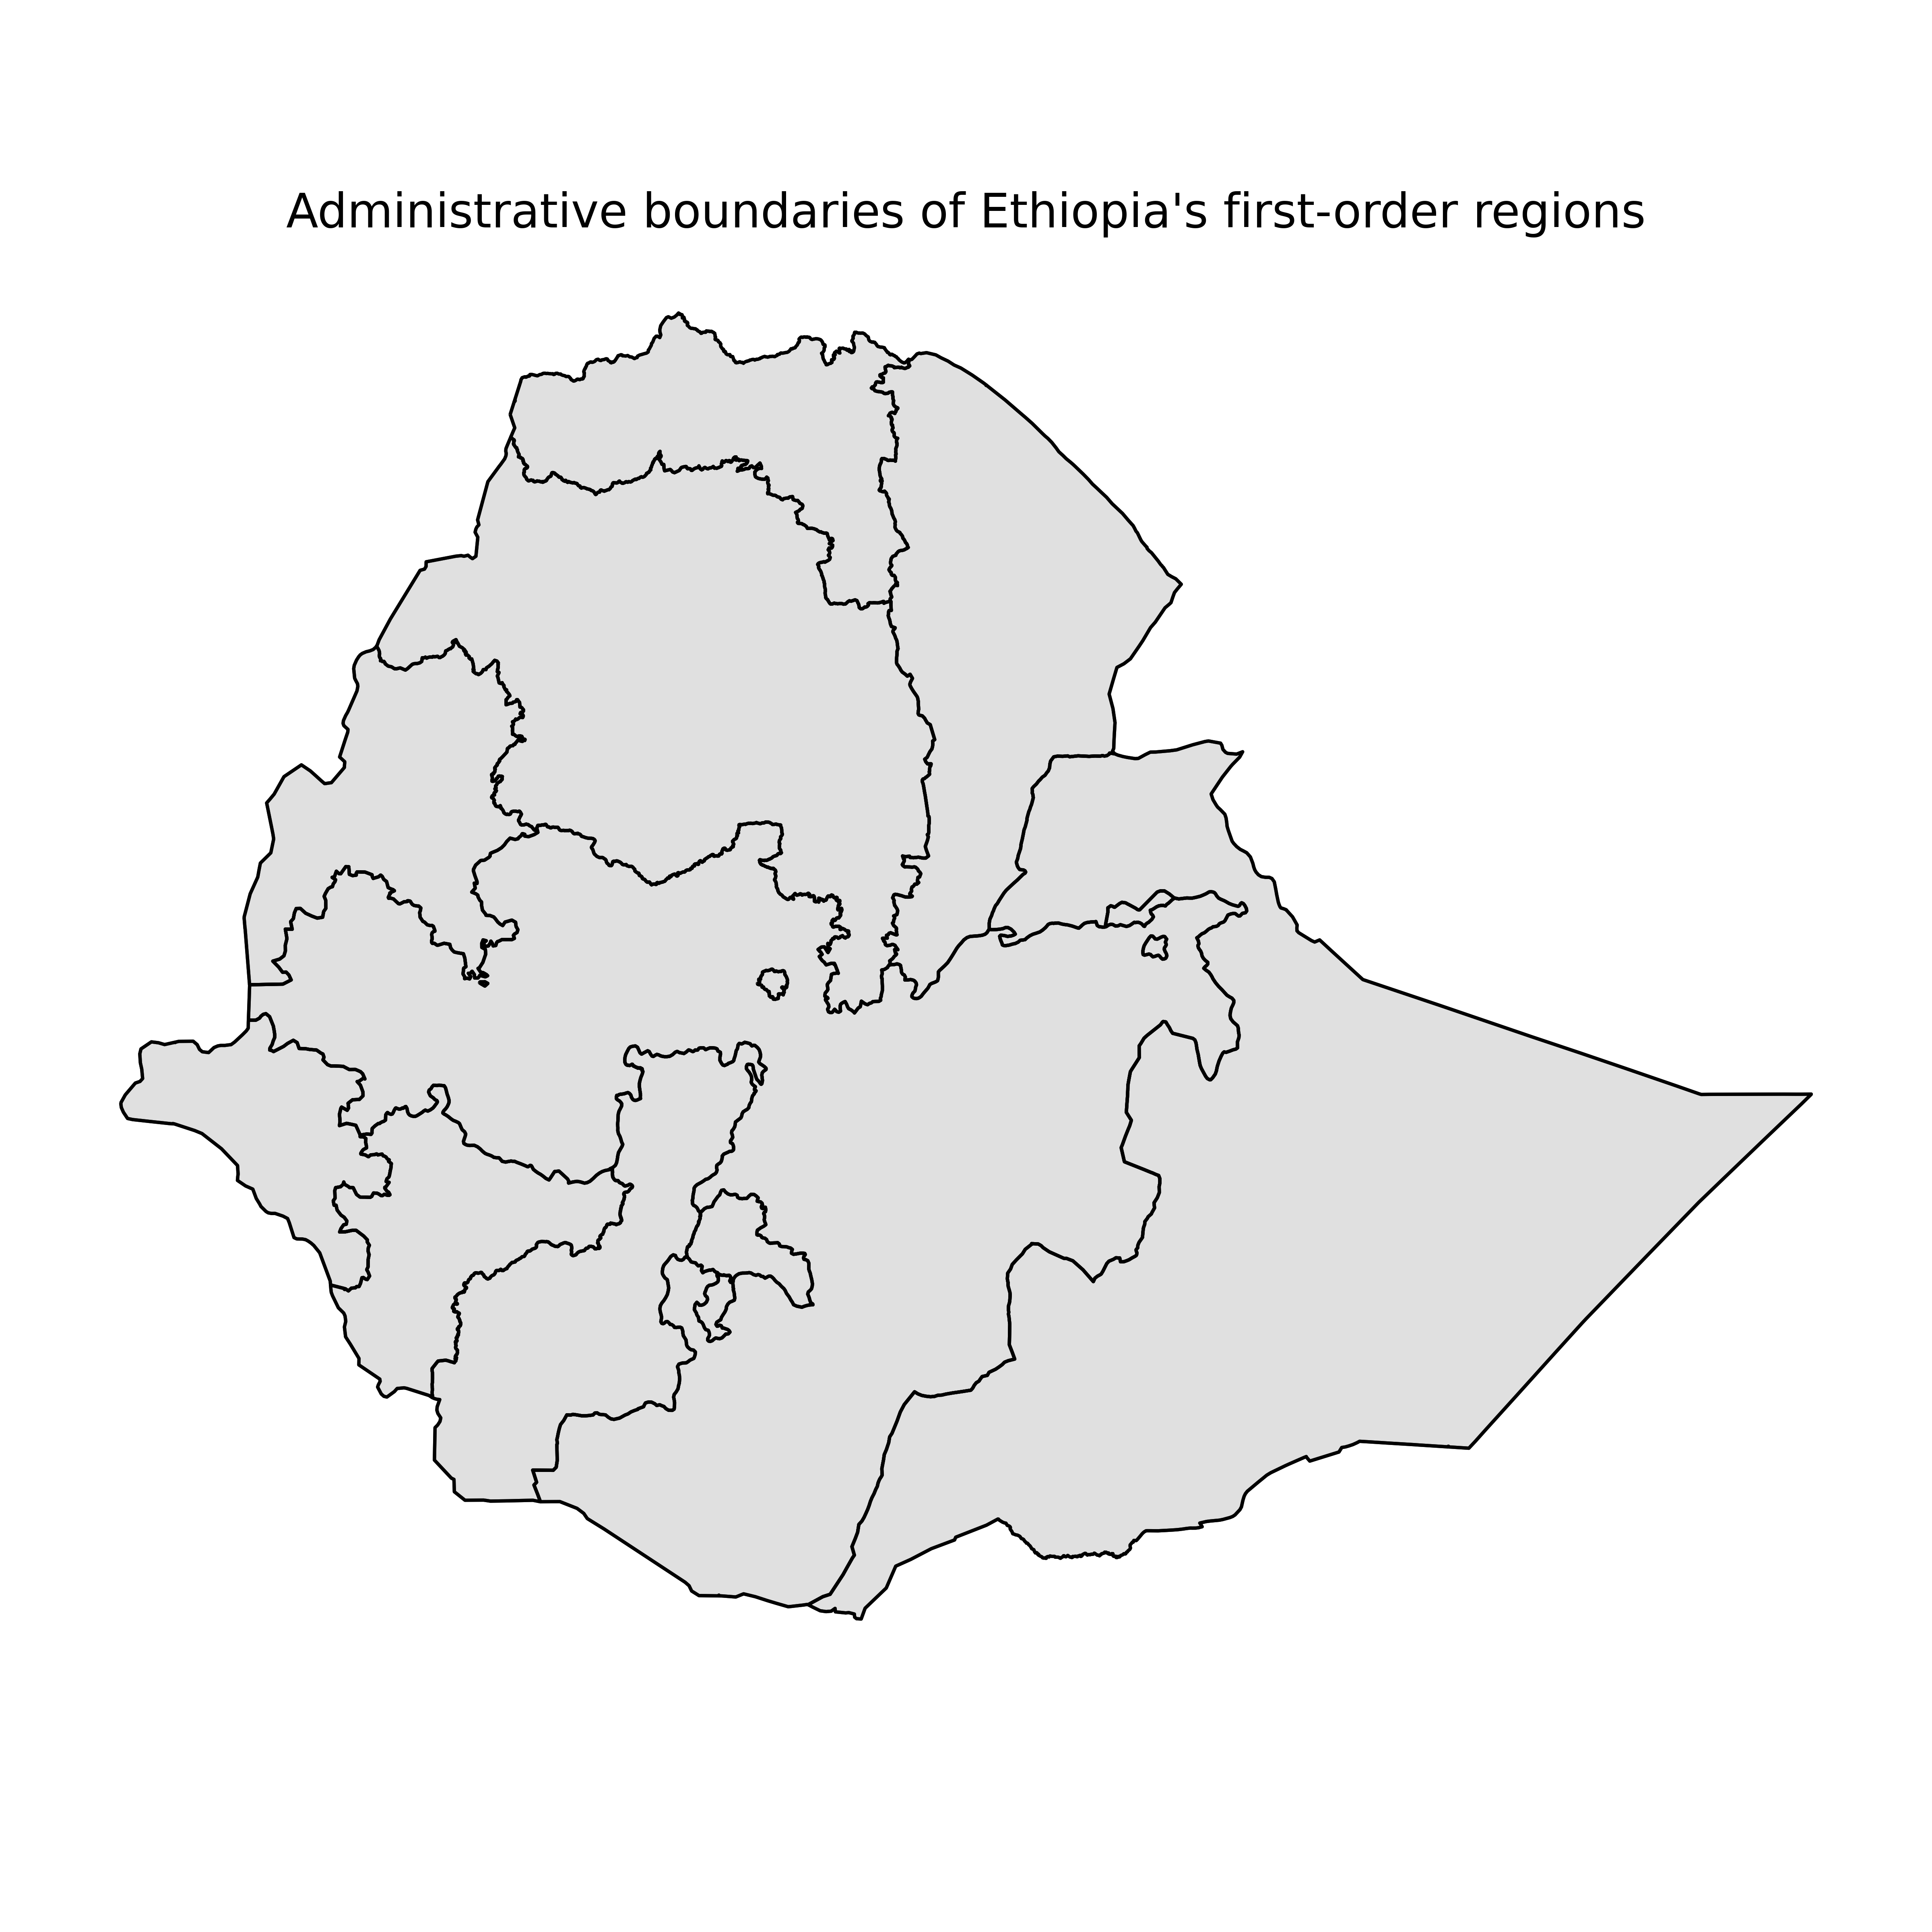
\includegraphics[width=0.7\textwidth]{outputs/figures/admin/ethiopia_admin_map.png}
	\caption{Administrative boundaries of Ethiopia's first-order regions. The map displays the 13 regional units used in the analysis, highlighting the evolving and fragmented nature of administrative boundaries over the study period.}
	\label{fig:admin_map}
\end{figure}
% --- End Figure 5 ---

\section{Identification Challenges in Small-N Panel Settings}

In empirical analyses of political favoritism using nighttime lights (NTL) data, identification is particularly challenging in settings with a small number of regions, limited exogenous variation in treatment, and high outcome concentration. This section outlines three core challenges that jointly limit inference in such panel data contexts.

\subsection{Omitted Variable Bias (without time fixed effects)}

When time fixed effects are omitted from panel regressions, estimates of leader-region favoritism are vulnerable to omitted variable bias. In the Ethiopian context, national economic shocks—such as booms or downturns—often coincide with leadership transitions. Without controlling for year effects, the estimated association between a leader’s birth region and regional luminosity may simply reflect these broader national trends, rather than any causal effect of political favoritism. Empirically, baseline models that exclude time fixed effects tend to produce inflated and statistically significant coefficients, but placebo tests and diagnostic plots reveal that these results are largely driven by common shocks rather than genuine treatment effects.

\subsection{Limited Identifying Variation (with time fixed effects)}

Including time fixed effects absorbs national shocks and common trends, but in small-N settings with few treated units and limited within-region, within-year variation, this approach introduces a new problem: limited identifying variation. When the timing of leader transitions is highly collinear with year effects, the model cannot reliably distinguish leader-region effects from national shocks. In the Ethiopian panel, the inclusion of time fixed effects sharply attenuates the estimated coefficients and increases standard errors, indicating that the available variation is insufficient for robust identification. The empirical p-values from placebo tests further confirm that observed effects are not distinguishable from random assignment.

\subsection{Low Statistical Power (small number of treated units)}

A third challenge is low statistical power, which arises from the small number of regions and limited number of leadership transitions. With only a handful of treated units and sparse treatment events, the effective sample size for identifying leader-region effects is severely constrained. This results in wide confidence intervals and imprecise estimates, particularly in event-study analyses and placebo simulations. The inability to detect dynamic effects or distinguish real from placebo results is a direct consequence of this low power, as demonstrated by the high empirical p-values and the overlap between observed and placebo distributions.

\paragraph{Synthesis}

Taken together, these challenges—omitted variable bias, limited identifying variation, and low statistical power—jointly undermine the credibility of causal inference in small-N panel settings. In the Ethiopian case, and in similar contexts, the combination of these factors means that apparent evidence for political favoritism is not empirically distinguishable from noise. Robust identification requires richer data, more exogenous variation, and careful diagnostic testing to avoid spurious findings.

\section{Literature Review}
This study sits at the intersection of three literatures.

First, a substantial literature uses satellite luminosity to measure economic activity. Early work established that light emissions track national and regional output surprisingly well in settings with limited conventional statistics \citep{Chen2011,Henderson2012}. More recent contributions show that the strength of this relationship varies with population density, sectoral composition, and spatial scale, which makes local interpretation more difficult than national validation exercises might suggest \citep{Bluhm2022,Gibson2021}. Work on harmonized long-run products has also improved the temporal comparability of DMSP-OLS and VIIRS series, but it has not eliminated measurement challenges \citep{Li2023,Gibson2024}.

Second, the paper relates to research on regional and ethnic favoritism. \citet{Hodler2014} show that political leaders' birth regions tend to receive higher nighttime light intensity in a broad cross-country sample. Subsequent work has refined that perspective by emphasizing the interaction between political favoritism, local ethnic demography, and institutions \citep{BeiserMcGrath2021}. Recent studies also continue to find geographically targeted favoritism in other settings, including public investment and local clientelism \citep{Onana2024,Cruzatti2024}. The implication is not that favoritism is universal, but that claims about it should be tested against within-unit changes rather than cross-sectional differences.




Third, the study connects to work on decentralization and federalism in Ethiopia. Existing scholarship highlights the tension between formal regional autonomy and persistent vertical control, including constraints on local fiscal autonomy and uneven developmental capacity \citep{Faguet2021,Wubneh2017}. Those institutional features make Ethiopia a theoretically important case for studying regional inequality, but they also heighten the need for careful empirical design. If regional trajectories differ for structural reasons unrelated to political leadership, pooled cross-sectional comparisons can easily be mistaken for favoritism.

\subsection*{Political Economy of Ethiopian Federalism}
The spatial distribution of rents in Ethiopia is deeply shaped by the country’s federal architecture and the political strategies of its ruling coalitions. Under the Ethiopian People’s Revolutionary Democratic Front (EPRDF), federalism was formally enshrined, but real power remained highly centralized. The EPRDF’s dominance over regional governments meant that resource allocation, investment, and development projects were often coordinated from the center, with regional administrations acting as agents rather than autonomous principals. This centralization is theorized to produce a spatial distribution of rents that is less responsive to local political dynamics and more reflective of national priorities and coalition management. In contrast, the current administration has presided over a period of greater regional contestation and, in some cases, increased regional autonomy. According to \citet{Faguet2021}, such shifts can alter the expected pattern of rent distribution: as regional governments gain more effective autonomy, the allocation of resources may become more sensitive to local political competition, ethnic demography, and the bargaining power of regional elites. This theoretical perspective suggests that

Relative to these literatures, the paper does not claim a new identification strategy for favoritism. Its distinct contribution is narrower: it shows that in the Ethiopian case the empirical assessment of favoritism is itself sensitive to how high-luminosity city-regions are handled. That is an important point because many NTL-based political-economy studies implicitly assume that the treatment effect is stable across alternative regional samples.

\section{Methodology}
\subsection{Data}
\subsubsection{Nighttime light data}
The repository contains a harmonized annual NTL series built from DMSP-OLS and VIIRS raster products. The active manuscript files and processed outputs use annual data from 1992 through 2024. The underlying scripts reference the pixel-scale corrected nighttime light product of \citet{Li2023} and annual VIIRS composites derived by \citet{Elvidge2021}. Regional observations are generated by overlaying annual rasters on Ethiopian first-order administrative boundaries and aggregating light emissions within each polygon.

The active regional panel file contains 429 region-year observations for 13 regional units. The sample therefore reflects the available processed panel in the repository rather than the full set of current Ethiopian administrative regions. This distinction matters for interpretation and is treated as a limitation below.
% --- Begin Figure 5: Admin Map ---
\begin{figure}[ht]
	\centering
	% Replace the following line with the actual path to your admin map graphic
	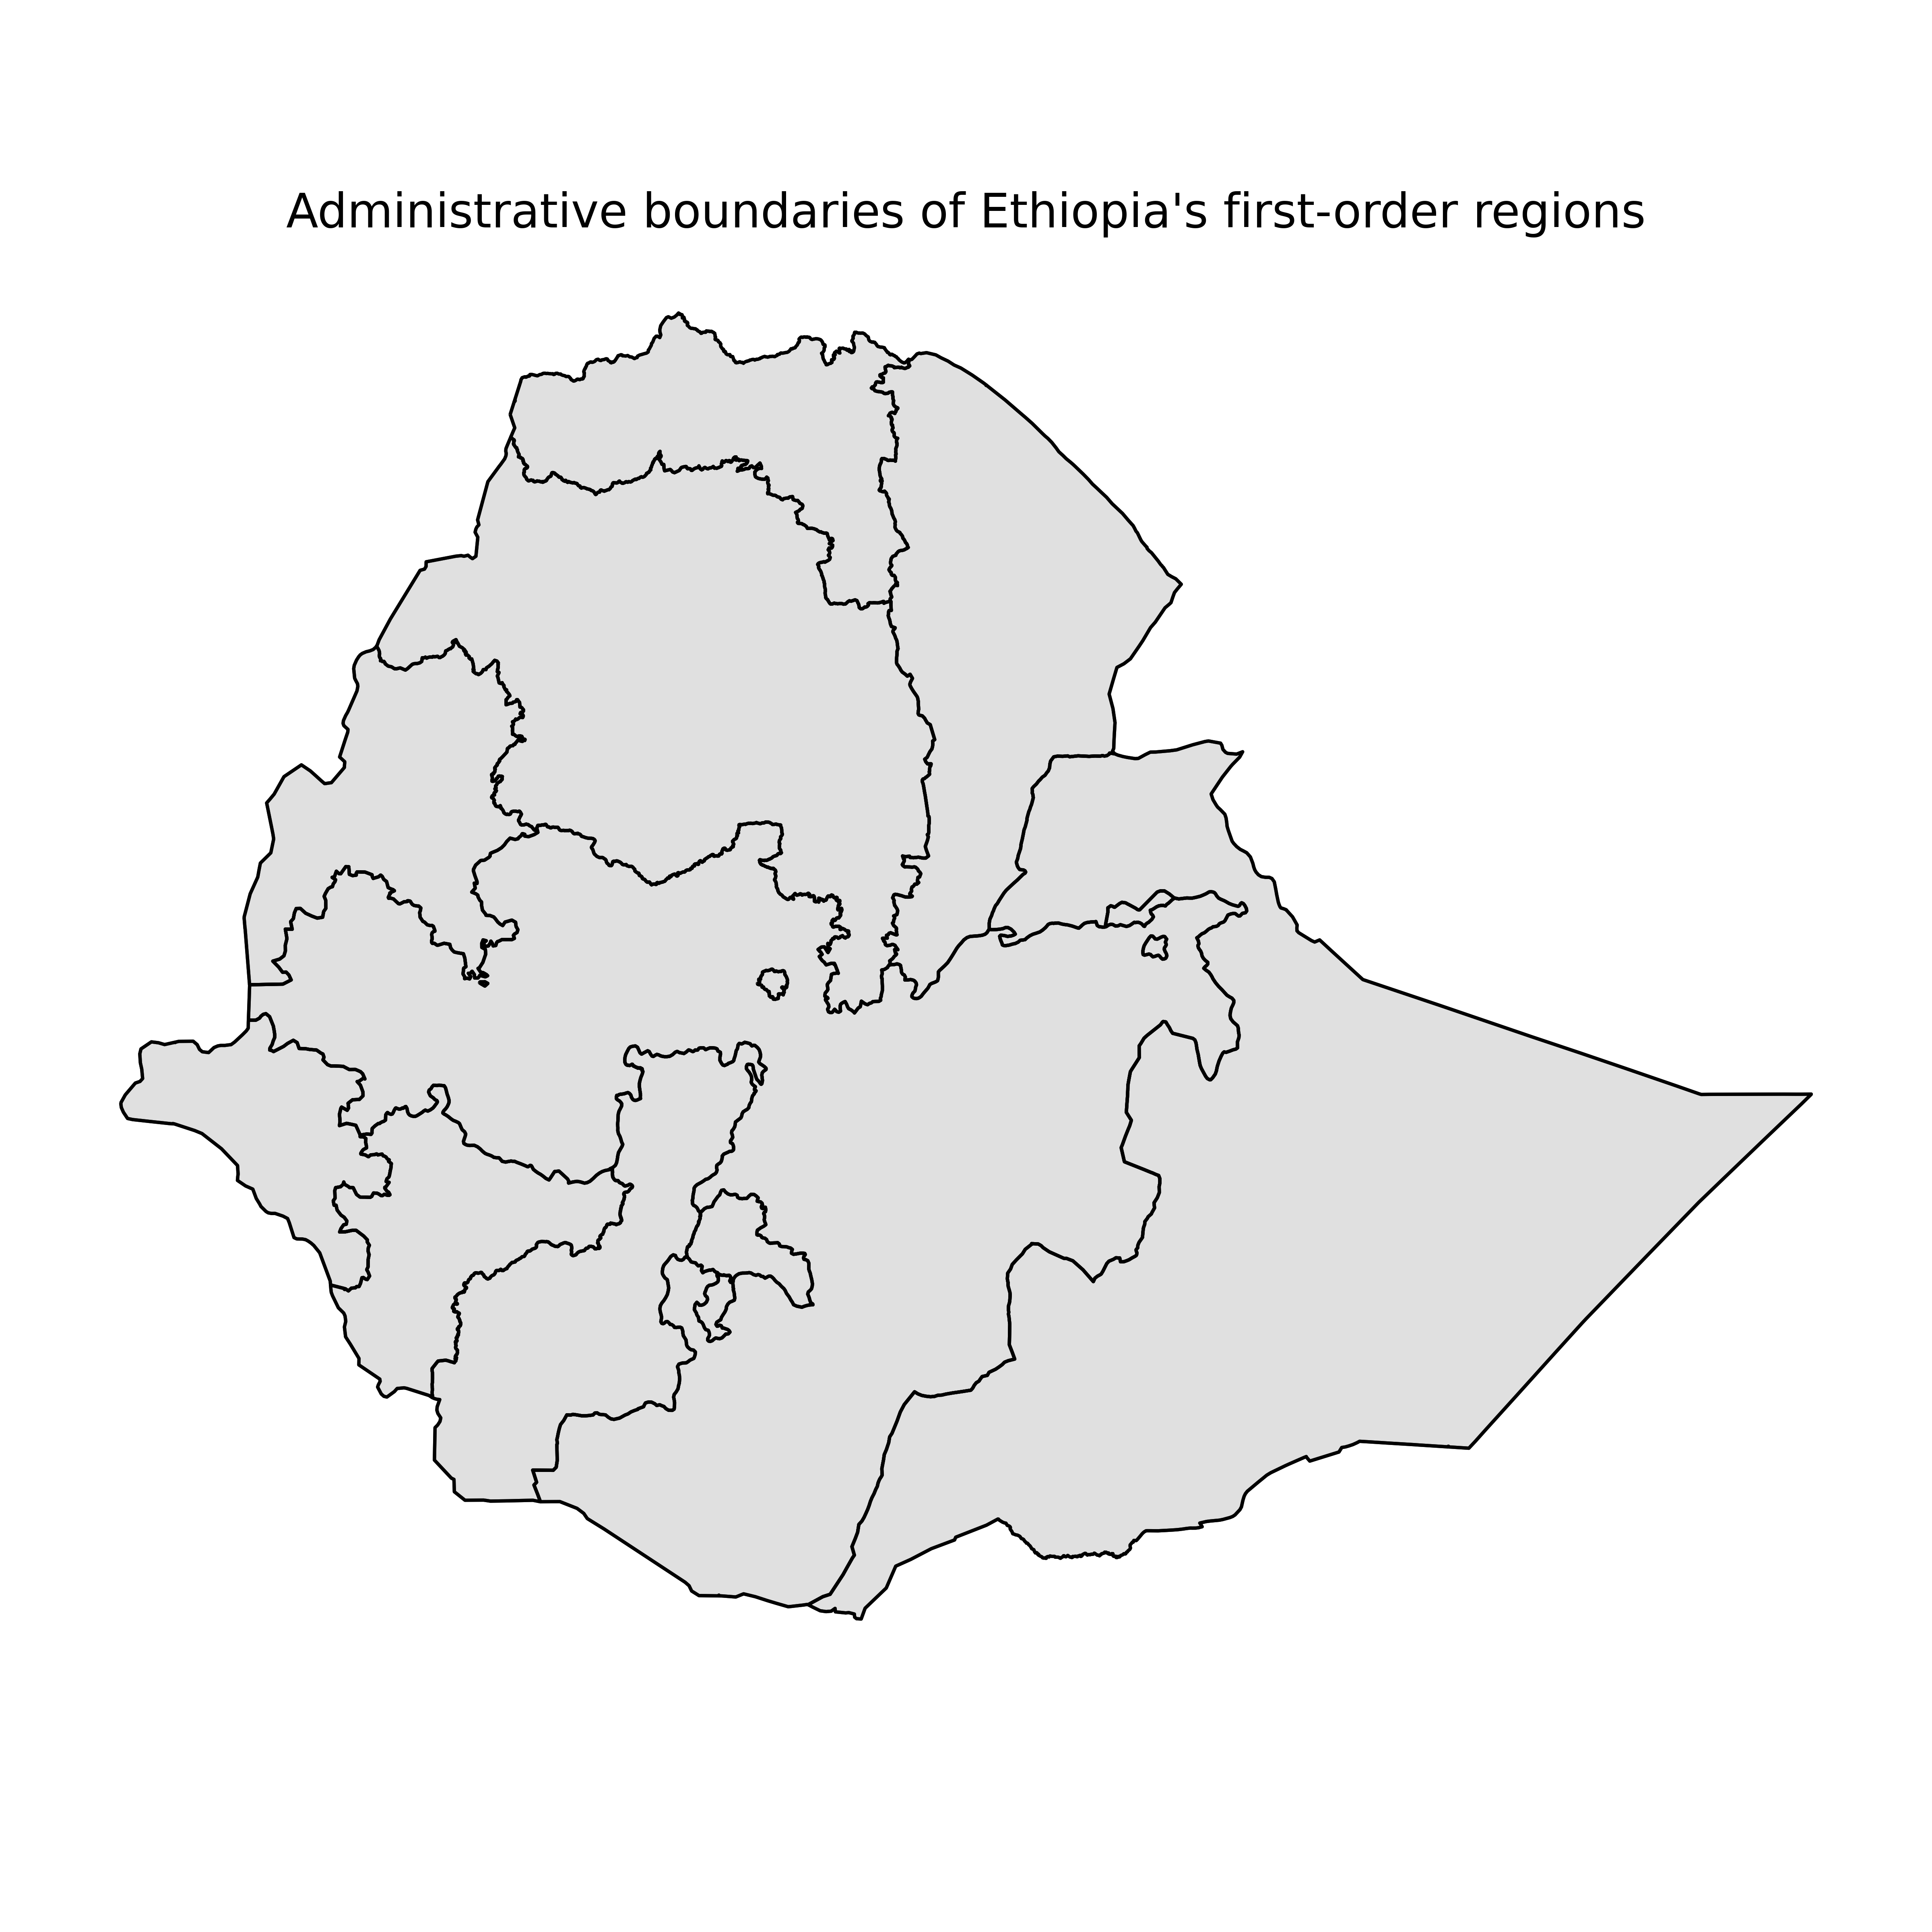
\includegraphics[width=0.7\textwidth]{outputs/figures/admin/ethiopia_admin_map.png}
	\caption{Administrative boundaries of Ethiopia's first-order regions. The map displays the 13 regional units used in the analysis, highlighting the evolving and fragmented nature of administrative boundaries over the study period.}
	\label{fig:admin_map}
\end{figure}
% --- End Figure 5 ---

\section{Identification Challenges in Small-N Panel Settings}

In empirical analyses of political favoritism using nighttime lights (NTL) data, identification is particularly challenging in settings with a small number of regions, limited exogenous variation in treatment, and high outcome concentration. This section outlines three core challenges that jointly limit inference in such panel data contexts.

\subsection{Omitted Variable Bias (without time fixed effects)}

When time fixed effects are omitted from panel regressions, estimates of leader-region favoritism are vulnerable to omitted variable bias. In the Ethiopian context, national economic shocks—such as booms or downturns—often coincide with leadership transitions. Without controlling for year effects, the estimated association between a leader’s birth region and regional luminosity may simply reflect these broader national trends, rather than any causal effect of political favoritism. Empirically, baseline models that exclude time fixed effects tend to produce inflated and statistically significant coefficients, but placebo tests and diagnostic plots reveal that these results are largely driven by common shocks rather than genuine treatment effects.

\subsection{Limited Identifying Variation (with time fixed effects)}

Including time fixed effects absorbs national shocks and common trends, but in small-N settings with few treated units and limited within-region, within-year variation, this approach introduces a new problem: limited identifying variation. When the timing of leader transitions is highly collinear with year effects, the model cannot reliably distinguish leader-region effects from national shocks. In the Ethiopian panel, the inclusion of time fixed effects sharply attenuates the estimated coefficients and increases standard errors, indicating that the available variation is insufficient for robust identification. The empirical p-values from placebo tests further confirm that observed effects are not distinguishable from random assignment.

\subsection{Low Statistical Power (small number of treated units)}

A third challenge is low statistical power, which arises from the small number of regions and limited number of leadership transitions. With only a handful of treated units and sparse treatment events, the effective sample size for identifying leader-region effects is severely constrained. This results in wide confidence intervals and imprecise estimates, particularly in event-study analyses and placebo simulations. The inability to detect dynamic effects or distinguish real from placebo results is a direct consequence of this low power, as demonstrated by the high empirical p-values and the overlap between observed and placebo distributions.

\paragraph{Synthesis}

Taken together, these challenges—omitted variable bias, limited identifying variation, and low statistical power—jointly undermine the credibility of causal inference in small-N panel settings. In the Ethiopian case, and in similar contexts, the combination of these factors means that apparent evidence for political favoritism is not empirically distinguishable from noise. Robust identification requires richer data, more exogenous variation, and careful diagnostic testing to avoid spurious findings.

\section{Literature Review}
This study sits at the intersection of three literatures.

First, a substantial literature uses satellite luminosity to measure economic activity. Early work established that light emissions track national and regional output surprisingly well in settings with limited conventional statistics \citep{Chen2011,Henderson2012}. More recent contributions show that the strength of this relationship varies with population density, sectoral composition, and spatial scale, which makes local interpretation more difficult than national validation exercises might suggest \citep{Bluhm2022,Gibson2021}. Work on harmonized long-run products has also improved the temporal comparability of DMSP-OLS and VIIRS series, but it has not eliminated measurement challenges \citep{Li2023,Gibson2024}.

Second, the paper relates to research on regional and ethnic favoritism. \citet{Hodler2014} show that political leaders' birth regions tend to receive higher nighttime light intensity in a broad cross-country sample. Subsequent work has refined that perspective by emphasizing the interaction between political favoritism, local ethnic demography, and institutions \citep{BeiserMcGrath2021}. Recent studies also continue to find geographically targeted favoritism in other settings, including public investment and local clientelism \citep{Onana2024,Cruzatti2024}. The implication is not that favoritism is universal, but that claims about it should be tested against within-unit changes rather than cross-sectional differences.




Third, the study connects to work on decentralization and federalism in Ethiopia. Existing scholarship highlights the tension between formal regional autonomy and persistent vertical control, including constraints on local fiscal autonomy and uneven developmental capacity \citep{Faguet2021,Wubneh2017}. Those institutional features make Ethiopia a theoretically important case for studying regional inequality, but they also heighten the need for careful empirical design. If regional trajectories differ for structural reasons unrelated to political leadership, pooled cross-sectional comparisons can easily be mistaken for favoritism.

\subsection*{Political Economy of Ethiopian Federalism}
The spatial distribution of rents in Ethiopia is deeply shaped by the country’s federal architecture and the political strategies of its ruling coalitions. Under the Ethiopian People’s Revolutionary Democratic Front (EPRDF), federalism was formally enshrined, but real power remained highly centralized. The EPRDF’s dominance over regional governments meant that resource allocation, investment, and development projects were often coordinated from the center, with regional administrations acting as agents rather than autonomous principals. This centralization is theorized to produce a spatial distribution of rents that is less responsive to local political dynamics and more reflective of national priorities and coalition management. In contrast, the current administration has presided over a period of greater regional contestation and, in some cases, increased regional autonomy. According to \citet{Faguet2021}, such shifts can alter the expected pattern of rent distribution: as regional governments gain more effective autonomy, the allocation of resources may become more sensitive to local political competition, ethnic demography, and the bargaining power of regional elites. This theoretical perspective suggests that the empirical analysis of favoritism in Ethiopia must account for changes in the structure of federalism and the evolving balance of power between center and regions.

Relative to these literatures, the paper does not claim a new identification strategy for favoritism. Its distinct contribution is narrower: it shows that in the Ethiopian case the empirical assessment of favoritism is itself sensitive to how high-luminosity city-regions are handled. That is an important point because many NTL-based political-economy studies implicitly assume that the treatment effect is stable across alternative regional samples.

\section{Methodology}
\subsection{Data}
\subsubsection{Nighttime light data}
The repository contains a harmonized annual NTL series built from DMSP-OLS and VIIRS raster products. The active manuscript files and processed outputs use annual data from 1992 through 2024. The underlying scripts reference the pixel-scale corrected nighttime light product of \citet{Li2023} and annual VIIRS composites derived by \citet{Elvidge2021}. Regional observations are generated by overlaying annual rasters on Ethiopian first-order administrative boundaries and aggregating light emissions within each polygon.

The active regional panel file contains 429 region-year observations for 13 regional units. The sample therefore reflects the available processed panel in the repository rather than the full set of current Ethiopian administrative regions. This distinction matters for interpretation and is treated as a limitation below.
% --- Begin Figure 5: Admin Map ---
\begin{figure}[ht]
	\centering
	% Replace the following line with the actual path to your admin map graphic
	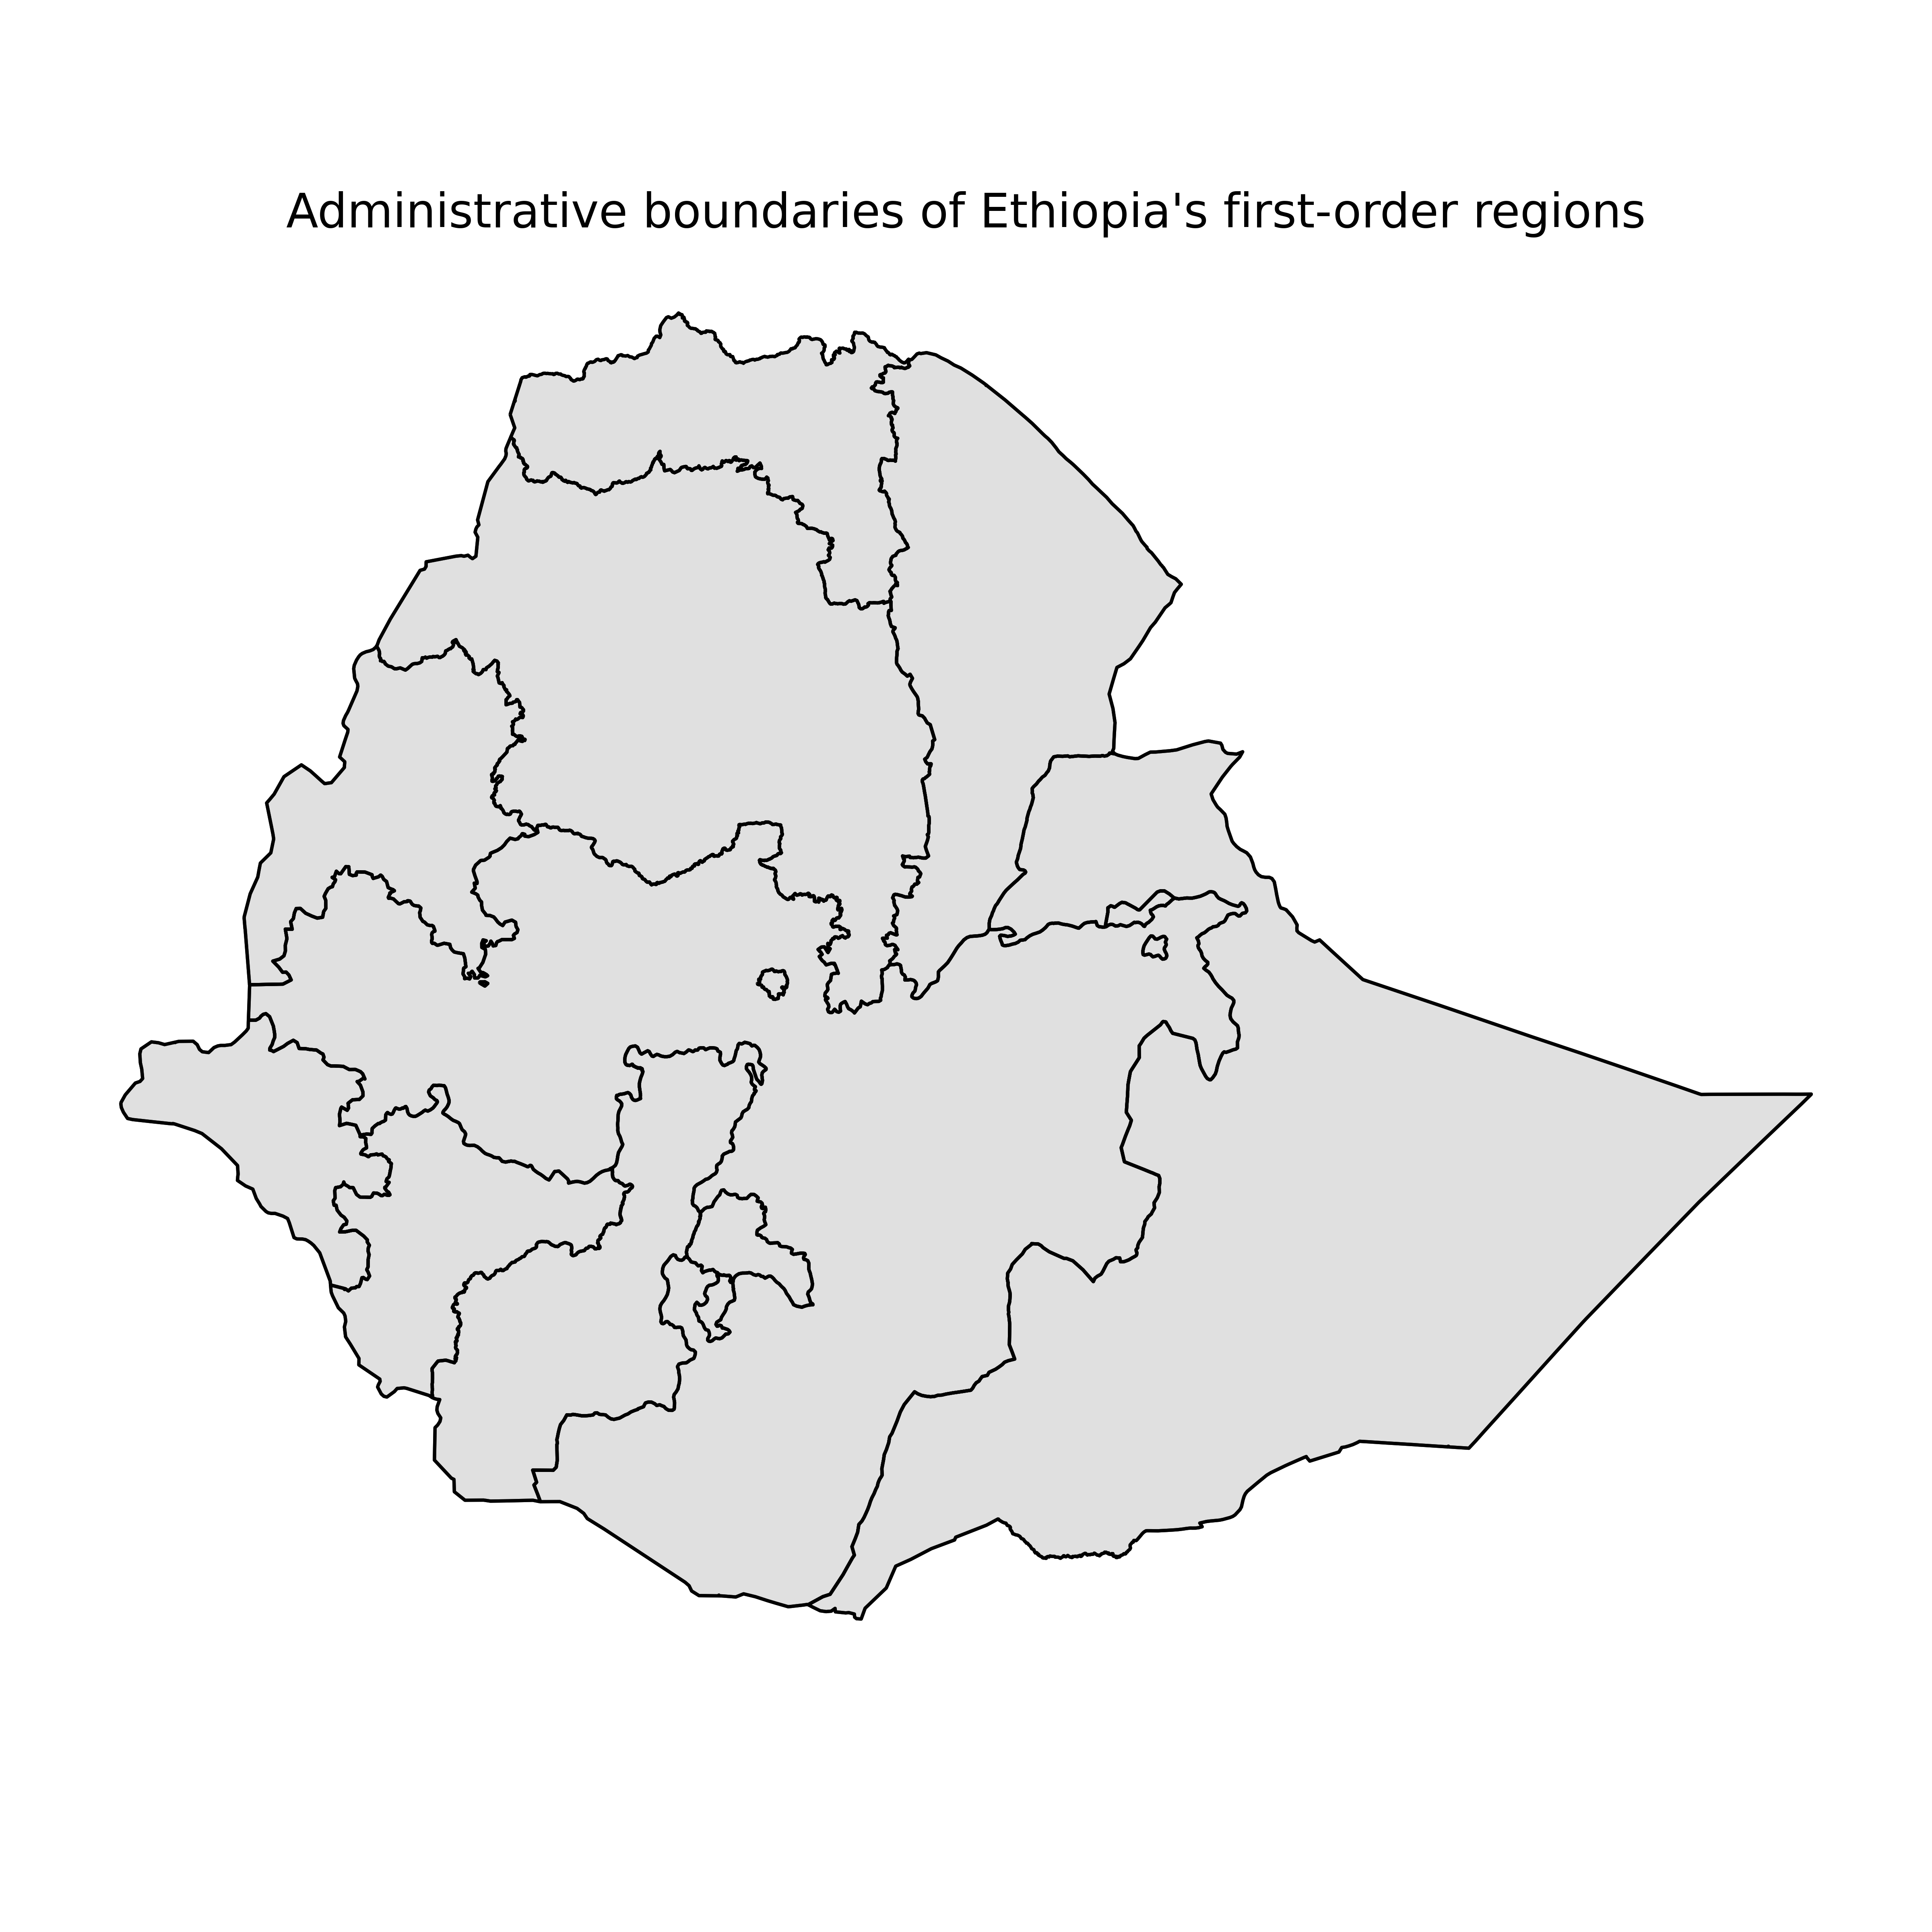
\includegraphics[width=0.7\textwidth]{outputs/figures/admin/ethiopia_admin_map.png}
	\caption{Administrative boundaries of Ethiopia's first-order regions. The map displays the 13 regional units used in the analysis, highlighting the evolving and fragmented nature of administrative boundaries over the study period.}
	\label{fig:admin_map}
\end{figure}
% --- End Figure 5 ---

\section{Identification Challenges in Small-N Panel Settings}

In empirical analyses of political favoritism using nighttime lights (NTL) data, identification is particularly challenging in settings with a small number of regions, limited exogenous variation in treatment, and high outcome concentration. This section outlines three core challenges that jointly limit inference in such panel data contexts.

\subsection{Omitted Variable Bias (without time fixed effects)}

When time fixed effects are omitted from panel regressions, estimates of leader-region favoritism are vulnerable to omitted variable bias. In the Ethiopian context, national economic shocks—such as booms or downturns—often coincide with leadership transitions. Without controlling for year effects, the estimated association between a leader’s birth region and regional luminosity may simply reflect these broader national trends, rather than any causal effect of political favoritism. Empirically, baseline models that exclude time fixed effects tend to produce inflated and statistically significant coefficients, but placebo tests and diagnostic plots reveal that these results are largely driven by common shocks rather than genuine treatment effects.

\subsection{Limited Identifying Variation (with time fixed effects)}

Including time fixed effects absorbs national shocks and common trends, but in small-N settings with few treated units and limited within-region, within-year variation, this approach introduces a new problem: limited identifying variation. When the timing of leader transitions is highly collinear with year effects, the model cannot reliably distinguish leader-region effects from national shocks. In the Ethiopian panel, the inclusion of time fixed effects sharply attenuates the estimated coefficients and increases standard errors, indicating that the available variation is insufficient for robust identification. The empirical p-values from placebo tests further confirm that observed effects are not distinguishable from random assignment.

\subsection{Low Statistical Power (small number of treated units)}

A third challenge is low statistical power, which arises from the small number of regions and limited number of leadership transitions. With only a handful of treated units and sparse treatment events, the effective sample size for identifying leader-region effects is severely constrained. This results in wide confidence intervals and imprecise estimates, particularly in event-study analyses and placebo simulations. The inability to detect dynamic effects or distinguish real from placebo results is a direct consequence of this low power, as demonstrated by the high empirical p-values and the overlap between observed and placebo distributions.

\paragraph{Synthesis}

Taken together, these challenges—omitted variable bias, limited identifying variation, and low statistical power—jointly undermine the credibility of causal inference in small-N panel settings. In the Ethiopian case, and in similar contexts, the combination of these factors means that apparent evidence for political favoritism is not empirically distinguishable from noise. Robust identification requires richer data, more exogenous variation, and careful diagnostic testing to avoid spurious findings.

\section{Literature Review}
This study sits at the intersection of three literatures.

First, a substantial literature uses satellite luminosity to measure economic activity. Early work established that light emissions track national and regional output surprisingly well in settings with limited conventional statistics \citep{Chen2011,Henderson2012}. More recent contributions show that the strength of this relationship varies with population density, sectoral composition, and spatial scale, which makes local interpretation more difficult than national validation exercises might suggest \citep{Bluhm2022,Gibson2021}. Work on harmonized long-run products has also improved the temporal comparability of DMSP-OLS and VIIRS series, but it has not eliminated measurement challenges \citep{Li2023,Gibson2024}.

Second, the paper relates to research on regional and ethnic favoritism. \citet{Hodler2014} show that political leaders' birth regions tend to receive higher nighttime light intensity in a broad cross-country sample. Subsequent work has refined that perspective by emphasizing the interaction between political favoritism, local ethnic demography, and institutions \citep{BeiserMcGrath2021}. Recent studies also continue to find geographically targeted favoritism in other settings, including public investment and local clientelism \citep{Onana2024,Cruzatti2024}. The implication is not that favoritism is universal, but that claims about it should be tested against within-unit changes rather than cross-sectional differences.




Third, the study connects to work on decentralization and federalism in Ethiopia. Existing scholarship highlights the tension between formal regional autonomy and persistent vertical control, including constraints on local fiscal autonomy and uneven developmental capacity \citep{Faguet2021,Wubneh2017}. Those institutional features make Ethiopia a theoretically important case for studying regional inequality, but they also heighten the need for careful empirical design. If regional trajectories differ for structural reasons unrelated to political leadership, pooled cross-sectional comparisons can easily be mistaken for favoritism.

\subsection*{Political Economy of Ethiopian Federalism}
The spatial distribution of rents in Ethiopia is deeply shaped by the country’s federal architecture and the political strategies of its ruling coalitions. Under the Ethiopian People’s Revolutionary Democratic Front (EPRDF), federalism was formally enshrined, but real power remained highly centralized. The EPRDF’s dominance over regional governments meant that resource allocation, investment, and development projects were often coordinated from the center, with regional administrations acting as agents rather than autonomous principals. This centralization is theorized to produce a spatial distribution of rents that is less responsive to local political dynamics and more reflective of national priorities and coalition management. In contrast, the current administration has presided over a period of greater regional contestation and, in some cases, increased regional autonomy. According to \citet{Faguet2021}, such shifts can alter the expected pattern of rent distribution: as regional governments gain more effective autonomy, the allocation of resources may become more sensitive to local political competition, ethnic demography, and the bargaining power of regional elites. This theoretical perspective suggests that the empirical analysis of favoritism in Ethiopia must account for changes in the structure of federalism and the evolving balance of power between center and regions.

Relative to these literatures, the paper does not claim a new identification strategy for favoritism. Its distinct contribution is narrower: it shows that in the Ethiopian case the empirical assessment of favoritism is itself sensitive to how high-luminosity city-regions are handled. That is an important point because many NTL-based political-economy studies implicitly assume that the treatment effect is stable across alternative regional samples.

\section{Methodology}
\subsection{Data}
\subsubsection{Nighttime light data}
The repository contains a harmonized annual NTL series built from DMSP-OLS and VIIRS raster products. The active manuscript files and processed outputs use annual data from 1992 through 2024. The underlying scripts reference the pixel-scale corrected nighttime light product of \citet{Li2023} and annual VIIRS composites derived by \citet{Elvidge2021}. Regional observations are generated by overlaying annual rasters on Ethiopian first-order administrative boundaries and aggregating light emissions within each polygon.

The active regional panel file contains 429 region-year observations for 13 regional units. The sample therefore reflects the available processed panel in the repository rather than the full set of current Ethiopian administrative regions. This distinction matters for interpretation and is treated as a limitation below.
% --- Begin Figure 5: Admin Map ---
\begin{figure}[ht]
	\centering
	% Replace the following line with the actual path to your admin map graphic
	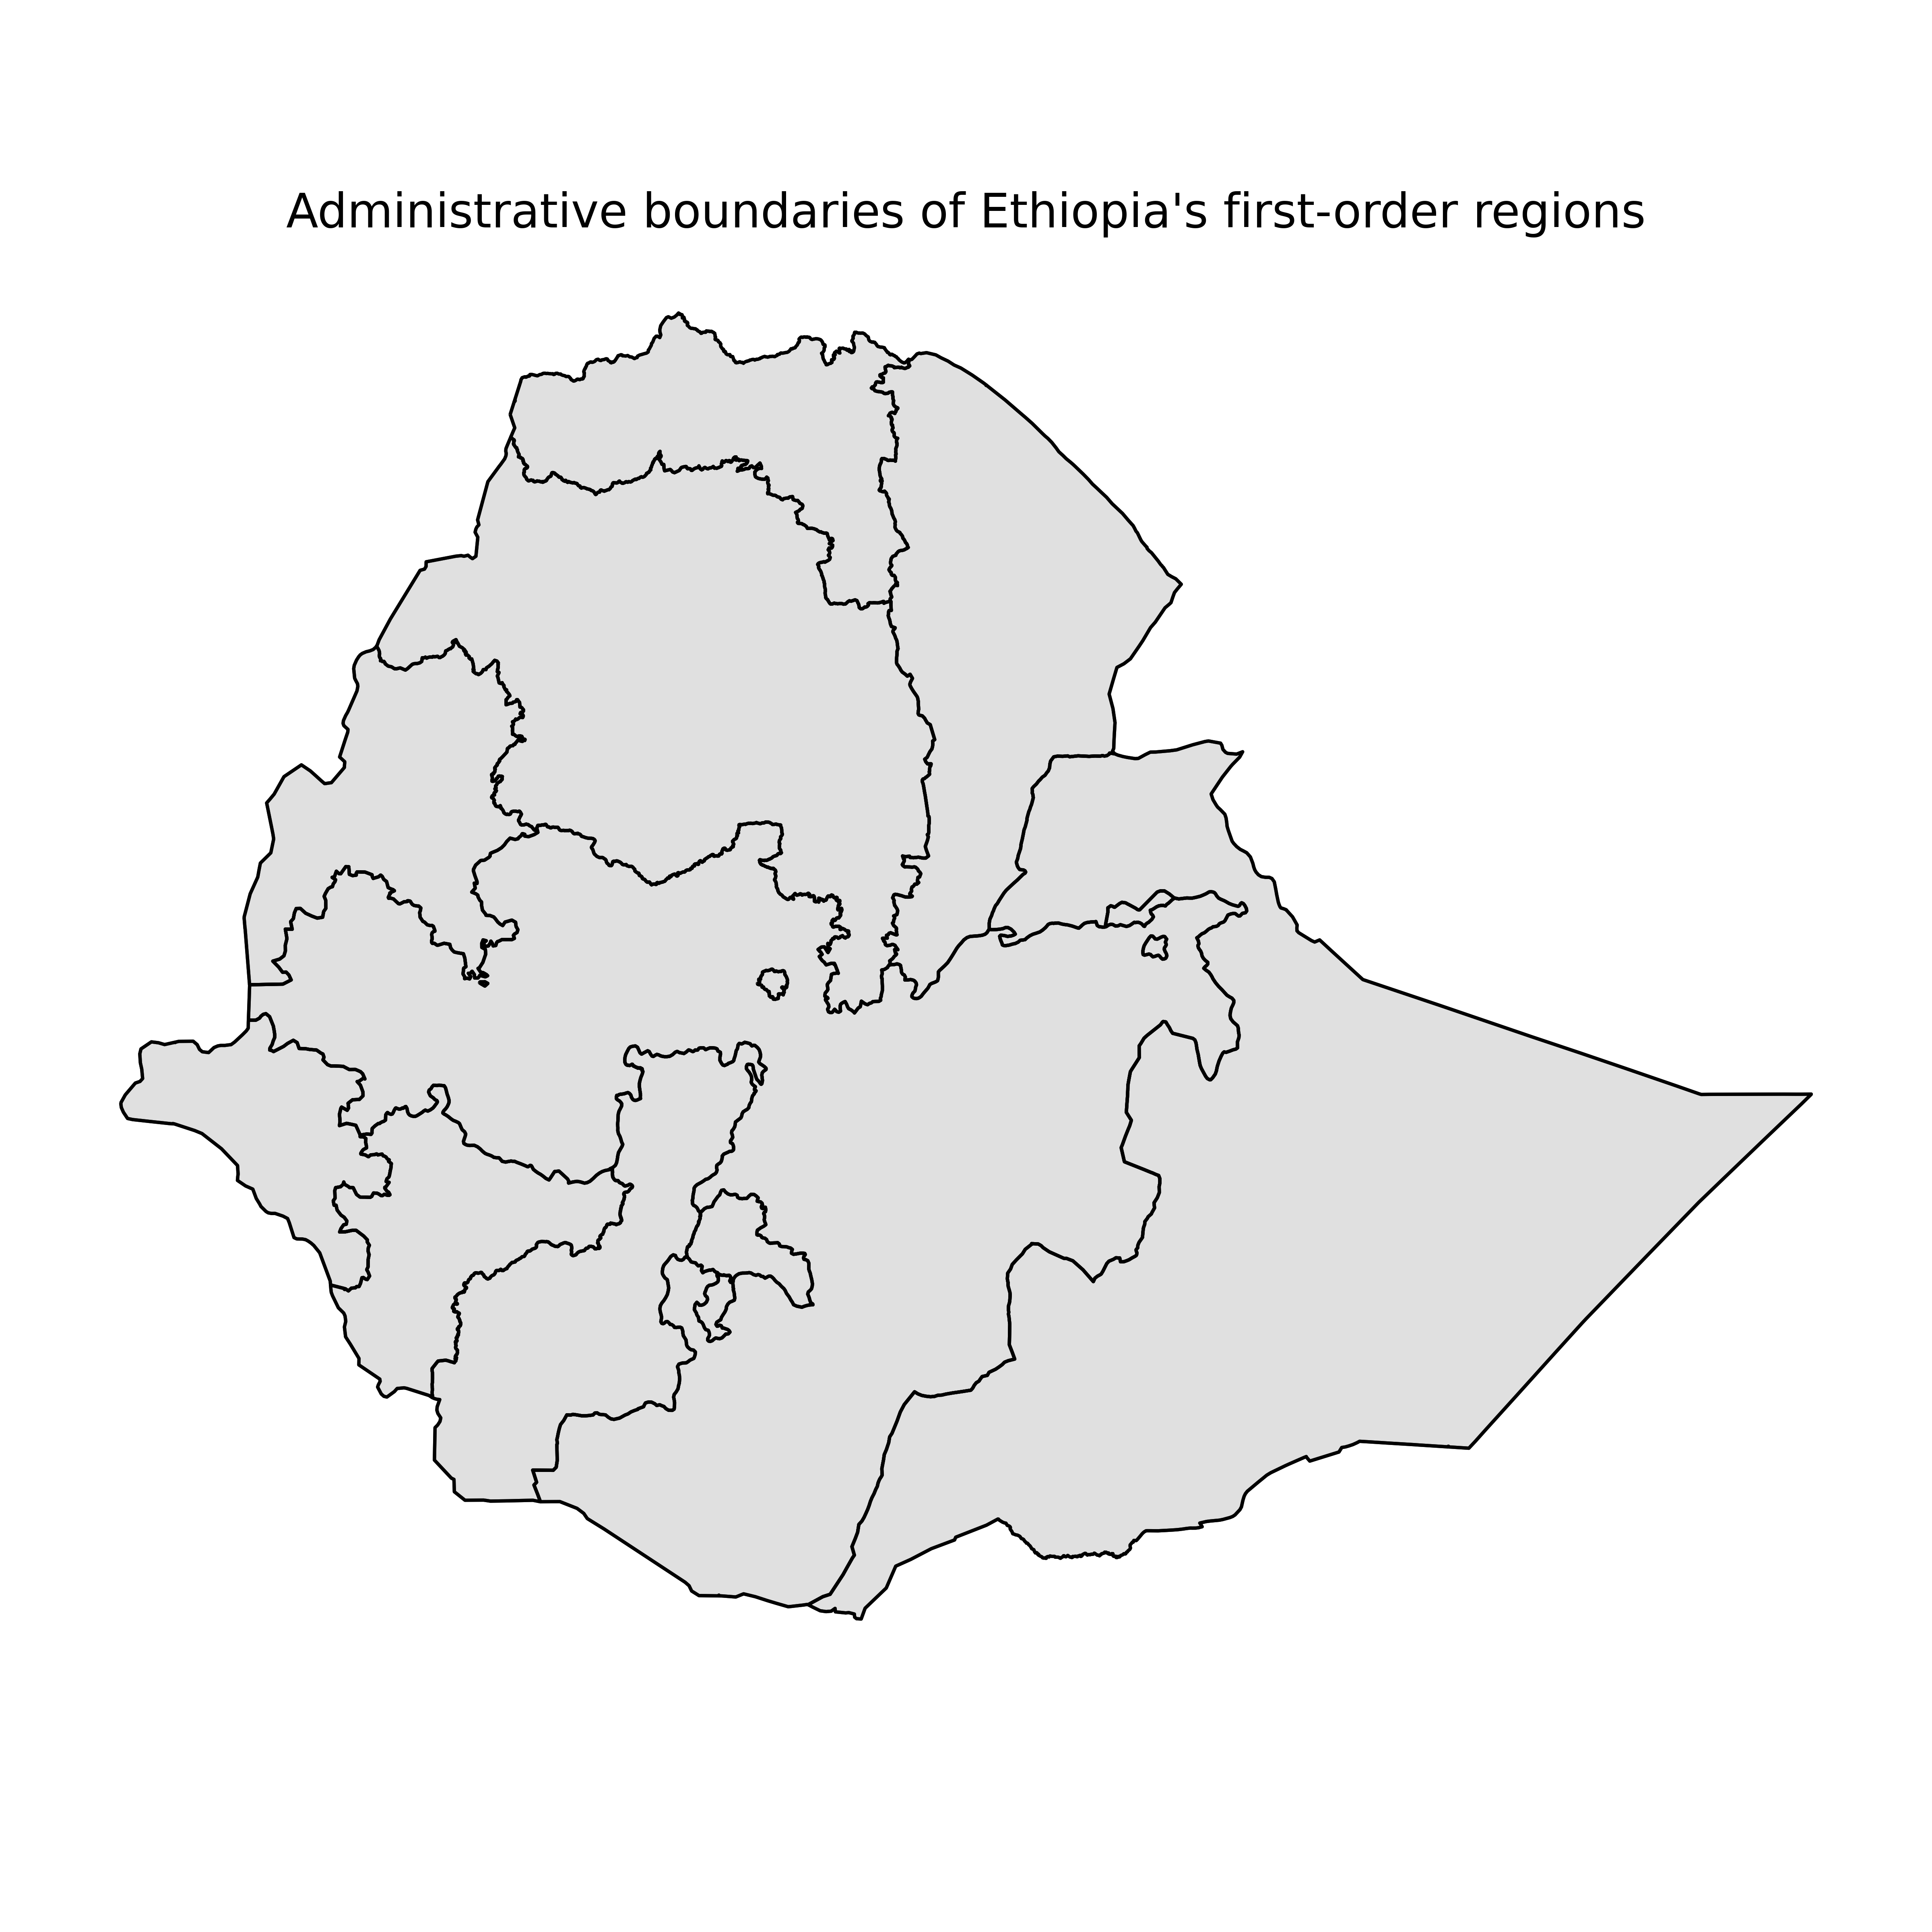
\includegraphics[width=0.7\textwidth]{outputs/figures/admin/ethiopia_admin_map.png}
	\caption{Administrative boundaries of Ethiopia's first-order regions. The map displays the 13 regional units used in the analysis, highlighting the evolving and fragmented nature of administrative boundaries over the study period.}
	\label{fig:admin_map}
\end{figure}
% --- End Figure 5 ---

\section{Identification Challenges in Small-N Panel Settings}

In empirical analyses of political favoritism using nighttime lights (NTL) data, identification is particularly challenging in settings with a small number of regions, limited exogenous variation in treatment, and high outcome concentration. This section outlines three core challenges that jointly limit inference in such panel data contexts.

\subsection{Omitted Variable Bias (without time fixed effects)}

When time fixed effects are omitted from panel regressions, estimates of leader-region favoritism are vulnerable to omitted variable bias. In the Ethiopian context, national economic shocks—such as booms or downturns—often coincide with leadership transitions. Without controlling for year effects, the estimated association between a leader’s birth region and regional luminosity may simply reflect these broader national trends, rather than any causal effect of political favoritism. Empirically, baseline models that exclude time fixed effects tend to produce inflated and statistically significant coefficients, but placebo tests and diagnostic plots reveal that these results are largely driven by common shocks rather than genuine treatment effects.

\subsection{Limited Identifying Variation (with time fixed effects)}

Including time fixed effects absorbs national shocks and common trends, but in small-N settings with few treated units and limited within-region, within-year variation, this approach introduces a new problem: limited identifying variation. When the timing of leader transitions is highly collinear with year effects, the model cannot reliably distinguish leader-region effects from national shocks. In the Ethiopian panel, the inclusion of time fixed effects sharply attenuates the estimated coefficients and increases standard errors, indicating that the available variation is insufficient for robust identification. The empirical p-values from placebo tests further confirm that observed effects are not distinguishable from random assignment.

\subsection{Low Statistical Power (small number of treated units)}

A third challenge is low statistical power, which arises from the small number of regions and limited number of leadership transitions. With only a handful of treated units and sparse treatment events, the effective sample size for identifying leader-region effects is severely constrained. This results in wide confidence intervals and imprecise estimates, particularly in event-study analyses and placebo simulations. The inability to detect dynamic effects or distinguish real from placebo results is a direct consequence of this low power, as demonstrated by the high empirical p-values and the overlap between observed and placebo distributions.

\paragraph{Synthesis}

Taken together, these challenges—omitted variable bias, limited identifying variation, and low statistical power—jointly undermine the credibility of causal inference in small-N panel settings. In the Ethiopian case, and in similar contexts, the combination of these factors means that apparent evidence for political favoritism is not empirically distinguishable from noise. Robust identification requires richer data, more exogenous variation, and careful diagnostic testing to avoid spurious findings.

\section{Literature Review}
This study sits at the intersection of three literatures.

First, a substantial literature uses satellite luminosity to measure economic activity. Early work established that light emissions track national and regional output surprisingly well in settings with limited conventional statistics \citep{Chen2011,Henderson2012}. More recent contributions show that the strength of this relationship varies with population density, sectoral composition, and spatial scale, which makes local interpretation more difficult than national validation exercises might suggest \citep{Bluhm2022,Gibson2021}. Work on harmonized long-run products has also improved the temporal comparability of DMSP-OLS and VIIRS series, but it has not eliminated measurement challenges \citep{Li2023,Gibson2024}.

Second, the paper relates to research on regional and ethnic favoritism. \citet{Hodler2014} show that political leaders' birth regions tend to receive higher nighttime light intensity in a broad cross-country sample. Subsequent work has refined that perspective by emphasizing the interaction between political favoritism, local ethnic demography, and institutions \citep{BeiserMcGrath2021}. Recent studies also continue to find geographically targeted favoritism in other settings, including public investment and local clientelism \citep{Onana2024,Cruzatti2024}. The implication is not that favoritism is universal, but that claims about it should be tested against within-unit changes rather than cross-sectional differences.




Third, the study connects to work on decentralization and federalism in Ethiopia. Existing scholarship highlights the tension between formal regional autonomy and persistent vertical control, including constraints on local fiscal autonomy and uneven developmental capacity \citep{Faguet2021,Wubneh2017}. Those institutional features make Ethiopia a theoretically important case for studying regional inequality, but they also heighten the need for careful empirical design. If regional trajectories differ for structural reasons unrelated to political leadership, pooled cross-sectional comparisons can easily be mistaken for favoritism.

\subsection*{Political Economy of Ethiopian Federalism}
The spatial distribution of rents in Ethiopia is deeply shaped by the country’s federal architecture and the political strategies of its ruling coalitions. Under the Ethiopian People’s Revolutionary Democratic Front (EPRDF), federalism was formally enshrined, but real power remained highly centralized. The EPRDF’s dominance over regional governments meant that resource allocation, investment, and development projects were often coordinated from the center, with regional administrations acting as agents rather than autonomous principals. This centralization is theorized to produce a spatial distribution of rents that is less responsive to local political dynamics and more reflective of national priorities and coalition management. In contrast, the current administration has presided over a period of greater regional contestation and, in some cases, increased regional autonomy. According to \citet{Faguet2021}, such shifts can alter the expected pattern of rent distribution: as regional governments gain more effective autonomy, the allocation of resources may become more sensitive to local political competition, ethnic demography, and the bargaining power of regional elites. This theoretical perspective suggests that the empirical analysis of favoritism in Ethiopia must account for changes in the structure of federalism and the evolving balance of power between center and regions.

Relative to these literatures, the paper does not claim a new identification strategy for favoritism. Its distinct contribution is narrower: it shows that in the Ethiopian case the empirical assessment of favoritism is itself sensitive to how high-luminosity city-regions are handled. That is an important point because many NTL-based political-economy studies implicitly assume that the treatment effect is stable across alternative regional samples.

\section{Methodology}
\subsection{Data}
\subsubsection{Nighttime light data}
The repository contains a harmonized annual NTL series built from DMSP-OLS and VIIRS raster products. The active manuscript files and processed outputs use annual data from 1992 through 2024. The underlying scripts reference the pixel-scale corrected nighttime light product of \citet{Li2023} and annual VIIRS composites derived by \citet{Elvidge2021}. Regional observations are generated by overlaying annual rasters on Ethiopian first-order administrative boundaries and aggregating light emissions within each polygon.

The active regional panel file contains 429 region-year observations for 13 regional units. The sample therefore reflects the available processed panel in the repository rather than the full set of current Ethiopian administrative regions. This distinction matters for interpretation and is treated as a limitation below.
% --- Begin Figure 5: Admin Map ---
\begin{figure}[ht]
	\centering
	% Replace the following line with the actual path to your admin map graphic
	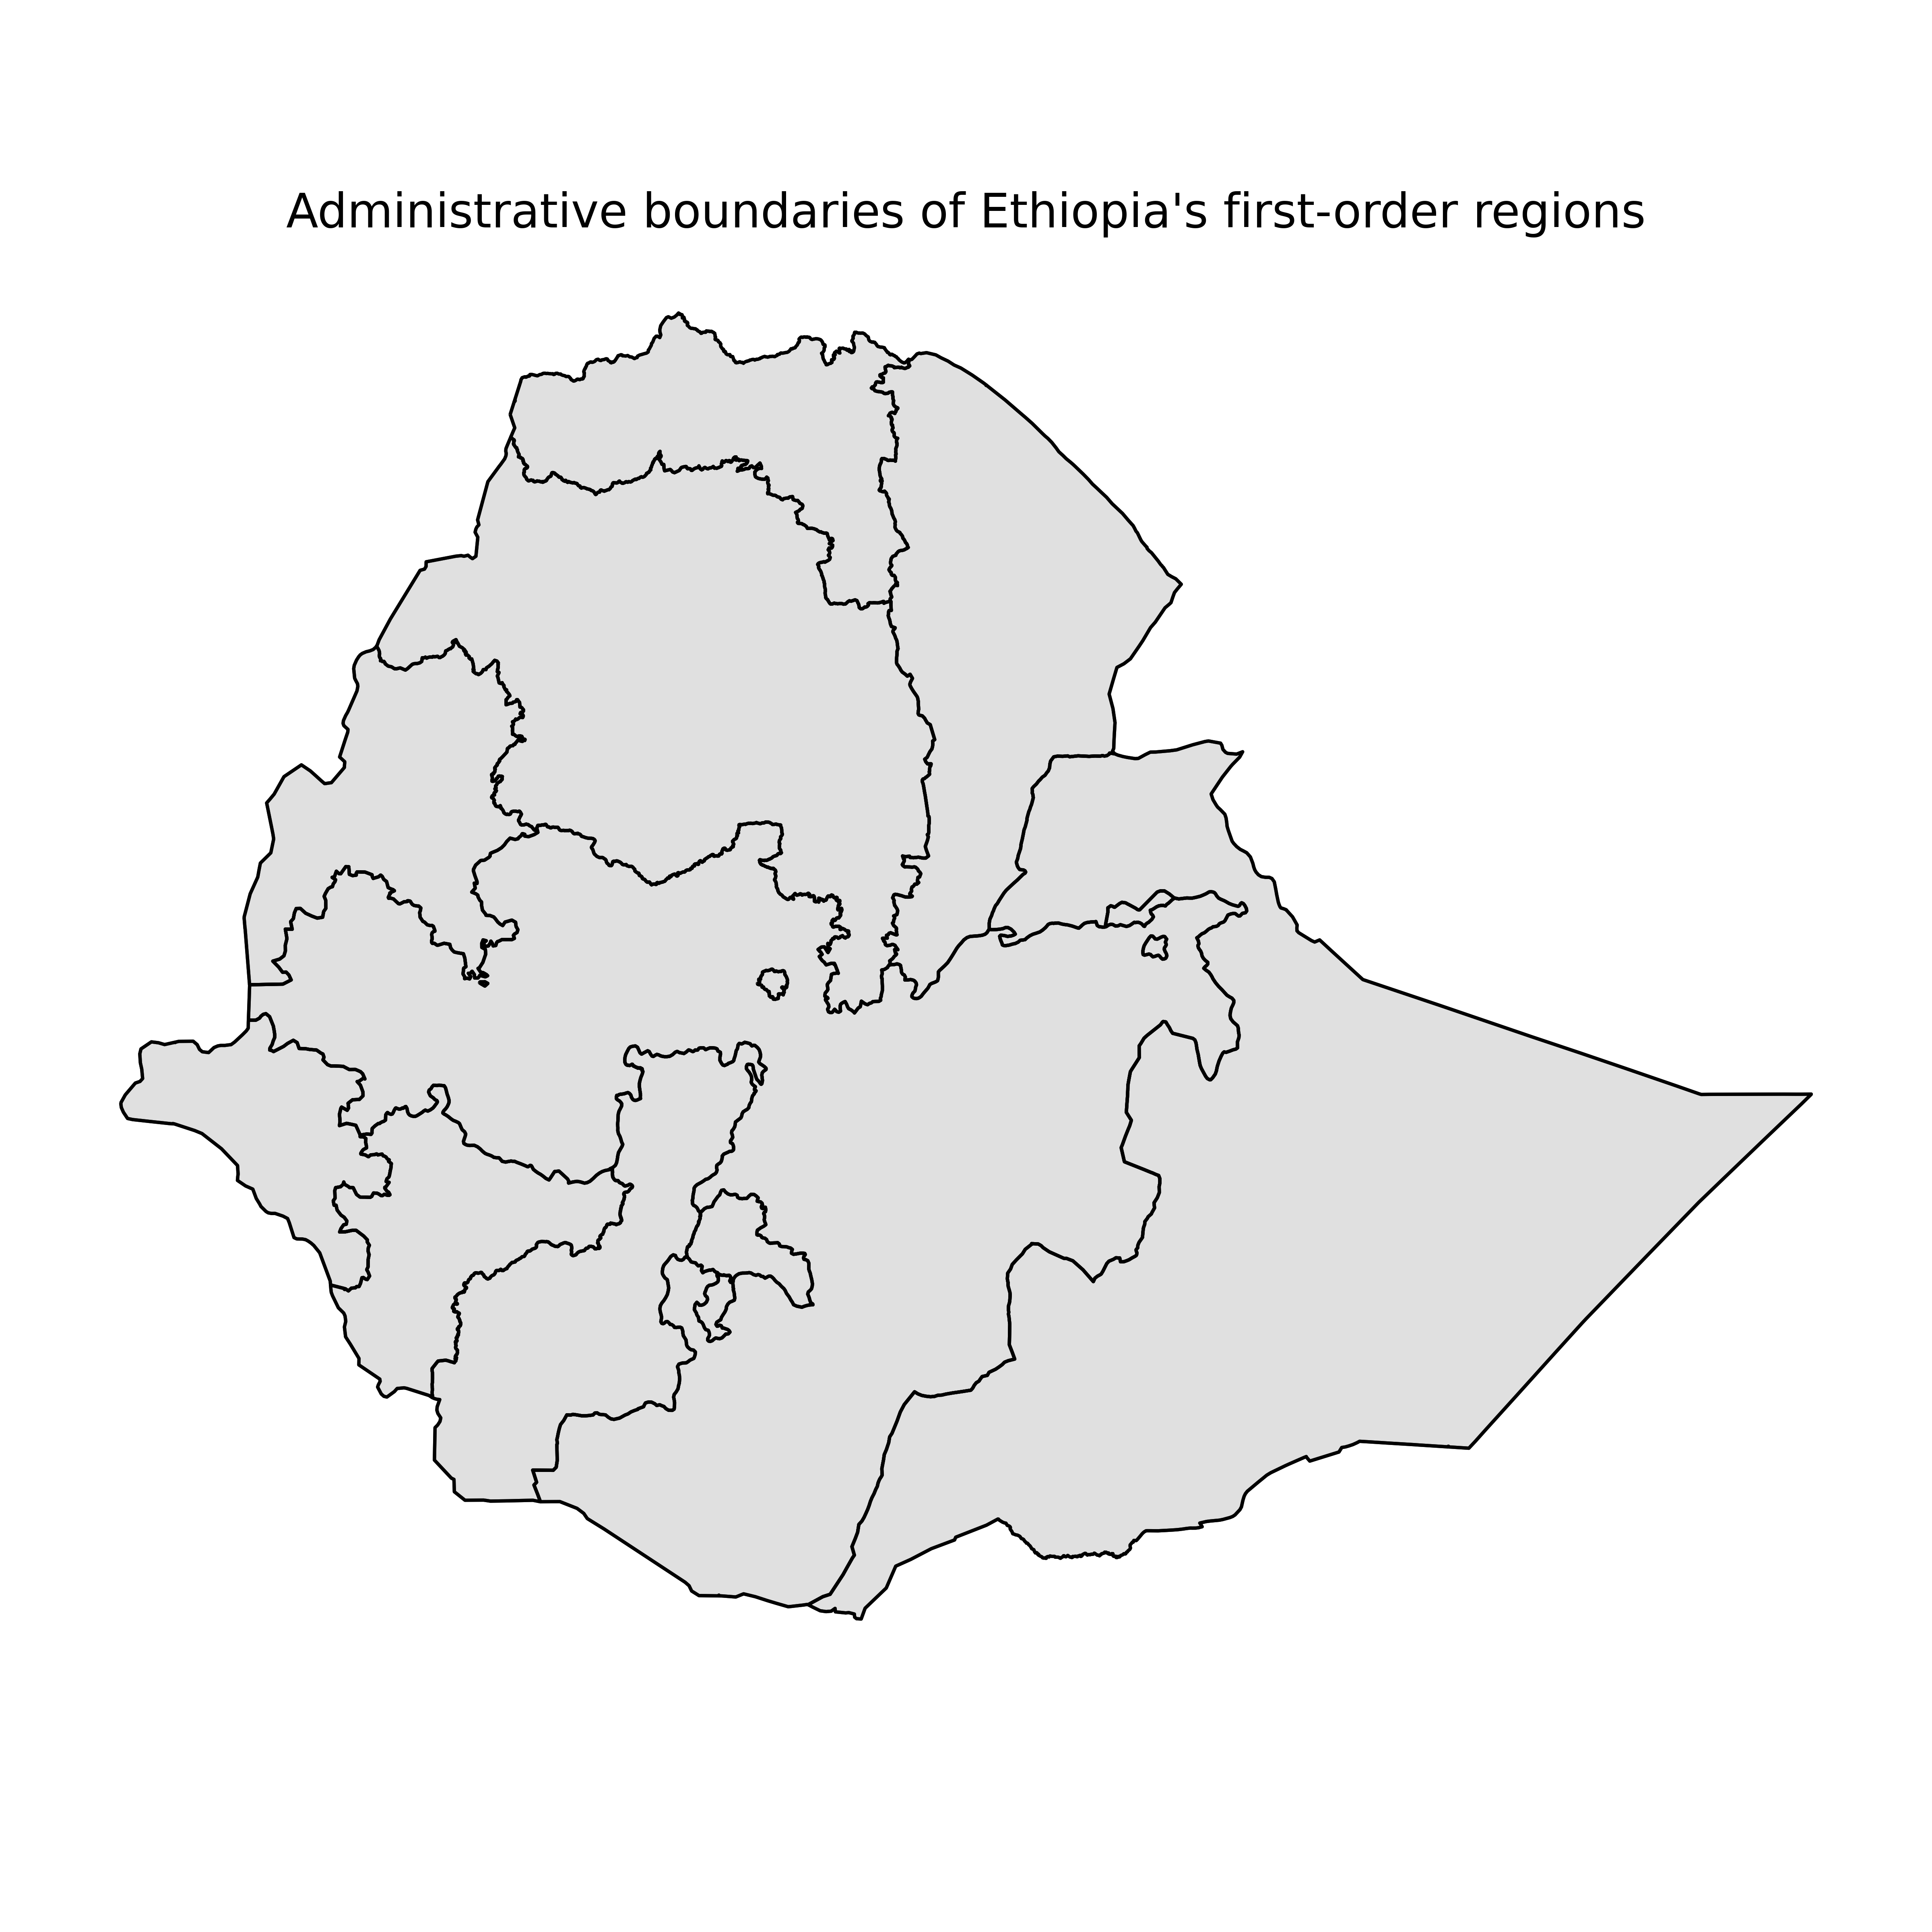
\includegraphics[width=0.7\textwidth]{outputs/figures/admin/ethiopia_admin_map.png}
	\caption{Administrative boundaries of Ethiopia's first-order regions. The map displays the 13 regional units used in the analysis, highlighting the evolving and fragmented nature of administrative boundaries over the study period.}
	\label{fig:admin_map}
\end{figure}
% --- End Figure 5 ---

\section{Identification Challenges in Small-N Panel Settings}

In empirical analyses of political favoritism using nighttime lights (NTL) data, identification is particularly challenging in settings with a small number of regions, limited exogenous variation in treatment, and high outcome concentration. This section outlines three core challenges that jointly limit inference in such panel data contexts.

\subsection{Omitted Variable Bias (without time fixed effects)}

When time fixed effects are omitted from panel regressions, estimates of leader-region favoritism are vulnerable to omitted variable bias. In the Ethiopian context, national economic shocks—such as booms or downturns—often coincide with leadership transitions. Without controlling for year effects, the estimated association between a leader’s birth region and regional luminosity may simply reflect these broader national trends, rather than any causal effect of political favoritism. Empirically, baseline models that exclude time fixed effects tend to produce inflated and statistically significant coefficients, but placebo tests and diagnostic plots reveal that these results are largely driven by common shocks rather than genuine treatment effects.

\subsection{Limited Identifying Variation (with time fixed effects)}

Including time fixed effects absorbs national shocks and common trends, but in small-N settings with few treated units and limited within-region, within-year variation, this approach introduces a new problem: limited identifying variation. When the timing of leader transitions is highly collinear with year effects, the model cannot reliably distinguish leader-region effects from national shocks. In the Ethiopian panel, the inclusion of time fixed effects sharply attenuates the estimated coefficients and increases standard errors, indicating that the available variation is insufficient for robust identification. The empirical p-values from placebo tests further confirm that observed effects are not distinguishable from random assignment.

\subsection{Low Statistical Power (small number of treated units)}

A third challenge is low statistical power, which arises from the small number of regions and limited number of leadership transitions. With only a handful of treated units and sparse treatment events, the effective sample size for identifying leader-region effects is severely constrained. This results in wide confidence intervals and imprecise estimates, particularly in event-study analyses and placebo simulations. The inability to detect dynamic effects or distinguish real from placebo results is a direct consequence of this low power, as demonstrated by the high empirical p-values and the overlap between observed and placebo distributions.

\paragraph{Synthesis}

Taken together, these challenges—omitted variable bias, limited identifying variation, and low statistical power—jointly undermine the credibility of causal inference in small-N panel settings. In the Ethiopian case, and in similar contexts, the combination of these factors means that apparent evidence for political favoritism is not empirically distinguishable from noise. Robust identification requires richer data, more exogenous variation, and careful diagnostic testing to avoid spurious findings.

\section{Literature Review}
This study sits at the intersection of three literatures.

First, a substantial literature uses satellite luminosity to measure economic activity. Early work established that light emissions track national and regional output surprisingly well in settings with limited conventional statistics \citep{Chen2011,Henderson2012}. More recent contributions show that the strength of this relationship varies with population density, sectoral composition, and spatial scale, which makes local interpretation more difficult than national validation exercises might suggest \citep{Bluhm2022,Gibson2021}. Work on harmonized long-run products has also improved the temporal comparability of DMSP-OLS and VIIRS series, but it has not eliminated measurement challenges \citep{Li2023,Gibson2024}.

Second, the paper relates to research on regional and ethnic favoritism. \citet{Hodler2014} show that political leaders' birth regions tend to receive higher nighttime light intensity in a broad cross-country sample. Subsequent work has refined that perspective by emphasizing the interaction between political favoritism, local ethnic demography, and institutions \citep{BeiserMcGrath2021}. Recent studies also continue to find geographically targeted favoritism in other settings, including public investment and local clientelism \citep{Onana2024,Cruzatti2024}. The implication is not that favoritism is universal, but that claims about it should be tested against within-unit changes rather than cross-sectional differences.




Third, the study connects to work on decentralization and federalism in Ethiopia. Existing scholarship highlights the tension between formal regional autonomy and persistent vertical control, including constraints on local fiscal autonomy and uneven developmental capacity \citep{Faguet2021,Wubneh2017}. Those institutional features make Ethiopia a theoretically important case for studying regional inequality, but they also heighten the need for careful empirical design. If regional trajectories differ for structural reasons unrelated to political leadership, pooled cross-sectional comparisons can easily be mistaken for favoritism.

\subsection*{Political Economy of Ethiopian Federalism}
The spatial distribution of rents in Ethiopia is deeply shaped by the country’s federal architecture and the political strategies of its ruling coalitions. Under the Ethiopian People’s Revolutionary Democratic Front (EPRDF), federalism was formally enshrined, but real power remained highly centralized. The EPRDF’s dominance over regional governments meant that resource allocation, investment, and development projects were often coordinated from the center, with regional administrations acting as agents rather than autonomous principals. This centralization is theorized to produce a spatial distribution of rents that is less responsive to local political dynamics and more reflective of national priorities and coalition management. In contrast, the current administration has presided over a period of greater regional contestation and, in some cases, increased regional autonomy. According to \citet{Faguet2021}, such shifts can alter the expected pattern of rent distribution: as regional governments gain more effective autonomy, the allocation of resources may become more sensitive to local political competition, ethnic demography, and the bargaining power of regional elites. This theoretical perspective suggests that the empirical analysis of favoritism in Ethiopia must account for changes in the structure of federalism and the evolving balance of power between center and regions.

Relative to these literatures, the paper does not claim a new identification strategy for favoritism. Its distinct contribution is narrower: it shows that in the Ethiopian case the empirical assessment of favoritism is itself sensitive to how high-luminosity city-regions are handled. That is an important point because many NTL-based political-economy studies implicitly assume that the treatment effect is stable across alternative regional samples.

\section{Methodology}
\subsection{Data}
\subsubsection{Nighttime light data}
The repository contains a harmonized annual NTL series built from DMSP-OLS and VIIRS raster products. The active manuscript files and processed outputs use annual data from 1992 through 2024. The underlying scripts reference the pixel-scale corrected nighttime light product of \citet{Li2023} and annual VIIRS composites derived by \citet{Elvidge2021}. Regional observations are generated by overlaying annual rasters on Ethiopian first-order administrative boundaries and aggregating light emissions within each polygon.

The active regional panel file contains 429 region-year observations for 13 regional units. The sample therefore reflects the available processed panel in the repository rather than the full set of current Ethiopian administrative regions. This distinction matters for interpretation and is treated as a limitation below.
% --- Begin Figure 5: Admin Map ---
\begin{figure}[ht]
	\centering
	% Replace the following line with the actual path to your admin map graphic
	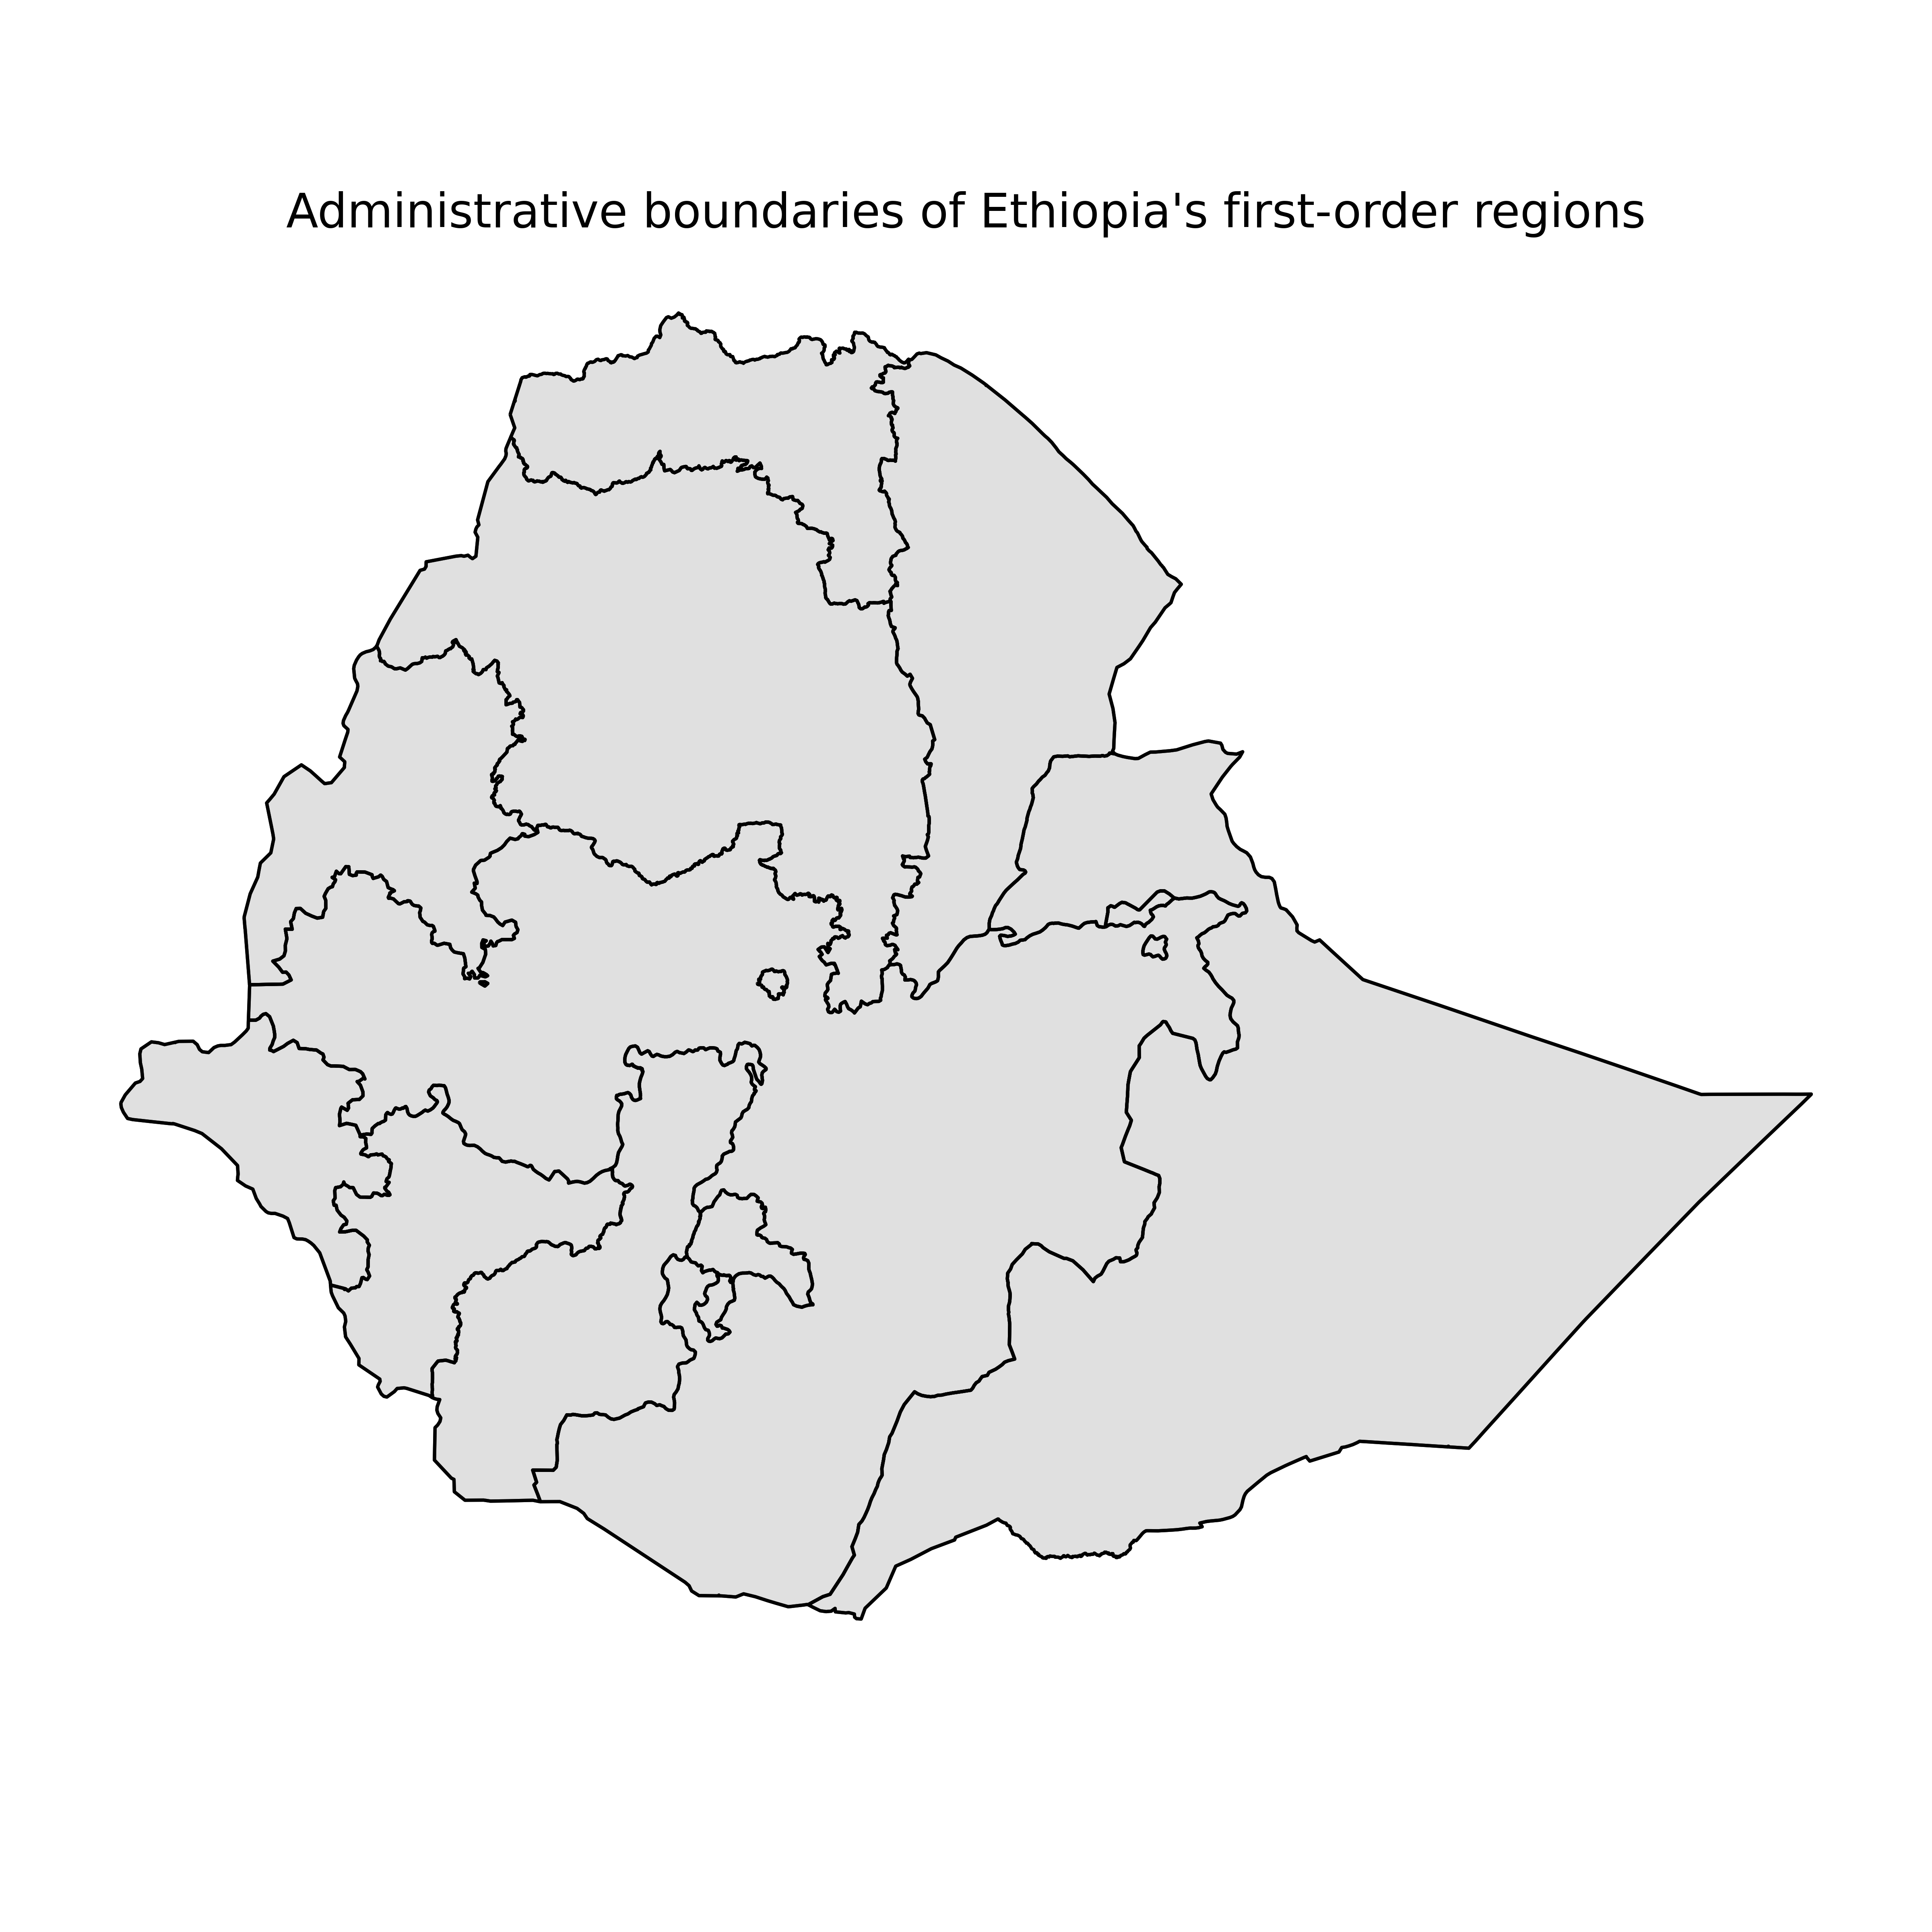
\includegraphics[width=0.7\textwidth]{outputs/figures/admin/ethiopia_admin_map.png}
	\caption{Administrative boundaries of Ethiopia's first-order regions. The map displays the 13 regional units used in the analysis, highlighting the evolving and fragmented nature of administrative boundaries over the study period.}
	\label{fig:admin_map}
\end{figure}
% --- End Figure 5 ---

\section{Identification Challenges in Small-N Panel Settings}

In empirical analyses of political favoritism using nighttime lights (NTL) data, identification is particularly challenging in settings with a small number of regions, limited exogenous variation in treatment, and high outcome concentration. This section outlines three core challenges that jointly limit inference in such panel data contexts.

\subsection{Omitted Variable Bias (without time fixed effects)}

When time fixed effects are omitted from panel regressions, estimates of leader-region favoritism are vulnerable to omitted variable bias. In the Ethiopian context, national economic shocks—such as booms or downturns—often coincide with leadership transitions. Without controlling for year effects, the estimated association between a leader’s birth region and regional luminosity may simply reflect these broader national trends, rather than any causal effect of political favoritism. Empirically, baseline models that exclude time fixed effects tend to produce inflated and statistically significant coefficients, but placebo tests and diagnostic plots reveal that these results are largely driven by common shocks rather than genuine treatment effects.

\subsection{Limited Identifying Variation (with time fixed effects)}

Including time fixed effects absorbs national shocks and common trends, but in small-N settings with few treated units and limited within-region, within-year variation, this approach introduces a new problem: limited identifying variation. When the timing of leader transitions is highly collinear with year effects, the model cannot reliably distinguish leader-region effects from national shocks. In the Ethiopian panel, the inclusion of time fixed effects sharply attenuates the estimated coefficients and increases standard errors, indicating that the available variation is insufficient for robust identification. The empirical p-values from placebo tests further confirm that observed effects are not distinguishable from random assignment.

\subsection{Low Statistical Power (small number of treated units)}

A third challenge is low statistical power, which arises from the small number of regions and limited number of leadership transitions. With only a handful of treated units and sparse treatment events, the effective sample size for identifying leader-region effects is severely constrained. This results in wide confidence intervals and imprecise estimates, particularly in event-study analyses and placebo simulations. The inability to detect dynamic effects or distinguish real from placebo results is a direct consequence of this low power, as demonstrated by the high empirical p-values and the overlap between observed and placebo distributions.

\paragraph{Synthesis}

Taken together, these challenges—omitted variable bias, limited identifying variation, and low statistical power—jointly undermine the credibility of causal inference in small-N panel settings. In the Ethiopian case, and in similar contexts, the combination of these factors means that apparent evidence for political favoritism is not empirically distinguishable from noise. Robust identification requires richer data, more exogenous variation, and careful diagnostic testing to avoid spurious findings.

\section{Literature Review}
This study sits at the intersection of three literatures.

First, a substantial literature uses satellite luminosity to measure economic activity. Early work established that light emissions track national and regional output surprisingly well in settings with limited conventional statistics \citep{Chen2011,Henderson2012}. More recent contributions show that the strength of this relationship varies with population density, sectoral composition, and spatial scale, which makes local interpretation more difficult than national validation exercises might suggest \citep{Bluhm2022,Gibson2021}. Work on harmonized long-run products has also improved the temporal comparability of DMSP-OLS and VIIRS series, but it has not eliminated measurement challenges \citep{Li2023,Gibson2024}.

Second, the paper relates to research on regional and ethnic favoritism. \citet{Hodler2014} show that political leaders' birth regions tend to receive higher nighttime light intensity in a broad cross-country sample. Subsequent work has refined that perspective by emphasizing the interaction between political favoritism, local ethnic demography, and institutions \citep{BeiserMcGrath2021}. Recent studies also continue to find geographically targeted favoritism in other settings, including public investment and local clientelism \citep{Onana2024,Cruzatti2024}. The implication is not that favoritism is universal, but that claims about it should be tested against within-unit changes rather than cross-sectional differences.




Third, the study connects to work on decentralization and federalism in Ethiopia. Existing scholarship highlights the tension between formal regional autonomy and persistent vertical control, including constraints on local fiscal autonomy and uneven developmental capacity \citep{Faguet2021,Wubneh2017}. Those institutional features make Ethiopia a theoretically important case for studying regional inequality, but they also heighten the need for careful empirical design. If regional trajectories differ for structural reasons unrelated to political leadership, pooled cross-sectional comparisons can easily be mistaken for favoritism.

\subsection*{Political Economy of Ethiopian Federalism}
The spatial distribution of rents in Ethiopia is deeply shaped by the country’s federal architecture and the political strategies of its ruling coalitions. Under the Ethiopian People’s Revolutionary Democratic Front (EPRDF), federalism was formally enshrined, but real power remained highly centralized. The EPRDF’s dominance over regional governments meant that resource allocation, investment, and development projects were often coordinated from the center, with regional administrations acting as agents rather than autonomous principals. This centralization is theorized to produce a spatial distribution of rents that is less responsive to local political dynamics and more reflective of national priorities and coalition management. In contrast, the current administration has presided over a period of greater regional contestation and, in some cases, increased regional autonomy. According to \citet{Faguet2021}, such shifts can alter the expected pattern of rent distribution: as regional governments gain more effective autonomy, the allocation of resources may become more sensitive to local political competition, ethnic demography, and the bargaining power of regional elites. This theoretical perspective suggests that the empirical analysis of favoritism in Ethiopia must account for changes in the structure of federalism and the evolving balance of power between center and regions.

Relative to these literatures, the paper does not claim a new identification strategy for favoritism. Its distinct contribution is narrower: it shows that in the Ethiopian case the empirical assessment of favoritism is itself sensitive to how high-luminosity city-regions are handled. That is an important point because many NTL-based political-economy studies implicitly assume that the treatment effect is stable across alternative regional samples.

\section{Methodology}
\subsection{Data}
\subsubsection{Nighttime light data}
The repository contains a harmonized annual NTL series built from DMSP-OLS and VIIRS raster products. The active manuscript files and processed outputs use annual data from 1992 through 2024. The underlying scripts reference the pixel-scale corrected nighttime light product of \citet{Li2023} and annual VIIRS composites derived by \citet{Elvidge2021}. Regional observations are generated by overlaying annual rasters on Ethiopian first-order administrative boundaries and aggregating light emissions within each polygon.

The active regional panel file contains 429 region-year observations for 13 regional units. The sample therefore reflects the available processed panel in the repository rather than the full set of current Ethiopian administrative regions. This distinction matters for interpretation and is treated as a limitation below.
% --- Begin Figure 5: Admin Map ---
\begin{figure}[ht]
	\centering
	% Replace the following line with the actual path to your admin map graphic
	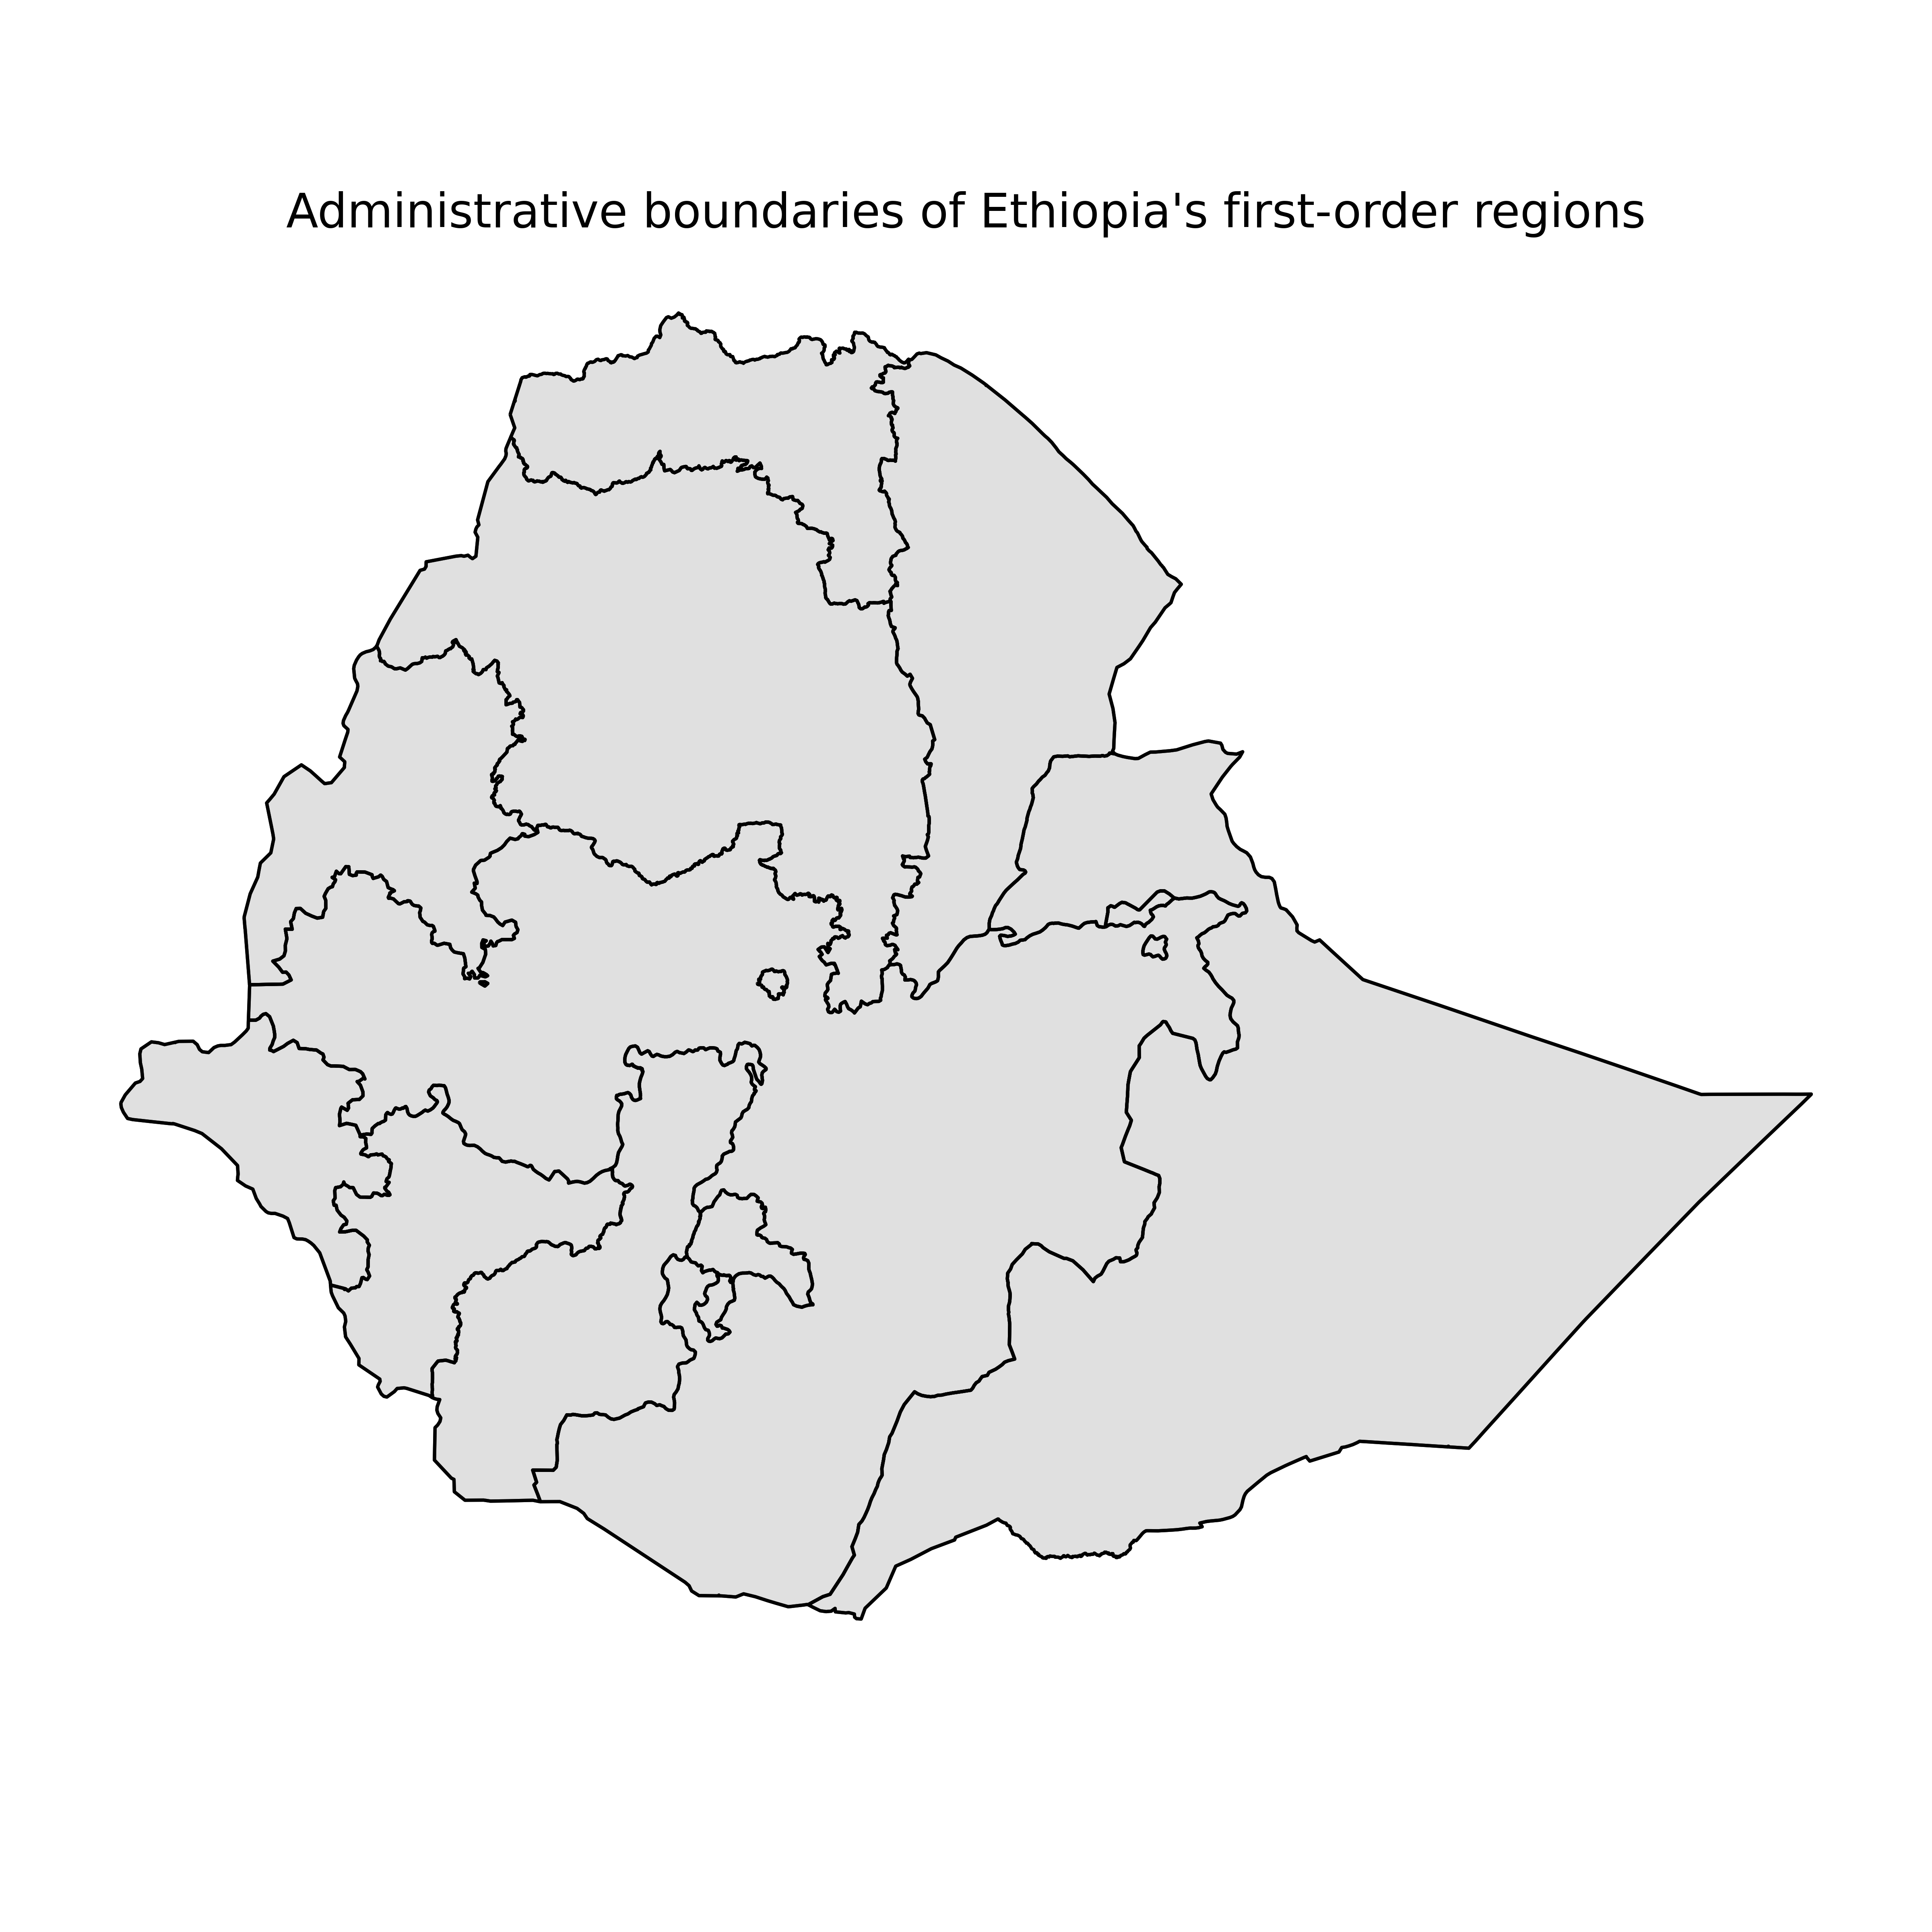
\includegraphics[width=0.7\textwidth]{outputs/figures/admin/ethiopia_admin_map.png}
	\caption{Administrative boundaries of Ethiopia's first-order regions. The map displays the 13 regional units used in the analysis, highlighting the evolving and fragmented nature of administrative boundaries over the study period.}
	\label{fig:admin_map}
\end{figure}
% --- End Figure 5 ---

\section{Identification Challenges in Small-N Panel Settings}

In empirical analyses of political favoritism using nighttime lights (NTL) data, identification is particularly challenging in settings with a small number of regions, limited exogenous variation in treatment, and high outcome concentration. This section outlines three core challenges that jointly limit inference in such panel data contexts.

\subsection{Omitted Variable Bias (without time fixed effects)}

When time fixed effects are omitted from panel regressions, estimates of leader-region favoritism are vulnerable to omitted variable bias. In the Ethiopian context, national economic shocks—such as booms or downturns—often coincide with leadership transitions. Without controlling for year effects, the estimated association between a leader’s birth region and regional luminosity may simply reflect these broader national trends, rather than any causal effect of political favoritism. Empirically, baseline models that exclude time fixed effects tend to produce inflated and statistically significant coefficients, but placebo tests and diagnostic plots reveal that these results are largely driven by common shocks rather than genuine treatment effects.

\subsection{Limited Identifying Variation (with time fixed effects)}

Including time fixed effects absorbs national shocks and common trends, but in small-N settings with few treated units and limited within-region, within-year variation, this approach introduces a new problem: limited identifying variation. When the timing of leader transitions is highly collinear with year effects, the model cannot reliably distinguish leader-region effects from national shocks. In the Ethiopian panel, the inclusion of time fixed effects sharply attenuates the estimated coefficients and increases standard errors, indicating that the available variation is insufficient for robust identification. The empirical p-values from placebo tests further confirm that observed effects are not distinguishable from random assignment.

\subsection{Low Statistical Power (small number of treated units)}

A third challenge is low statistical power, which arises from the small number of regions and limited number of leadership transitions. With only a handful of treated units and sparse treatment events, the effective sample size for identifying leader-region effects is severely constrained. This results in wide confidence intervals and imprecise estimates, particularly in event-study analyses and placebo simulations. The inability to detect dynamic effects or distinguish real from placebo results is a direct consequence of this low power, as demonstrated by the high empirical p-values and the overlap between observed and placebo distributions.

\paragraph{Synthesis}

Taken together, these challenges—omitted variable bias, limited identifying variation, and low statistical power—jointly undermine the credibility of causal inference in small-N panel settings. In the Ethiopian case, and in similar contexts, the combination of these factors means that apparent evidence for political favoritism is not empirically distinguishable from noise. Robust identification requires richer data, more exogenous variation, and careful diagnostic testing to avoid spurious findings.

\section{Literature Review}
This study sits at the intersection of three literatures.

First, a substantial literature uses satellite luminosity to measure economic activity. Early work established that light emissions track national and regional output surprisingly well in settings with limited conventional statistics \citep{Chen2011,Henderson2012}. More recent contributions show that the strength of this relationship varies with population density, sectoral composition, and spatial scale, which makes local interpretation more difficult than national validation exercises might suggest \citep{Bluhm2022,Gibson2021}. Work on harmonized long-run products has also improved the temporal comparability of DMSP-OLS and VIIRS series, but it has not eliminated measurement challenges \citep{Li2023,Gibson2024}.

Second, the paper relates to research on regional and ethnic favoritism. \citet{Hodler2014} show that political leaders' birth regions tend to receive higher nighttime light intensity in a broad cross-country sample. Subsequent work has refined that perspective by emphasizing the interaction between political favoritism, local ethnic demography, and institutions \citep{BeiserMcGrath2021}. Recent studies also continue to find geographically targeted favoritism in other settings, including public investment and local clientelism \citep{Onana2024,Cruzatti2024}. The implication is not that favoritism is universal, but that claims about it should be tested against within-unit changes rather than cross-sectional differences.




Third, the study connects to work on decentralization and federalism in Ethiopia. Existing scholarship highlights the tension between formal regional autonomy and persistent vertical control, including constraints on local fiscal autonomy and uneven developmental capacity \citep{Faguet2021,Wubneh2017}. Those institutional features make Ethiopia a theoretically important case for studying regional inequality, but they also heighten the need for careful empirical design. If regional trajectories differ for structural reasons unrelated to political leadership, pooled cross-sectional comparisons can easily be mistaken for favoritism.

\subsection*{Political Economy of Ethiopian Federalism}
The spatial distribution of rents in Ethiopia is deeply shaped by the country’s federal architecture and the political strategies of its ruling coalitions. Under the Ethiopian People’s Revolutionary Democratic Front (EPRDF), federalism was formally enshrined, but real power remained highly centralized. The EPRDF’s dominance over regional governments meant that resource allocation, investment, and development projects were often coordinated from the center, with regional administrations acting as agents rather than autonomous principals. This centralization is theorized to produce a spatial distribution of rents that is less responsive to local political dynamics and more reflective of national priorities and coalition management. In contrast, the current administration has presided over a period of greater regional contestation and, in some cases, increased regional autonomy. According to \citet{Faguet2021}, such shifts can alter the expected pattern of rent distribution: as regional governments gain more effective autonomy, the allocation of resources may become more sensitive to local political competition, ethnic demography, and the bargaining power of regional elites. This theoretical perspective suggests that the empirical analysis of favoritism in Ethiopia must account for changes in the structure of federalism and the evolving balance of power between center and regions.

Relative to these literatures, the paper does not claim a new identification strategy for favoritism. Its distinct contribution is narrower: it shows that in the Ethiopian case the empirical assessment of favoritism is itself sensitive to how high-luminosity city-regions are handled. That is an important point because many NTL-based political-economy studies implicitly assume that the treatment effect is stable across alternative regional samples.

\section{Methodology}
\subsection{Data}
\subsubsection{Nighttime light data}
The repository contains a harmonized annual NTL series built from DMSP-OLS and VIIRS raster products. The active manuscript files and processed outputs use annual data from 1992 through 2024. The underlying scripts reference the pixel-scale corrected nighttime light product of \citet{Li2023} and annual VIIRS composites derived by \citet{Elvidge2021}. Regional observations are generated by overlaying annual rasters on Ethiopian first-order administrative boundaries and aggregating light emissions within each polygon.

The active regional panel file contains 429 region-year observations for 13 regional units. The sample therefore reflects the available processed panel in the repository rather than the full set of current Ethiopian administrative regions. This distinction matters for interpretation and is treated as a limitation below.
% --- Begin Figure 5: Admin Map ---
\begin{figure}[ht]
	\centering
	% Replace the following line with the actual path to your admin map graphic
	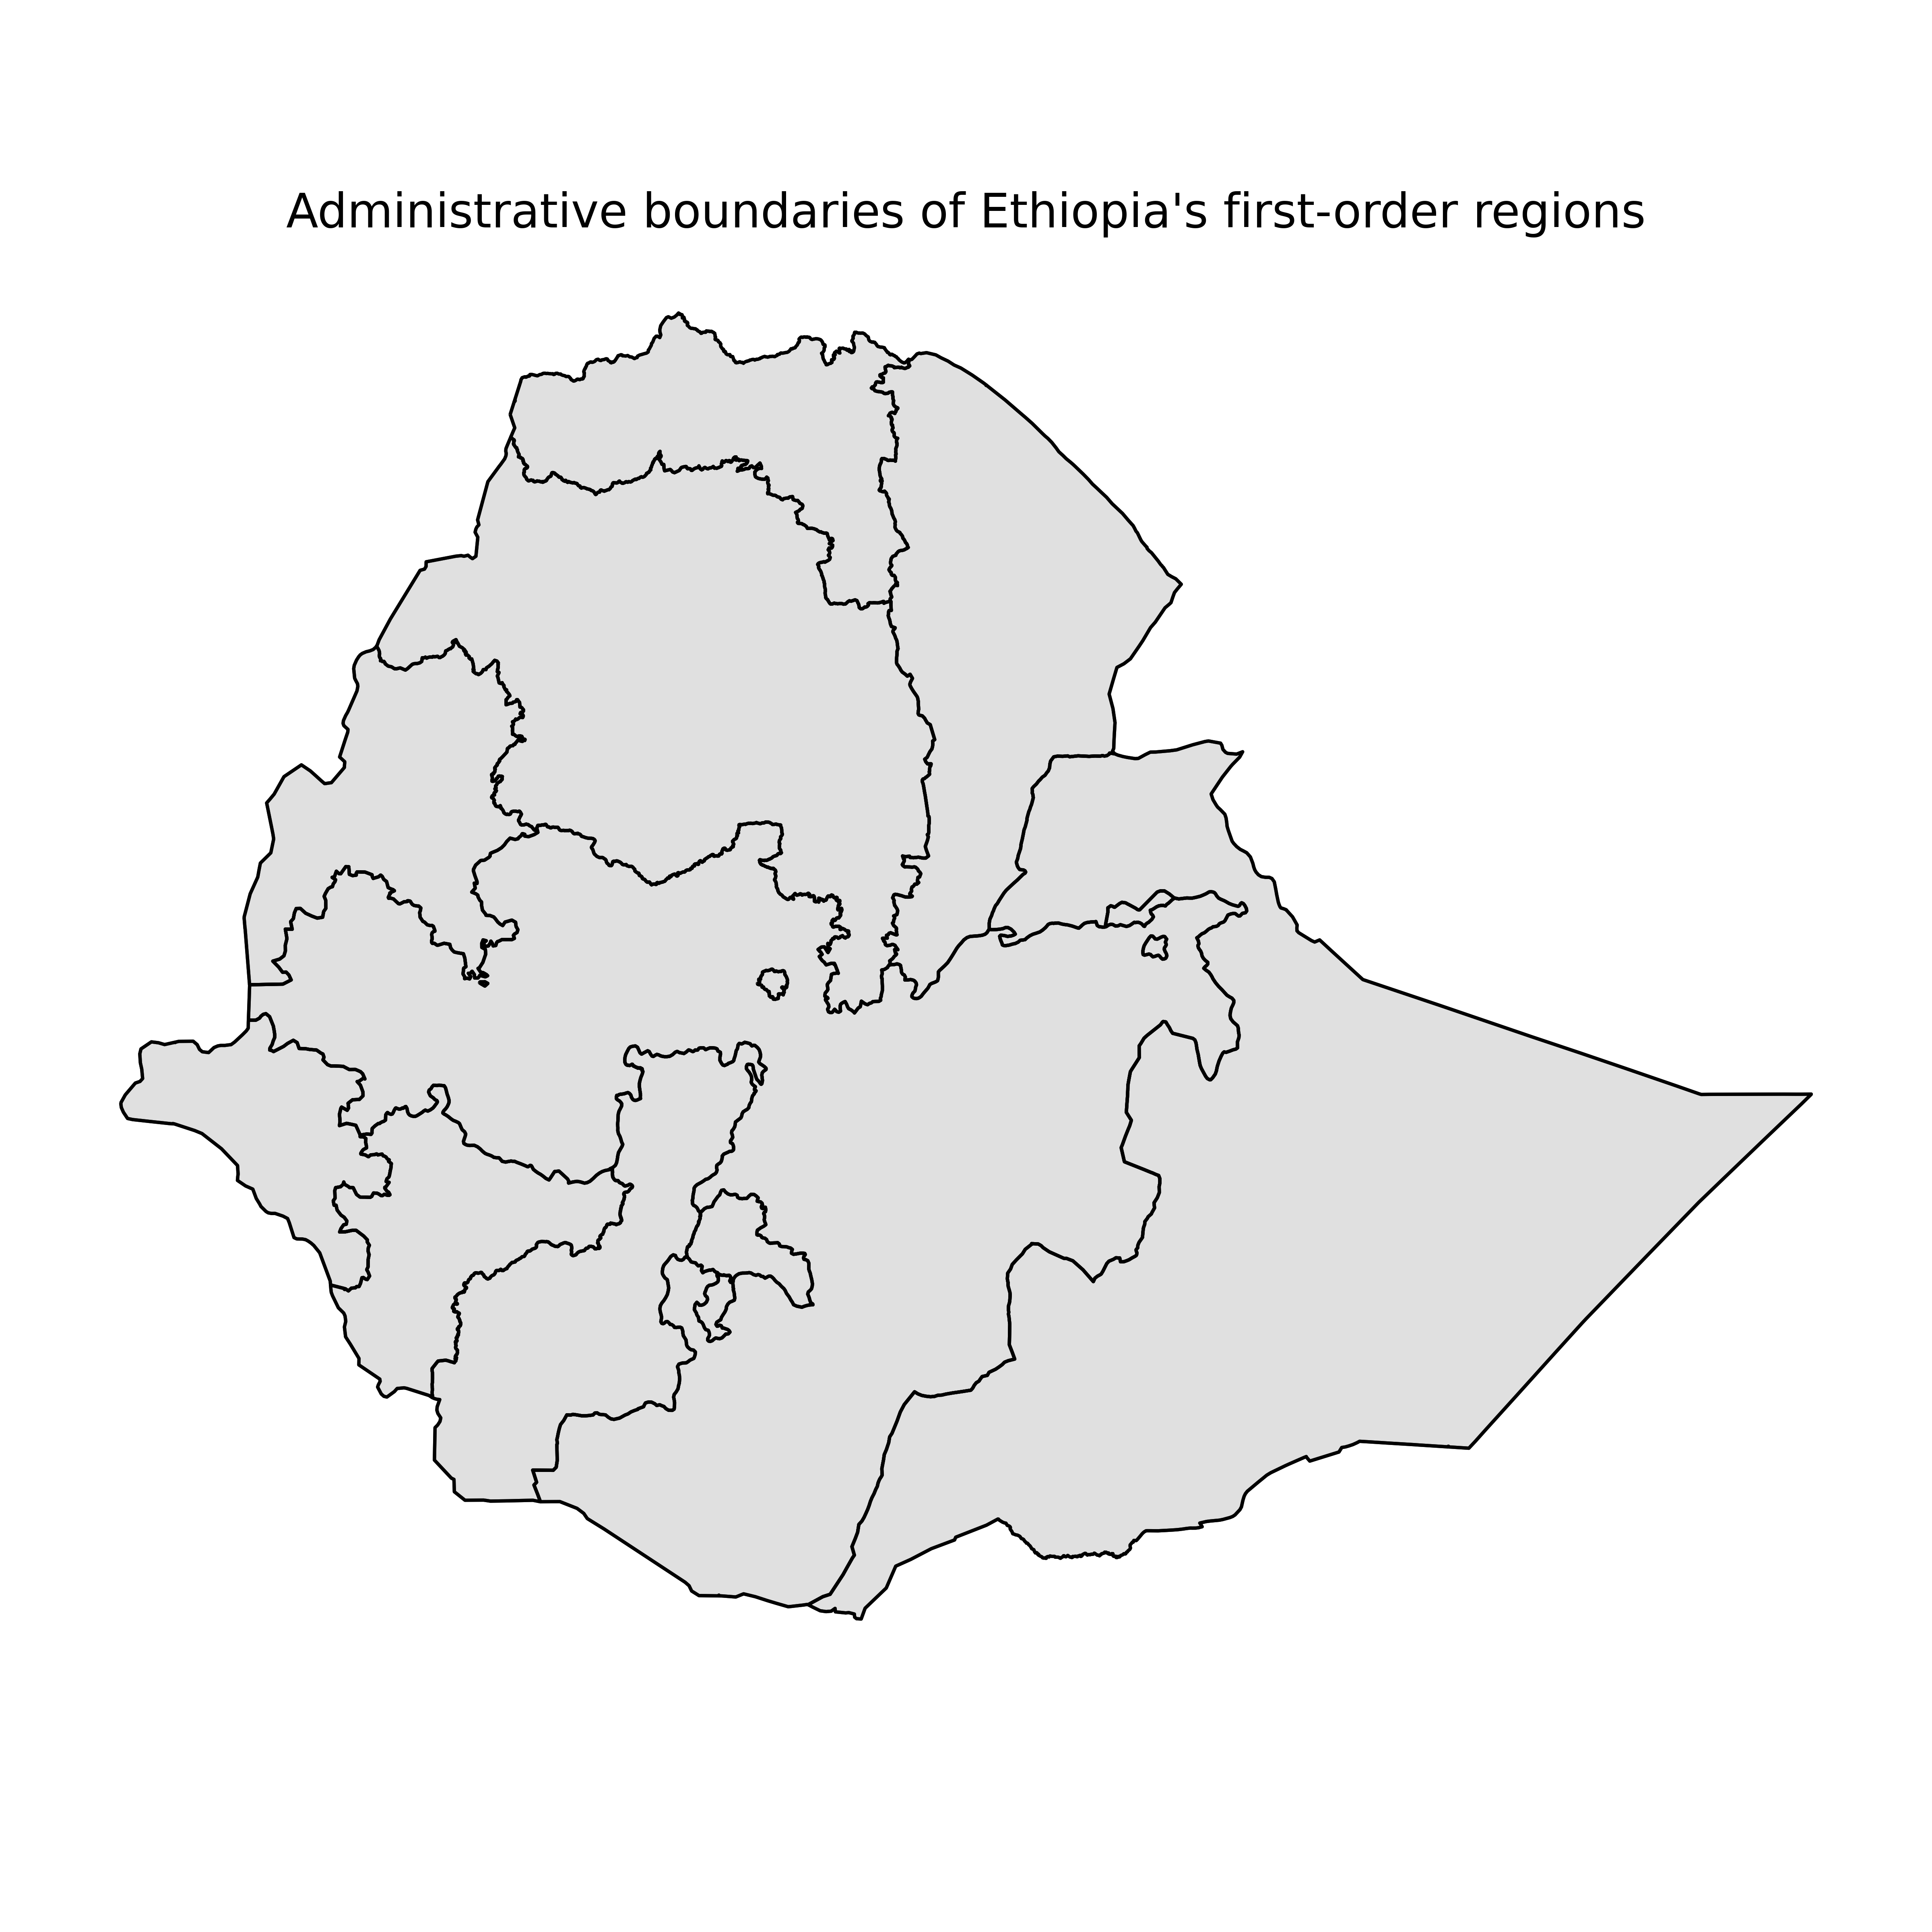
\includegraphics[width=0.7\textwidth]{outputs/figures/admin/ethiopia_admin_map.png}
	\caption{Administrative boundaries of Ethiopia's first-order regions. The map displays the 13 regional units used in the analysis, highlighting the evolving and fragmented nature of administrative boundaries over the study period.}
	\label{fig:admin_map}
\end{figure}
% --- End Figure 5 ---

\section{Identification Challenges in Small-N Panel Settings}

In empirical analyses of political favoritism using nighttime lights (NTL) data, identification is particularly challenging in settings with a small number of regions, limited exogenous variation in treatment, and high outcome concentration. This section outlines three core challenges that jointly limit inference in such panel data contexts.

\subsection{Omitted Variable Bias (without time fixed effects)}

When time fixed effects are omitted from panel regressions, estimates of leader-region favoritism are vulnerable to omitted variable bias. In the Ethiopian context, national economic shocks—such as booms or downturns—often coincide with leadership transitions. Without controlling for year effects, the estimated association between a leader’s birth region and regional luminosity may simply reflect these broader national trends, rather than any causal effect of political favoritism. Empirically, baseline models that exclude time fixed effects tend to produce inflated and statistically significant coefficients, but placebo tests and diagnostic plots reveal that these results are largely driven by common shocks rather than genuine treatment effects.

\subsection{Limited Identifying Variation (with time fixed effects)}

Including time fixed effects absorbs national shocks and common trends, but in small-N settings with few treated units and limited within-region, within-year variation, this approach introduces a new problem: limited identifying variation. When the timing of leader transitions is highly collinear with year effects, the model cannot reliably distinguish leader-region effects from national shocks. In the Ethiopian panel, the inclusion of time fixed effects sharply attenuates the estimated coefficients and increases standard errors, indicating that the available variation is insufficient for robust identification. The empirical p-values from placebo tests further confirm that observed effects are not distinguishable from random assignment.

\subsection{Low Statistical Power (small number of treated units)}

A third challenge is low statistical power, which arises from the small number of regions and limited number of leadership transitions. With only a handful of treated units and sparse treatment events, the effective sample size for identifying leader-region effects is severely constrained. This results in wide confidence intervals and imprecise estimates, particularly in event-study analyses and placebo simulations. The inability to detect dynamic effects or distinguish real from placebo results is a direct consequence of this low power, as demonstrated by the high empirical p-values and the overlap between observed and placebo distributions.

\paragraph{Synthesis}

Taken together, these challenges—omitted variable bias, limited identifying variation, and low statistical power—jointly undermine the credibility of causal inference in small-N panel settings. In the Ethiopian case, and in similar contexts, the combination of these factors means that apparent evidence for political favoritism is not empirically distinguishable from noise. Robust identification requires richer data, more exogenous variation, and careful diagnostic testing to avoid spurious findings.

\section{Literature Review}
This study sits at the intersection of three literatures.

First, a substantial literature uses satellite luminosity to measure economic activity. Early work established that light emissions track national and regional output surprisingly well in settings with limited conventional statistics \citep{Chen2011,Henderson2012}. More recent contributions show that the strength of this relationship varies with population density, sectoral composition, and spatial scale, which makes local interpretation more difficult than national validation exercises might suggest \citep{Bluhm2022,Gibson2021}. Work on harmonized long-run products has also improved the temporal comparability of DMSP-OLS and VIIRS series, but it has not eliminated measurement challenges \citep{Li2023,Gibson2024}.

Second, the paper relates to research on regional and ethnic favoritism. \citet{Hodler2014} show that political leaders' birth regions tend to receive higher nighttime light intensity in a broad cross-country sample. Subsequent work has refined that perspective by emphasizing the interaction between political favoritism, local ethnic demography, and institutions \citep{BeiserMcGrath2021}. Recent studies also continue to find geographically targeted favoritism in other settings, including public investment and local clientelism \citep{Onana2024,Cruzatti2024}. The implication is not that favoritism is universal, but that claims about it should be tested against within-unit changes rather than cross-sectional differences.




Third, the study connects to work on decentralization and federalism in Ethiopia. Existing scholarship highlights the tension between formal regional autonomy and persistent vertical control, including constraints on local fiscal autonomy and uneven developmental capacity \citep{Faguet2021,Wubneh2017}. Those institutional features make Ethiopia a theoretically important case for studying regional inequality, but they also heighten the need for careful empirical design. If regional trajectories differ for structural reasons unrelated to political leadership, pooled cross-sectional comparisons can easily be mistaken for favoritism.

\subsection*{Political Economy of Ethiopian Federalism}
The spatial distribution of rents in Ethiopia is deeply shaped by the country’s federal architecture and the political strategies of its ruling coalitions. Under the Ethiopian People’s Revolutionary Democratic Front (EPRDF), federalism was formally enshrined, but real power remained highly centralized. The EPRDF’s dominance over regional governments meant that resource allocation, investment, and development projects were often coordinated from the center, with regional administrations acting as agents rather than autonomous principals. This centralization is theorized to produce a spatial distribution of rents that is less responsive to local political dynamics and more reflective of national priorities and coalition management. In contrast, the current administration has presided over a period of greater regional contestation and, in some cases, increased regional autonomy. According to \citet{Faguet2021}, such shifts can alter the expected pattern of rent distribution: as regional governments gain more effective autonomy, the allocation of resources may become more sensitive to local political competition, ethnic demography, and the bargaining power of regional elites. This theoretical perspective suggests that the empirical analysis of favoritism in Ethiopia must account for changes in the structure of federalism and the evolving balance of power between center and regions.

Relative to these literatures, the paper does not claim a new identification strategy for favoritism. Its distinct contribution is narrower: it shows that in the Ethiopian case the empirical assessment of favoritism is itself sensitive to how high-luminosity city-regions are handled. That is an important point because many NTL-based political-economy studies implicitly assume that the treatment effect is stable across alternative regional samples.

\section{Methodology}
\subsection{Data}
\subsubsection{Nighttime light data}
The repository contains a harmonized annual NTL series built from DMSP-OLS and VIIRS raster products. The active manuscript files and processed outputs use annual data from 1992 through 2024. The underlying scripts reference the pixel-scale corrected nighttime light product of \citet{Li2023} and annual VIIRS composites derived by \citet{Elvidge2021}. Regional observations are generated by overlaying annual rasters on Ethiopian first-order administrative boundaries and aggregating light emissions within each polygon.

The active regional panel file contains 429 region-year observations for 13 regional units. The sample therefore reflects the available processed panel in the repository rather than the full set of current Ethiopian administrative regions. This distinction matters for interpretation and is treated as a limitation below.
% --- Begin Figure 5: Admin Map ---
\begin{figure}[ht]
	\centering
	% Replace the following line with the actual path to your admin map graphic
	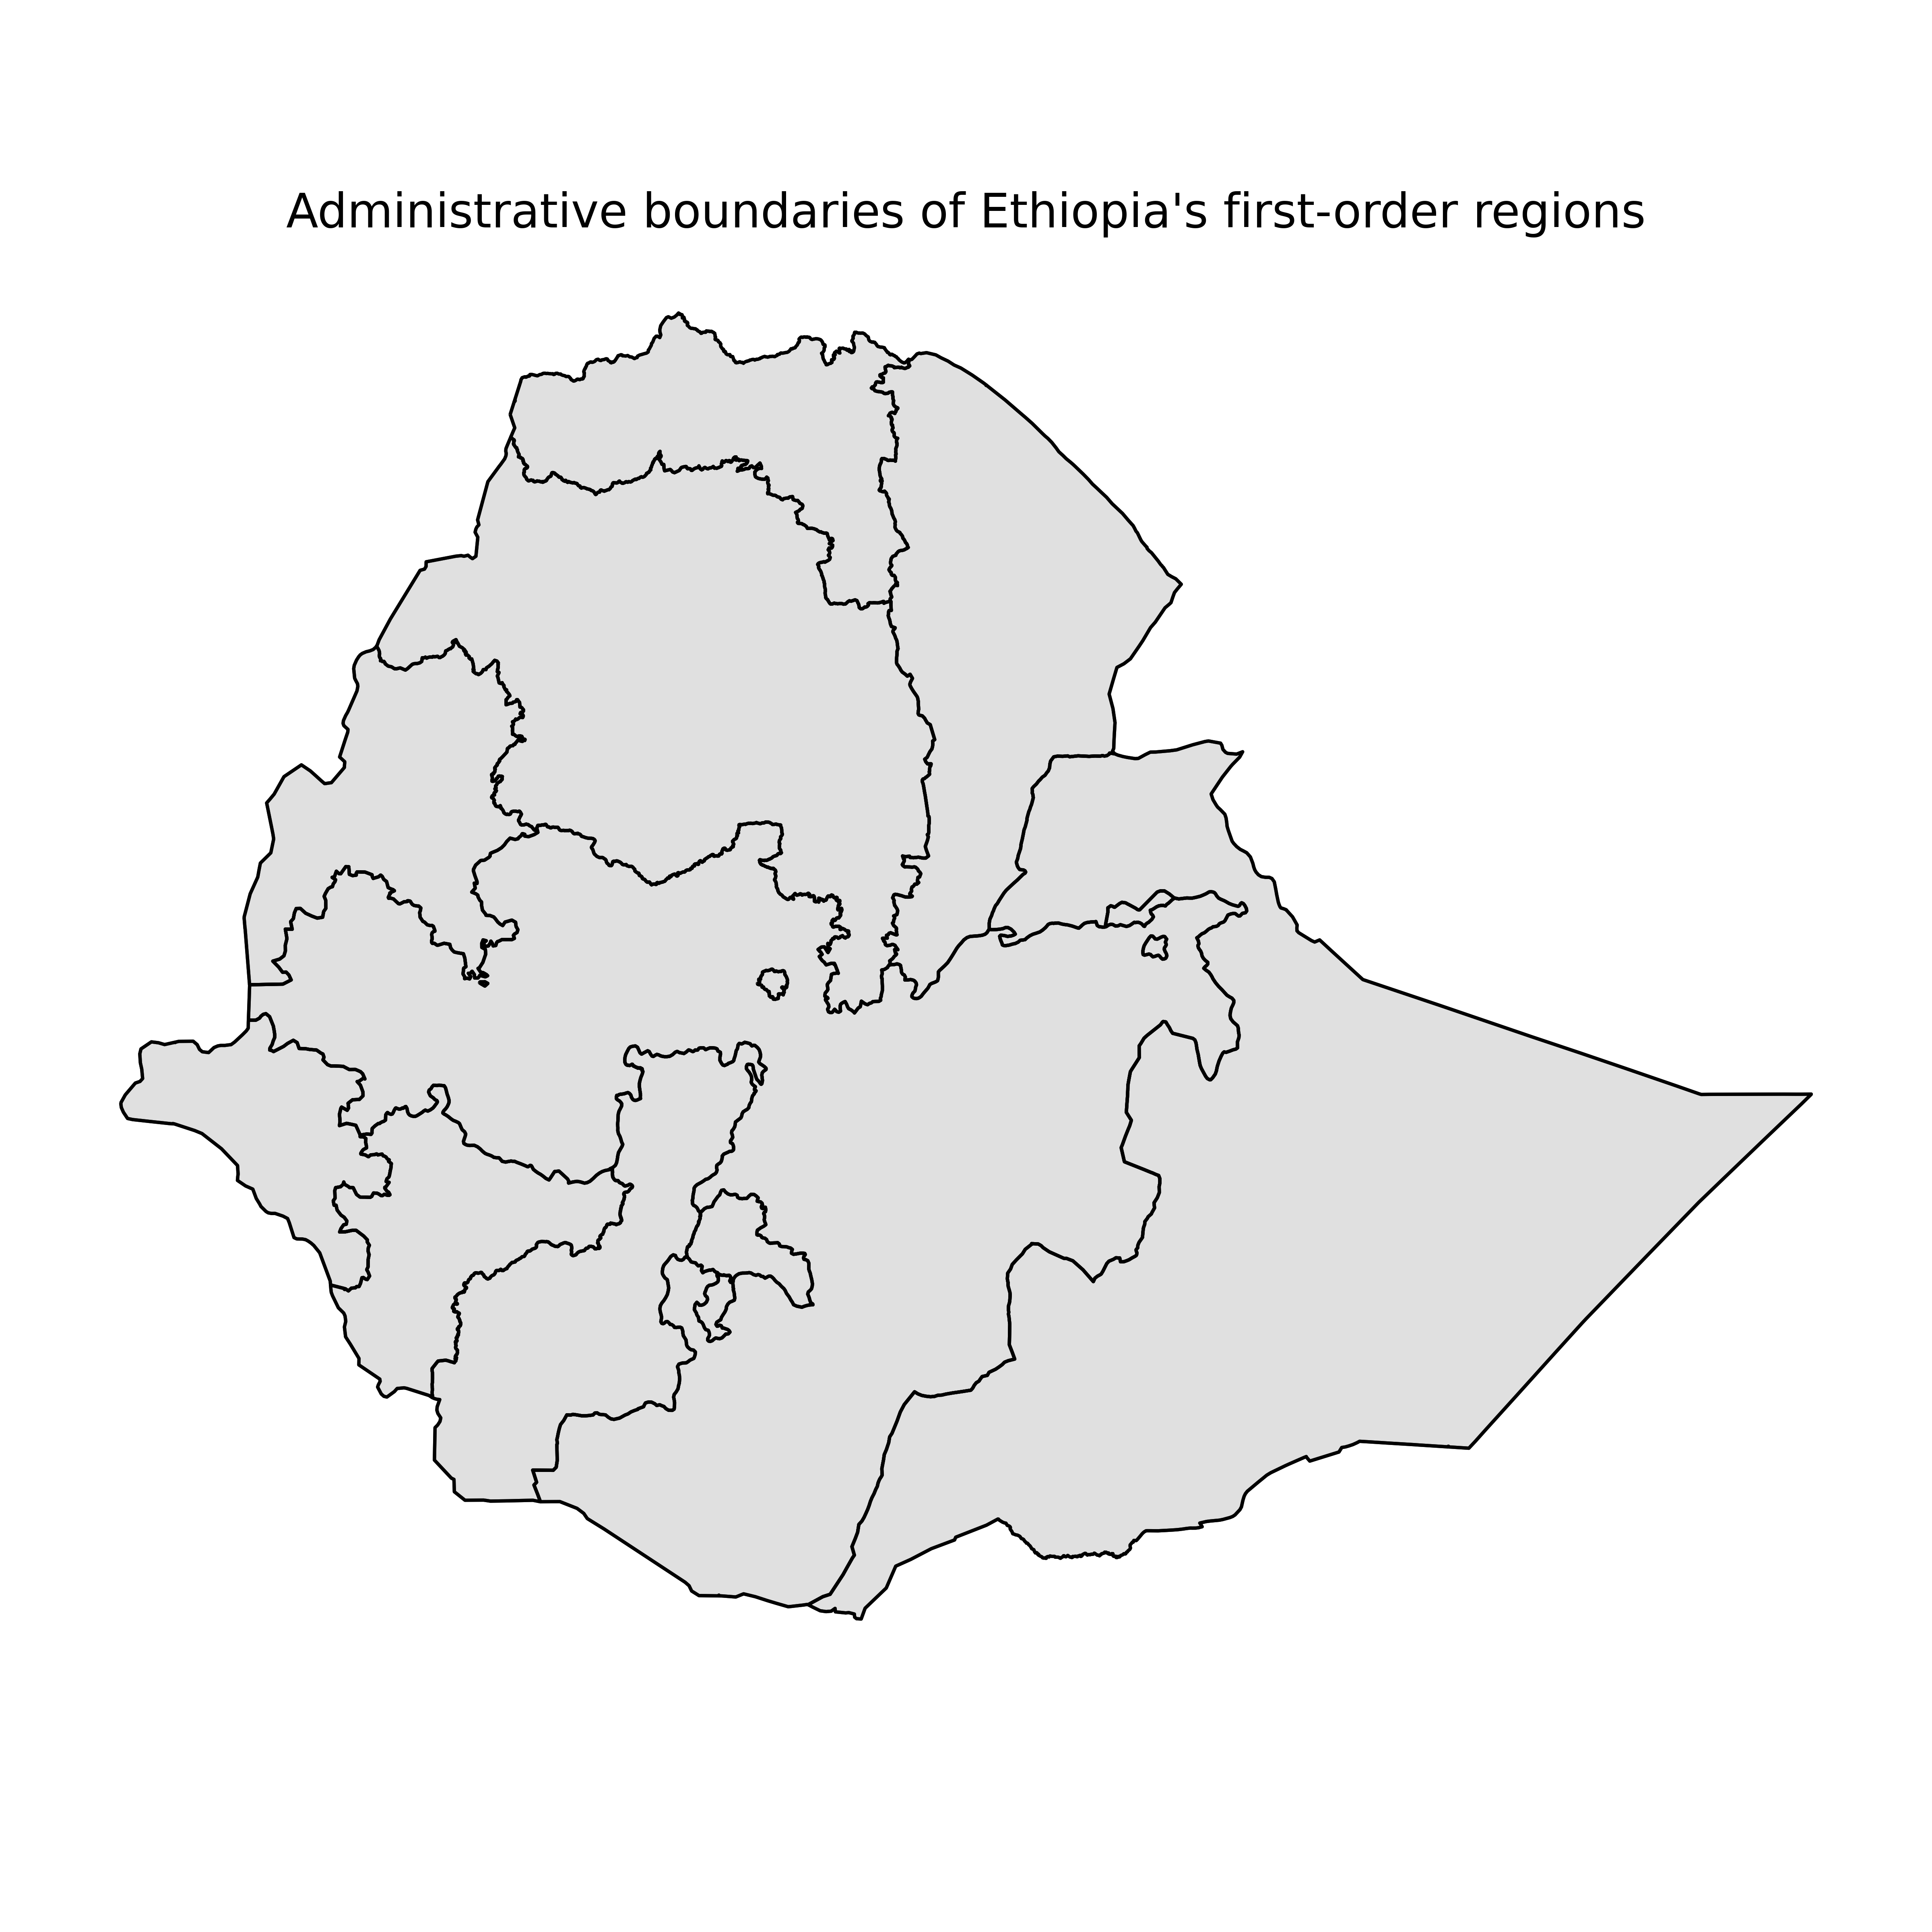
\includegraphics[width=0.7\textwidth]{outputs/figures/admin/ethiopia_admin_map.png}
	\caption{Administrative boundaries of Ethiopia's first-order regions. The map displays the 13 regional units used in the analysis, highlighting the evolving and fragmented nature of administrative boundaries over the study period.}
	\label{fig:admin_map}
\end{figure}
% --- End Figure 5 ---

\section{Identification Challenges in Small-N Panel Settings}

In empirical analyses of political favoritism using nighttime lights (NTL) data, identification is particularly challenging in settings with a small number of regions, limited exogenous variation in treatment, and high outcome concentration. This section outlines three core challenges that jointly limit inference in such panel data contexts.

\subsection{Omitted Variable Bias (without time fixed effects)}

When time fixed effects are omitted from panel regressions, estimates of leader-region favoritism are vulnerable to omitted variable bias. In the Ethiopian context, national economic shocks—such as booms or downturns—often coincide with leadership transitions. Without controlling for year effects, the estimated association between a leader’s birth region and regional luminosity may simply reflect these broader national trends, rather than any causal effect of political favoritism. Empirically, baseline models that exclude time fixed effects tend to produce inflated and statistically significant coefficients, but placebo tests and diagnostic plots reveal that these results are largely driven by common shocks rather than genuine treatment effects.

\subsection{Limited Identifying Variation (with time fixed effects)}

Including time fixed effects absorbs national shocks and common trends, but in small-N settings with few treated units and limited within-region, within-year variation, this approach introduces a new problem: limited identifying variation. When the timing of leader transitions is highly collinear with year effects, the model cannot reliably distinguish leader-region effects from national shocks. In the Ethiopian panel, the inclusion of time fixed effects sharply attenuates the estimated coefficients and increases standard errors, indicating that the available variation is insufficient for robust identification. The empirical p-values from placebo tests further confirm that observed effects are not distinguishable from random assignment.

\subsection{Low Statistical Power (small number of treated units)}

A third challenge is low statistical power, which arises from the small number of regions and limited number of leadership transitions. With only a handful of treated units and sparse treatment events, the effective sample size for identifying leader-region effects is severely constrained. This results in wide confidence intervals and imprecise estimates, particularly in event-study analyses and placebo simulations. The inability to detect dynamic effects or distinguish real from placebo results is a direct consequence of this low power, as demonstrated by the high empirical p-values and the overlap between observed and placebo distributions.

\paragraph{Synthesis}

Taken together, these challenges—omitted variable bias, limited identifying variation, and low statistical power—jointly undermine the credibility of causal inference in small-N panel settings. In the Ethiopian case, and in similar contexts, the combination of these factors means that apparent evidence for political favoritism is not empirically distinguishable from noise. Robust identification requires richer data, more exogenous variation, and careful diagnostic testing to avoid spurious findings.

\section{Literature Review}
This study sits at the intersection of three literatures.

First, a substantial literature uses satellite luminosity to measure economic activity. Early work established that light emissions track national and regional output surprisingly well in settings with limited conventional statistics \citep{Chen2011,Henderson2012}. More recent contributions show that the strength of this relationship varies with population density, sectoral composition, and spatial scale, which makes local interpretation more difficult than national validation exercises might suggest \citep{Bluhm2022,Gibson2021}. Work on harmonized long-run products has also improved the temporal comparability of DMSP-OLS and VIIRS series, but it has not eliminated measurement challenges \citep{Li2023,Gibson2024}.

Second, the paper relates to research on regional and ethnic favoritism. \citet{Hodler2014} show that political leaders' birth regions tend to receive higher nighttime light intensity in a broad cross-country sample. Subsequent work has refined that perspective by emphasizing the interaction between political favoritism, local ethnic demography, and institutions \citep{BeiserMcGrath2021}. Recent studies also continue to find geographically targeted favoritism in other settings, including public investment and local clientelism \citep{Onana2024,Cruzatti2024}. The implication is not that favoritism is universal, but that claims about it should be tested against within-unit changes rather than cross-sectional differences.




Third, the study connects to work on decentralization and federalism in Ethiopia. Existing scholarship highlights the tension between formal regional autonomy and persistent vertical control, including constraints on local fiscal autonomy and uneven developmental capacity \citep{Faguet2021,Wubneh2017}. Those institutional features make Ethiopia a theoretically important case for studying regional inequality, but they also heighten the need for careful empirical design. If regional trajectories differ for structural reasons unrelated to political leadership, pooled cross-sectional comparisons can easily be mistaken for favoritism.

\subsection*{Political Economy of Ethiopian Federalism}
The spatial distribution of rents in Ethiopia is deeply shaped by the country’s federal architecture and the political strategies of its ruling coalitions. Under the Ethiopian People’s Revolutionary Democratic Front (EPRDF), federalism was formally enshrined, but real power remained highly centralized. The EPRDF’s dominance over regional governments meant that resource allocation, investment, and development projects were often coordinated from the center, with regional administrations acting as agents rather than autonomous principals. This centralization is theorized to produce a spatial distribution of rents that is less responsive to local political dynamics and more reflective of national priorities and coalition management. In contrast, the current administration has presided over a period of greater regional contestation and, in some cases, increased regional autonomy. According to \citet{Faguet2021}, such shifts can alter the expected pattern of rent distribution: as regional governments gain more effective autonomy, the allocation of resources may become more sensitive to local political competition, ethnic demography, and the bargaining power of regional elites. This theoretical perspective suggests that the empirical analysis of favoritism in Ethiopia must account for changes in the structure of federalism and the evolving balance of power between center and regions.

Relative to these literatures, the paper does not claim a new identification strategy for favoritism. Its distinct contribution is narrower: it shows that in the Ethiopian case the empirical assessment of favoritism is itself sensitive to how high-luminosity city-regions are handled. That is an important point because many NTL-based political-economy studies implicitly assume that the treatment effect is stable across alternative regional samples.

\section{Methodology}
\subsection{Data}
\subsubsection{Nighttime light data}
The repository contains a harmonized annual NTL series built from DMSP-OLS and VIIRS raster products. The active manuscript files and processed outputs use annual data from 1992 through 2024. The underlying scripts reference the pixel-scale corrected nighttime light product of \citet{Li2023} and annual VIIRS composites derived by \citet{Elvidge2021}. Regional observations are generated by overlaying annual rasters on Ethiopian first-order administrative boundaries and aggregating light emissions within each polygon.

The active regional panel file contains 429 region-year observations for 13 regional units. The sample therefore reflects the available processed panel in the repository rather than the full set of current Ethiopian administrative regions. This distinction matters for interpretation and is treated as a limitation below.
% --- Begin Figure 5: Admin Map ---
\begin{figure}[ht]
	\centering
	% Replace the following line with the actual path to your admin map graphic
	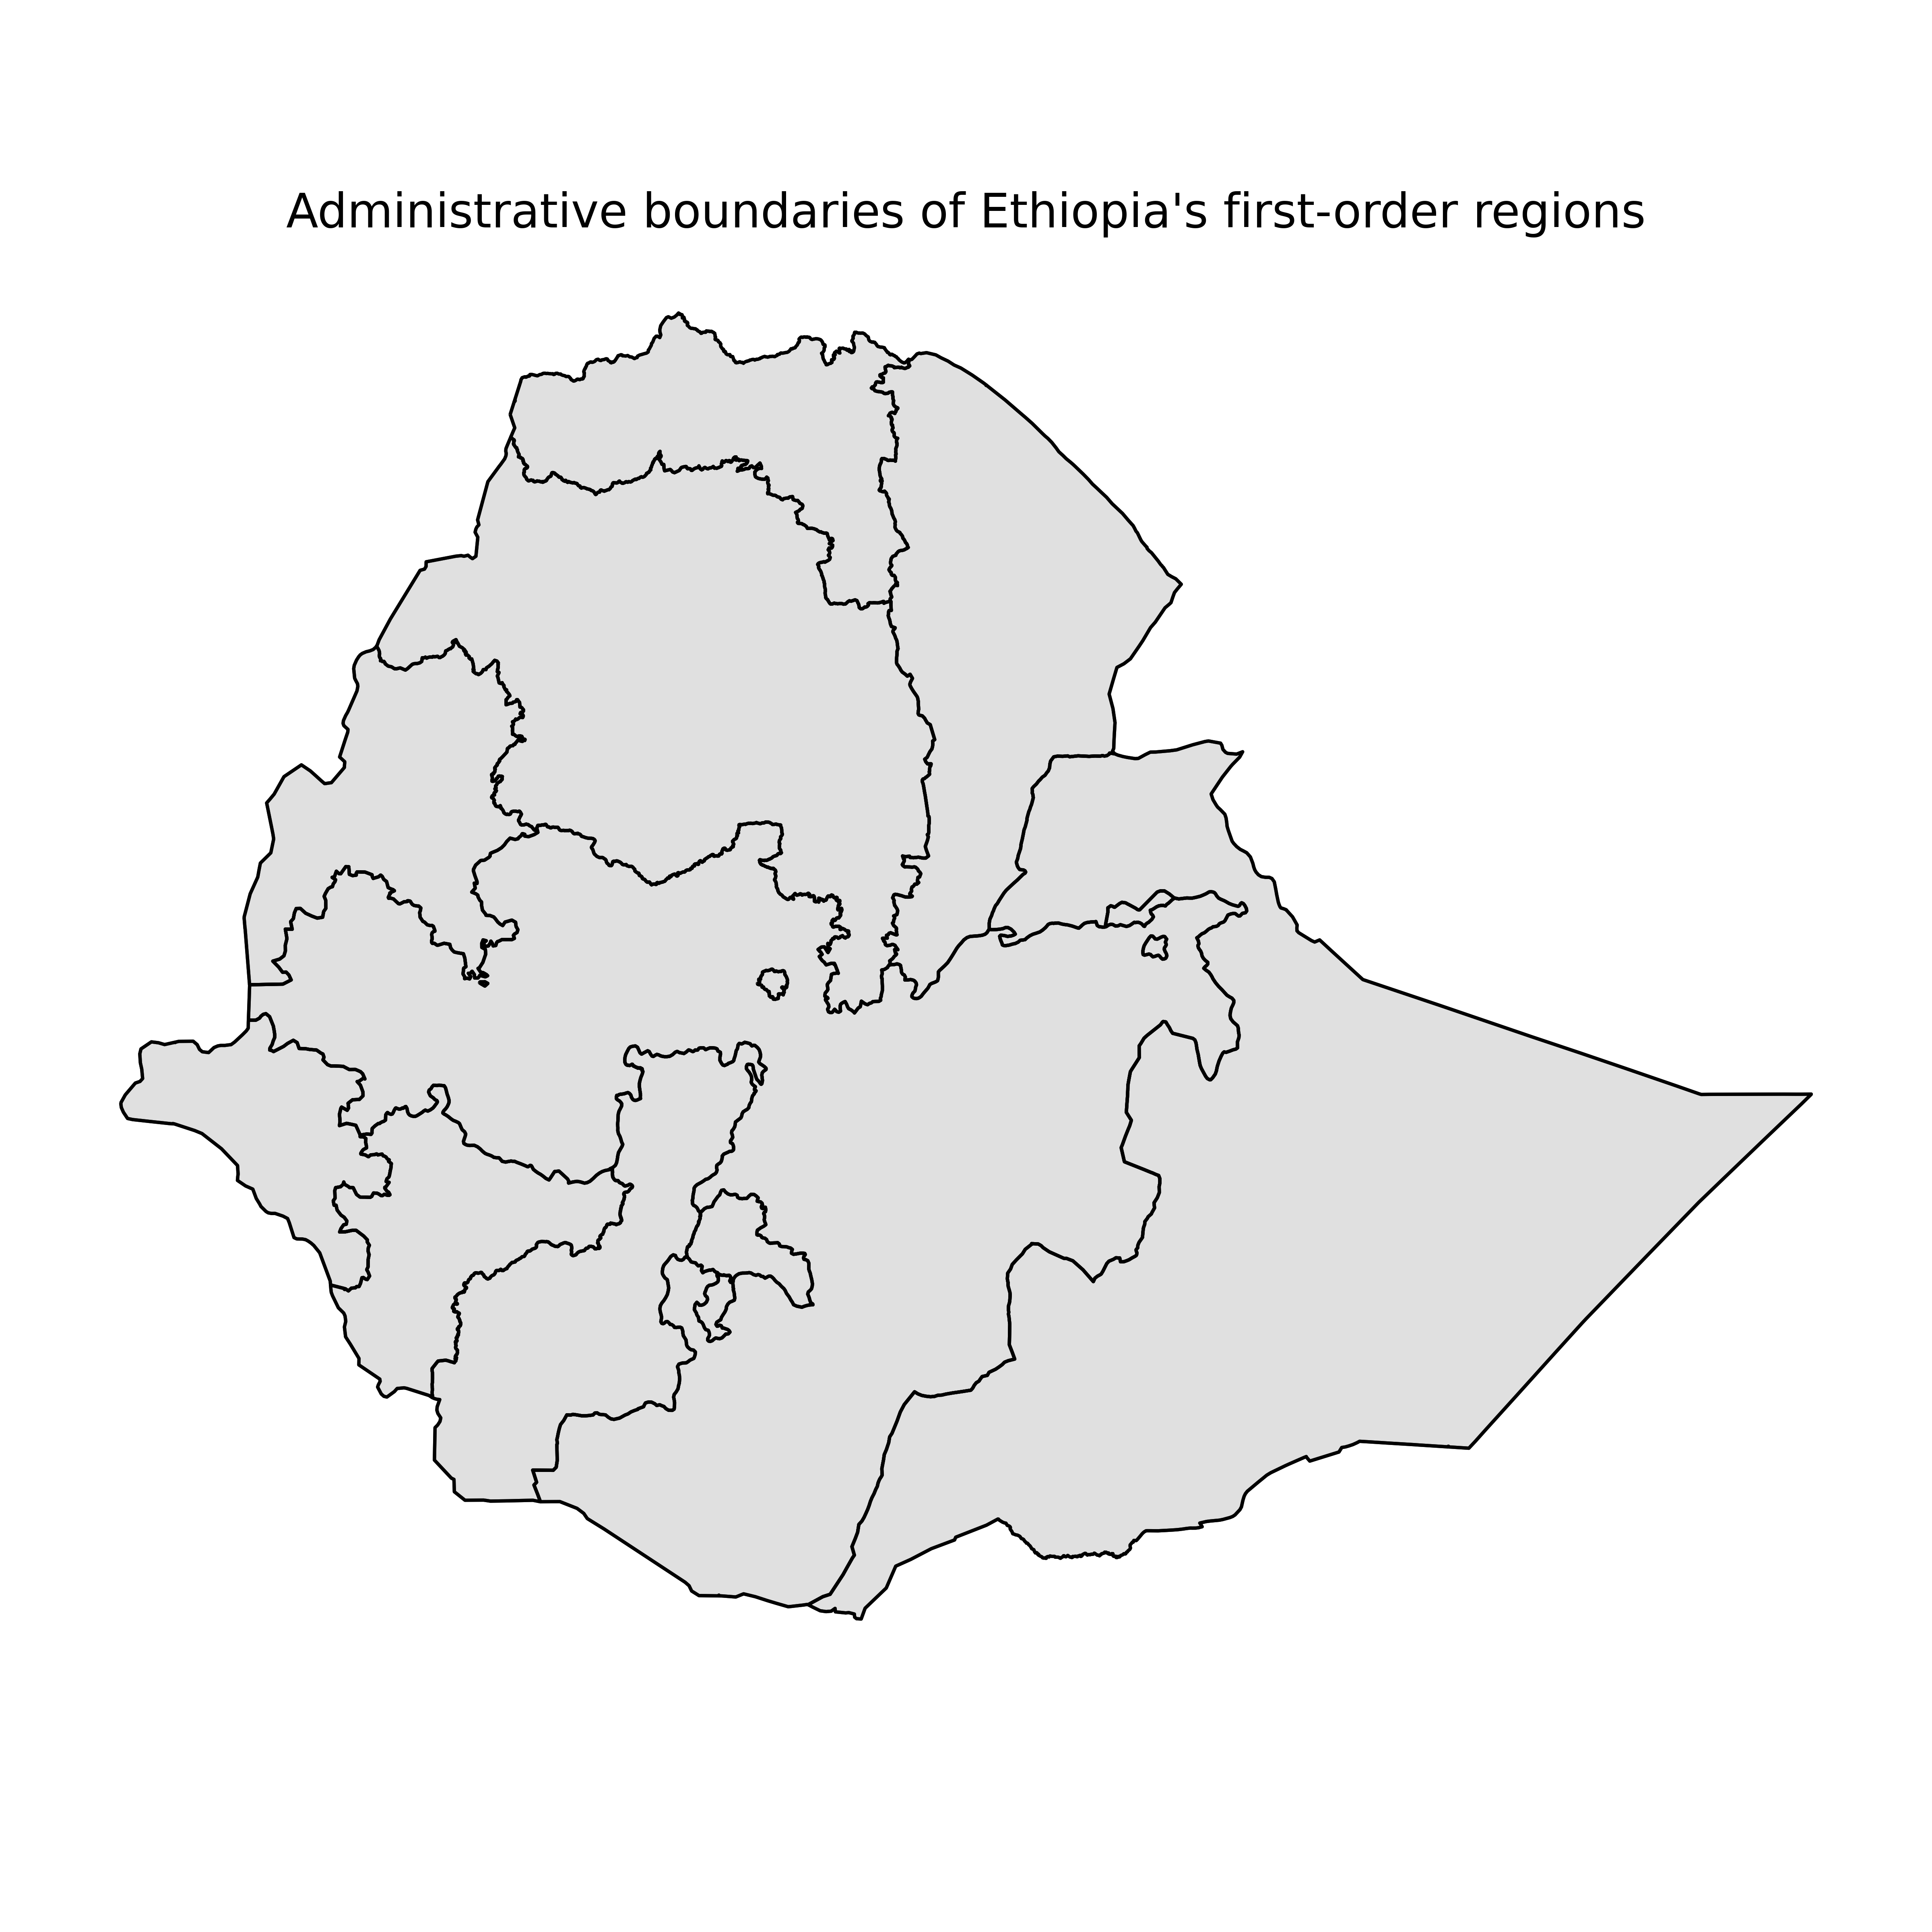
\includegraphics[width=0.7\textwidth]{outputs/figures/admin/ethiopia_admin_map.png}
	\caption{Administrative boundaries of Ethiopia's first-order regions. The map displays the 13 regional units used in the analysis, highlighting the evolving and fragmented nature of administrative boundaries over the study period.}
	\label{fig:admin_map}
\end{figure}
% --- End Figure 5 ---

\section{Identification Challenges in Small-N Panel Settings}

In empirical analyses of political favoritism using nighttime lights (NTL) data, identification is particularly challenging in settings with a small number of regions, limited exogenous variation in treatment, and high outcome concentration. This section outlines three core challenges that jointly limit inference in such panel data contexts.

\subsection{Omitted Variable Bias (without time fixed effects)}

When time fixed effects are omitted from panel regressions, estimates of leader-region favoritism are vulnerable to omitted variable bias. In the Ethiopian context, national economic shocks—such as booms or downturns—often coincide with leadership transitions. Without controlling for year effects, the estimated association between a leader’s birth region and regional luminosity may simply reflect these broader national trends, rather than any causal effect of political favoritism. Empirically, baseline models that exclude time fixed effects tend to produce inflated and statistically significant coefficients, but placebo tests and diagnostic plots reveal that these results are largely driven by common shocks rather than genuine treatment effects.

\subsection{Limited Identifying Variation (with time fixed effects)}

Including time fixed effects absorbs national shocks and common trends, but in small-N settings with few treated units and limited within-region, within-year variation, this approach introduces a new problem: limited identifying variation. When the timing of leader transitions is highly collinear with year effects, the model cannot reliably distinguish leader-region effects from national shocks. In the Ethiopian panel, the inclusion of time fixed effects sharply attenuates the estimated coefficients and increases standard errors, indicating that the available variation is insufficient for robust identification. The empirical p-values from placebo tests further confirm that observed effects are not distinguishable from random assignment.

\subsection{Low Statistical Power (small number of treated units)}

A third challenge is low statistical power, which arises from the small number of regions and limited number of leadership transitions. With only a handful of treated units and sparse treatment events, the effective sample size for identifying leader-region effects is severely constrained. This results in wide confidence intervals and imprecise estimates, particularly in event-study analyses and placebo simulations. The inability to detect dynamic effects or distinguish real from placebo results is a direct consequence of this low power, as demonstrated by the high empirical p-values and the overlap between observed and placebo distributions.

\paragraph{Synthesis}

Taken together, these challenges—omitted variable bias, limited identifying variation, and low statistical power—jointly undermine the credibility of causal inference in small-N panel settings. In the Ethiopian case, and in similar contexts, the combination of these factors means that apparent evidence for political favoritism is not empirically distinguishable from noise. Robust identification requires richer data, more exogenous variation, and careful diagnostic testing to avoid spurious findings.

\section{Literature Review}
This study sits at the intersection of three literatures.

First, a substantial literature uses satellite luminosity to measure economic activity. Early work established that light emissions track national and regional output surprisingly well in settings with limited conventional statistics \citep{Chen2011,Henderson2012}. More recent contributions show that the strength of this relationship varies with population density, sectoral composition, and spatial scale, which makes local interpretation more difficult than national validation exercises might suggest \citep{Bluhm2022,Gibson2021}. Work on harmonized long-run products has also improved the temporal comparability of DMSP-OLS and VIIRS series, but it has not eliminated measurement challenges \citep{Li2023,Gibson2024}.

Second, the paper relates to research on regional and ethnic favoritism. \citet{Hodler2014} show that political leaders' birth regions tend to receive higher nighttime light intensity in a broad cross-country sample. Subsequent work has refined that perspective by emphasizing the interaction between political favoritism, local ethnic demography, and institutions \citep{BeiserMcGrath2021}. Recent studies also continue to find geographically targeted favoritism in other settings, including public investment and local clientelism \citep{Onana2024,Cruzatti2024}. The implication is not that favoritism is universal, but that claims about it should be tested against within-unit changes rather than cross-sectional differences.




Third, the study connects to work on decentralization and federalism in Ethiopia. Existing scholarship highlights the tension between formal regional autonomy and persistent vertical control, including constraints on local fiscal autonomy and uneven developmental capacity \citep{Faguet2021,Wubneh2017}. Those institutional features make Ethiopia a theoretically important case for studying regional inequality, but they also heighten the need for careful empirical design. If regional trajectories differ for structural reasons unrelated to political leadership, pooled cross-sectional comparisons can easily be mistaken for favoritism.

\subsection*{Political Economy of Ethiopian Federalism}
The spatial distribution of rents in Ethiopia is deeply shaped by the country’s federal architecture and the political strategies of its ruling coalitions. Under the Ethiopian People’s Revolutionary Democratic Front (EPRDF), federalism was formally enshrined, but real power remained highly centralized. The EPRDF’s dominance over regional governments meant that resource allocation, investment, and development projects were often coordinated from the center, with regional administrations acting as agents rather than autonomous principals. This centralization is theorized to produce a spatial distribution of rents that is less responsive to local political dynamics and more reflective of national priorities and coalition management. In contrast, the current administration has presided over a period of greater regional contestation and, in some cases, increased regional autonomy. According to \citet{Faguet2021}, such shifts can alter the expected pattern of rent distribution: as regional governments gain more effective autonomy, the allocation of resources may become more sensitive to local political competition, ethnic demography, and the bargaining power of regional elites. This theoretical perspective suggests that the empirical analysis of favoritism in Ethiopia must account for changes in the structure of federalism and the evolving balance of power between center and regions.

Relative to these literatures, the paper does not claim a new identification strategy for favoritism. Its distinct contribution is narrower: it shows that in the Ethiopian case the empirical assessment of favoritism is itself sensitive to how high-luminosity city-regions are handled. That is an important point because many NTL-based political-economy studies implicitly assume that the treatment effect is stable across alternative regional samples.

\section{Methodology}
\subsection{Data}
\subsubsection{Nighttime light data}
The repository contains a harmonized annual NTL series built from DMSP-OLS and VIIRS raster products. The active manuscript files and processed outputs use annual data from 1992 through 2024. The underlying scripts reference the pixel-scale corrected nighttime light product of \citet{Li2023} and annual VIIRS composites derived by \citet{Elvidge2021}. Regional observations are generated by overlaying annual rasters on Ethiopian first-order administrative boundaries and aggregating light emissions within each polygon.

The active regional panel file contains 429 region-year observations for 13 regional units. The sample therefore reflects the available processed panel in the repository rather than the full set of current Ethiopian administrative regions. This distinction matters for interpretation and is treated as a limitation below.
% --- Begin Figure 5: Admin Map ---
\begin{figure}[ht]
	\centering
	% Replace the following line with the actual path to your admin map graphic
	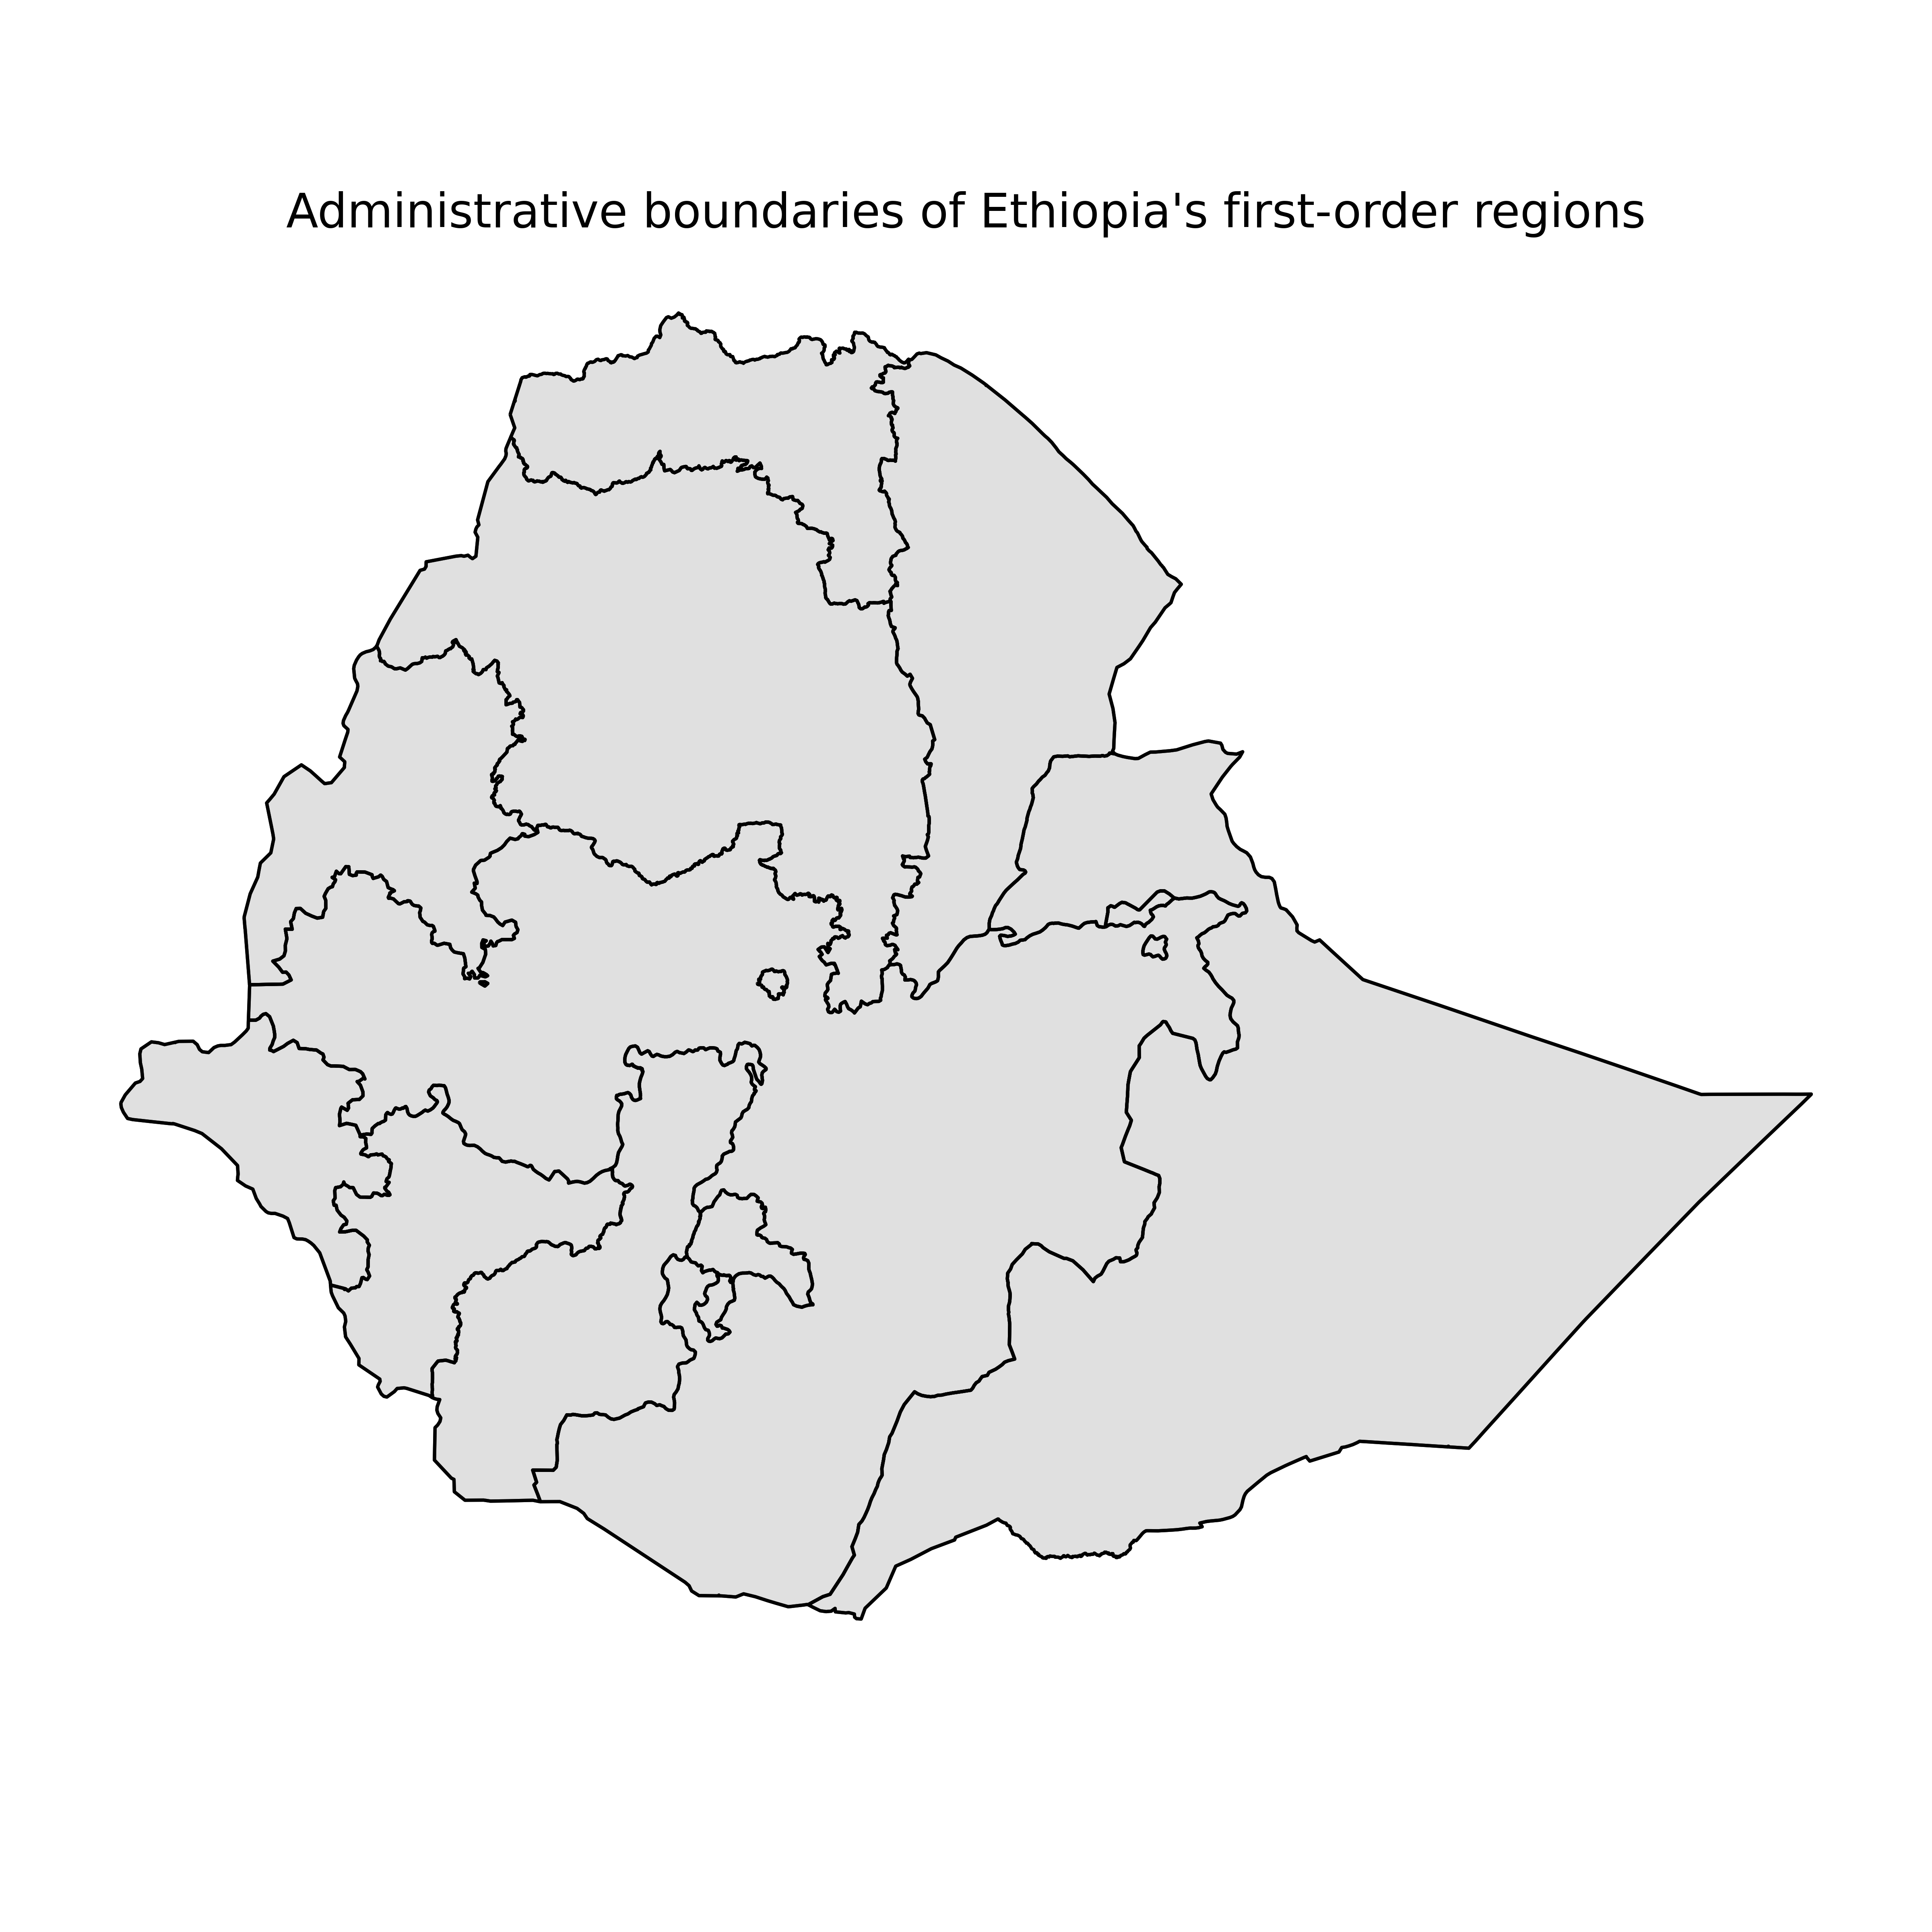
\includegraphics[width=0.7\textwidth]{outputs/figures/admin/ethiopia_admin_map.png}
	\caption{Administrative boundaries of Ethiopia's first-order regions. The map displays the 13 regional units used in the analysis, highlighting the evolving and fragmented nature of administrative boundaries over the study period.}
	\label{fig:admin_map}
\end{figure}
% --- End Figure 5 ---

\section{Identification Challenges in Small-N Panel Settings}

In empirical analyses of political favoritism using nighttime lights (NTL) data, identification is particularly challenging in settings with a small number of regions, limited exogenous variation in treatment, and high outcome concentration. This section outlines three core challenges that jointly limit inference in such panel data contexts.

\subsection{Omitted Variable Bias (without time fixed effects)}

When time fixed effects are omitted from panel regressions, estimates of leader-region favoritism are vulnerable to omitted variable bias. In the Ethiopian context, national economic shocks—such as booms or downturns—often coincide with leadership transitions. Without controlling for year effects, the estimated association between a leader’s birth region and regional luminosity may simply reflect these broader national trends, rather than any causal effect of political favoritism. Empirically, baseline models that exclude time fixed effects tend to produce inflated and statistically significant coefficients, but placebo tests and diagnostic plots reveal that these results are largely driven by common shocks rather than genuine treatment effects.

\subsection{Limited Identifying Variation (with time fixed effects)}

Including time fixed effects absorbs national shocks and common trends, but in small-N settings with few treated units and limited within-region, within-year variation, this approach introduces a new problem: limited identifying variation. When the timing of leader transitions is highly collinear with year effects, the model cannot reliably distinguish leader-region effects from national shocks. In the Ethiopian panel, the inclusion of time fixed effects sharply attenuates the estimated coefficients and increases standard errors, indicating that the available variation is insufficient for robust identification. The empirical p-values from placebo tests further confirm that observed effects are not distinguishable from random assignment.

\subsection{Low Statistical Power (small number of treated units)}

A third challenge is low statistical power, which arises from the small number of regions and limited number of leadership transitions. With only a handful of treated units and sparse treatment events, the effective sample size for identifying leader-region effects is severely constrained. This results in wide confidence intervals and imprecise estimates, particularly in event-study analyses and placebo simulations. The inability to detect dynamic effects or distinguish real from placebo results is a direct consequence of this low power, as demonstrated by the high empirical p-values and the overlap between observed and placebo distributions.

\paragraph{Synthesis}

Taken together, these challenges—omitted variable bias, limited identifying variation, and low statistical power—jointly undermine the credibility of causal inference in small-N panel settings. In the Ethiopian case, and in similar contexts, the combination of these factors means that apparent evidence for political favoritism is not empirically distinguishable from noise. Robust identification requires richer data, more exogenous variation, and careful diagnostic testing to avoid spurious findings.

\section{Literature Review}
This study sits at the intersection of three literatures.

First, a substantial literature uses satellite luminosity to measure economic activity. Early work established that light emissions track national and regional output surprisingly well in settings with limited conventional statistics \citep{Chen2011,Henderson2012}. More recent contributions show that the strength of this relationship varies with population density, sectoral composition, and spatial scale, which makes local interpretation more difficult than national validation exercises might suggest \citep{Bluhm2022,Gibson2021}. Work on harmonized long-run products has also improved the temporal comparability of DMSP-OLS and VIIRS series, but it has not eliminated measurement challenges \citep{Li2023,Gibson2024}.

Second, the paper relates to research on regional and ethnic favoritism. \citet{Hodler2014} show that political leaders' birth regions tend to receive higher nighttime light intensity in a broad cross-country sample. Subsequent work has refined that perspective by emphasizing the interaction between political favoritism, local ethnic demography, and institutions \citep{BeiserMcGrath2021}. Recent studies also continue to find geographically targeted favoritism in other settings, including public investment and local clientelism \citep{Onana2024,Cruzatti2024}. The implication is not that favoritism is universal, but that claims about it should be tested against within-unit changes rather than cross-sectional differences.




Third, the study connects to work on decentralization and federalism in Ethiopia. Existing scholarship highlights the tension between formal regional autonomy and persistent vertical control, including constraints on local fiscal autonomy and uneven developmental capacity \citep{Faguet2021,Wubneh2017}. Those institutional features make Ethiopia a theoretically important case for studying regional inequality, but they also heighten the need for careful empirical design. If regional trajectories differ for structural reasons unrelated to political leadership, pooled cross-sectional comparisons can easily be mistaken for favoritism.

\subsection*{Political Economy of Ethiopian Federalism}
The spatial distribution of rents in Ethiopia is deeply shaped by the country’s federal architecture and the political strategies of its ruling coalitions. Under the Ethiopian People’s Revolutionary Democratic Front (EPRDF), federalism was formally enshrined, but real power remained highly centralized. The EPRDF’s dominance over regional governments meant that resource allocation, investment, and development projects were often coordinated from the center, with regional administrations acting as agents rather than autonomous principals. This centralization is theorized to produce a spatial distribution of rents that is less responsive to local political dynamics and more reflective of national priorities and coalition management. In contrast, the current administration has presided over a period of greater regional contestation and, in some cases, increased regional autonomy. According to \citet{Faguet2021}, such shifts can alter the expected pattern of rent distribution: as regional governments gain more effective autonomy, the allocation of resources may become more sensitive to local political competition, ethnic demography, and the bargaining power of regional elites. This theoretical perspective suggests that the empirical analysis of favoritism in Ethiopia must account for changes in the structure of federalism and the evolving balance of power between center and regions.

Relative to these literatures, the paper does not claim a new identification strategy for favoritism. Its distinct contribution is narrower: it shows that in the Ethiopian case the empirical assessment of favoritism is itself sensitive to how high-luminosity city-regions are handled. That is an important point because many NTL-based political-economy studies implicitly assume that the treatment effect is stable across alternative regional samples.

\section{Methodology}
\subsection{Data}
\subsubsection{Nighttime light data}
The repository contains a harmonized annual NTL series built from DMSP-OLS and VIIRS raster products. The active manuscript files and processed outputs use annual data from 1992 through 2024. The underlying scripts reference the pixel-scale corrected nighttime light product of \citet{Li2023} and annual VIIRS composites derived by \citet{Elvidge2021}. Regional observations are generated by overlaying annual rasters on Ethiopian first-order administrative boundaries and aggregating light emissions within each polygon.

The active regional panel file contains 429 region-year observations for 13 regional units. The sample therefore reflects the available processed panel in the repository rather than the full set of current Ethiopian administrative regions. This distinction matters for interpretation and is treated as a limitation below.
% --- Begin Figure 5: Admin Map ---
\begin{figure}[ht]
	\centering
	% Replace the following line with the actual path to your admin map graphic
	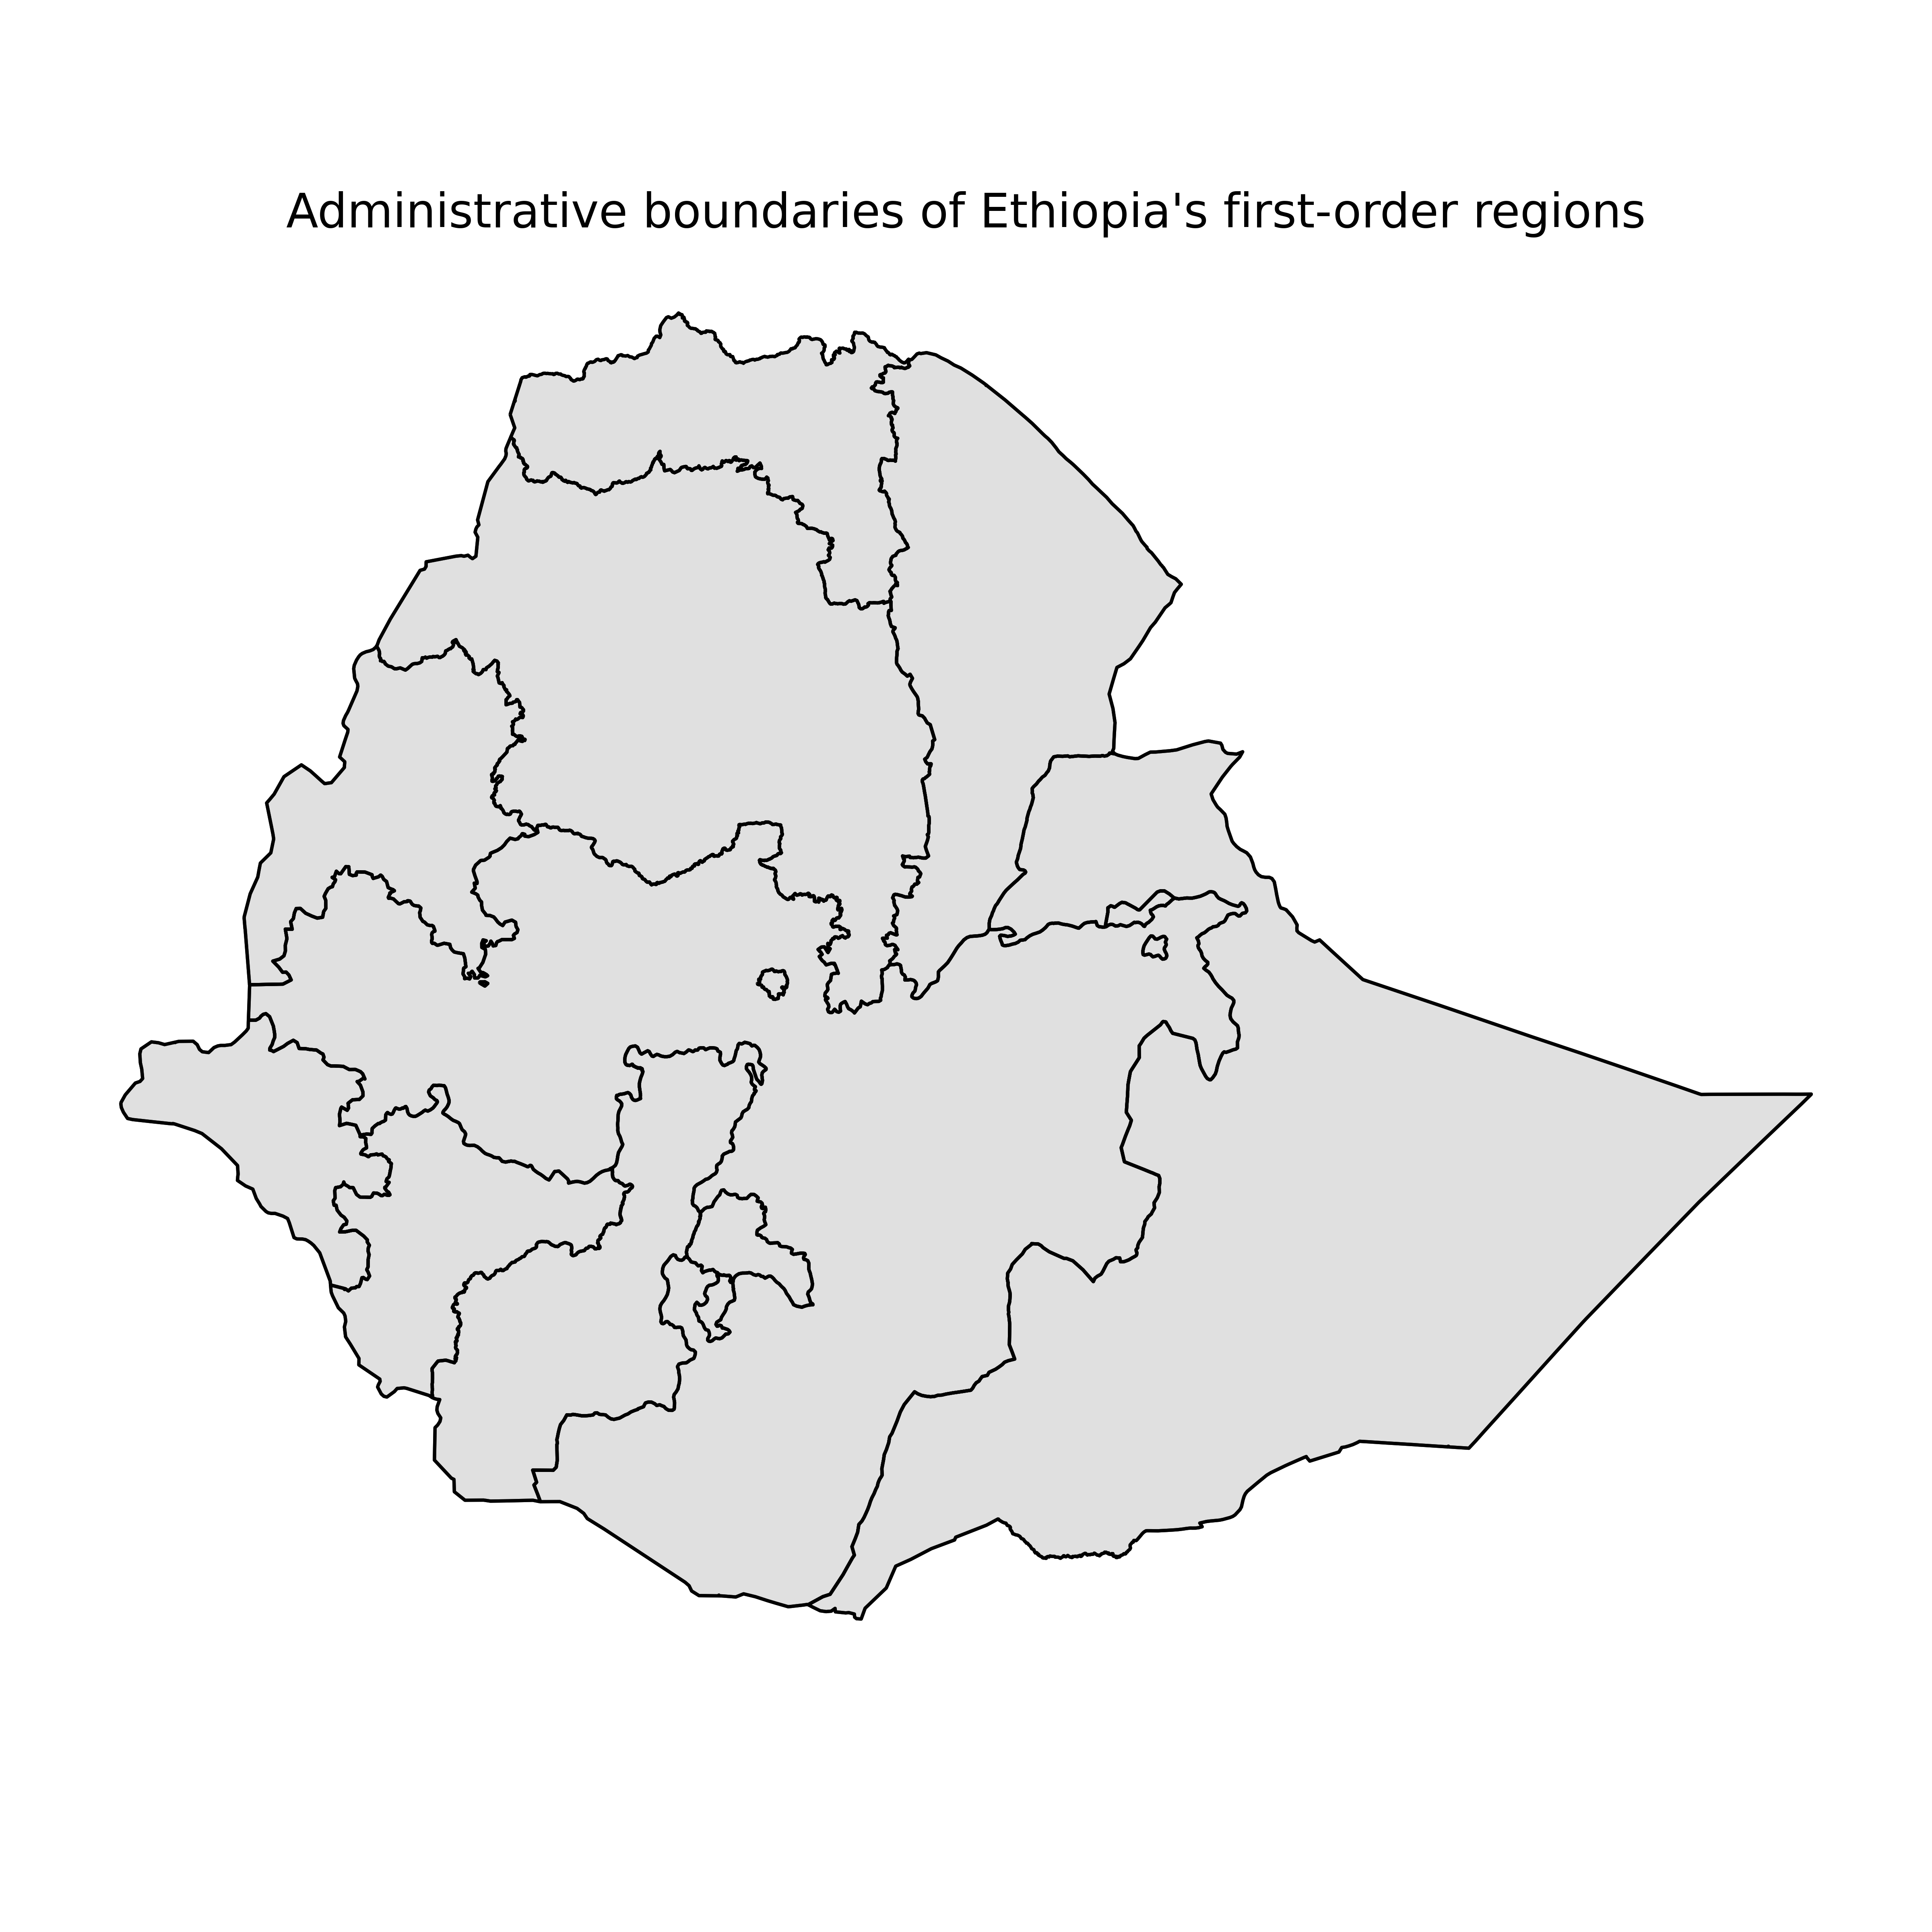
\includegraphics[width=0.7\textwidth]{outputs/figures/admin/ethiopia_admin_map.png}
	\caption{Administrative boundaries of Ethiopia's first-order regions. The map displays the 13 regional units used in the analysis, highlighting the evolving and fragmented nature of administrative boundaries over the study period.}
	\label{fig:admin_map}
\end{figure}
% --- End Figure 5 ---

\section{Identification Challenges in Small-N Panel Settings}

In empirical analyses of political favoritism using nighttime lights (NTL) data, identification is particularly challenging in settings with a small number of regions, limited exogenous variation in treatment, and high outcome concentration. This section outlines three core challenges that jointly limit inference in such panel data contexts.

\subsection{Omitted Variable Bias (without time fixed effects)}

When time fixed effects are omitted from panel regressions, estimates of leader-region favoritism are vulnerable to omitted variable bias. In the Ethiopian context, national economic shocks—such as booms or downturns—often coincide with leadership transitions. Without controlling for year effects, the estimated association between a leader’s birth region and regional luminosity may simply reflect these broader national trends, rather than any causal effect of political favoritism. Empirically, baseline models that exclude time fixed effects tend to produce inflated and statistically significant coefficients, but placebo tests and diagnostic plots reveal that these results are largely driven by common shocks rather than genuine treatment effects.

\subsection{Limited Identifying Variation (with time fixed effects)}

Including time fixed effects absorbs national shocks and common trends, but in small-N settings with few treated units and limited within-region, within-year variation, this approach introduces a new problem: limited identifying variation. When the timing of leader transitions is highly collinear with year effects, the model cannot reliably distinguish leader-region effects from national shocks. In the Ethiopian panel, the inclusion of time fixed effects sharply attenuates the estimated coefficients and increases standard errors, indicating that the available variation is insufficient for robust identification. The empirical p-values from placebo tests further confirm that observed effects are not distinguishable from random assignment.

\subsection{Low Statistical Power (small number of treated units)}

A third challenge is low statistical power, which arises from the small number of regions and limited number of leadership transitions. With only a handful of treated units and sparse treatment events, the effective sample size for identifying leader-region effects is severely constrained. This results in wide confidence intervals and imprecise estimates, particularly in event-study analyses and placebo simulations. The inability to detect dynamic effects or distinguish real from placebo results is a direct consequence of this low power, as demonstrated by the high empirical p-values and the overlap between observed and placebo distributions.

\paragraph{Synthesis}

Taken together, these challenges—omitted variable bias, limited identifying variation, and low statistical power—jointly undermine the credibility of causal inference in small-N panel settings. In the Ethiopian case, and in similar contexts, the combination of these factors means that apparent evidence for political favoritism is not empirically distinguishable from noise. Robust identification requires richer data, more exogenous variation, and careful diagnostic testing to avoid spurious findings.

\section{Literature Review}
This study sits at the intersection of three literatures.

First, a substantial literature uses satellite luminosity to measure economic activity. Early work established that light emissions track national and regional output surprisingly well in settings with limited conventional statistics \citep{Chen2011,Henderson2012}. More recent contributions show that the strength of this relationship varies with population density, sectoral composition, and spatial scale, which makes local interpretation more difficult than national validation exercises might suggest \citep{Bluhm2022,Gibson2021}. Work on harmonized long-run products has also improved the temporal comparability of DMSP-OLS and VIIRS series, but it has not eliminated measurement challenges \citep{Li2023,Gibson2024}.

Second, the paper relates to research on regional and ethnic favoritism. \citet{Hodler2014} show that political leaders' birth regions tend to receive higher nighttime light intensity in a broad cross-country sample. Subsequent work has refined that perspective by emphasizing the interaction between political favoritism, local ethnic demography, and institutions \citep{BeiserMcGrath2021}. Recent studies also continue to find geographically targeted favoritism in other settings, including public investment and local clientelism \citep{Onana2024,Cruzatti2024}. The implication is not that favoritism is universal, but that claims about it should be tested against within-unit changes rather than cross-sectional differences.




Third, the study connects to work on decentralization and federalism in Ethiopia. Existing scholarship highlights the tension between formal regional autonomy and persistent vertical control, including constraints on local fiscal autonomy and uneven developmental capacity \citep{Faguet2021,Wubneh2017}. Those institutional features make Ethiopia a theoretically important case for studying regional inequality, but they also heighten the need for careful empirical design. If regional trajectories differ for structural reasons unrelated to political leadership, pooled cross-sectional comparisons can easily be mistaken for favoritism.

\subsection*{Political Economy of Ethiopian Federalism}
The spatial distribution of rents in Ethiopia is deeply shaped by the country’s federal architecture and the political strategies of its ruling coalitions. Under the Ethiopian People’s Revolutionary Democratic Front (EPRDF), federalism was formally enshrined, but real power remained highly centralized. The EPRDF’s dominance over regional governments meant that resource allocation, investment, and development projects were often coordinated from the center, with regional administrations acting as agents rather than autonomous principals. This centralization is theorized to produce a spatial distribution of rents that is less responsive to local political dynamics and more reflective of national priorities and coalition management. In contrast, the current administration has presided over a period of greater regional contestation and, in some cases, increased regional autonomy. According to \citet{Faguet2021}, such shifts can alter the expected pattern of rent distribution: as regional governments gain more effective autonomy, the allocation of resources may become more sensitive to local political competition, ethnic demography, and the bargaining power of regional elites. This theoretical perspective suggests that the empirical analysis of favoritism in Ethiopia must account for changes in the structure of federalism and the evolving balance of power between center and regions.

Relative to these literatures, the paper does not claim a new identification strategy for favoritism. Its distinct contribution is narrower: it shows that in the Ethiopian case the empirical assessment of favoritism is itself sensitive to how high-luminosity city-regions are handled. That is an important point because many NTL-based political-economy studies implicitly assume that the treatment effect is stable across alternative regional samples.

\section{Methodology}
\subsection{Data}
\subsubsection{Nighttime light data}
The repository contains a harmonized annual NTL series built from DMSP-OLS and VIIRS raster products. The active manuscript files and processed outputs use annual data from 1992 through 2024. The underlying scripts reference the pixel-scale corrected nighttime light product of \citet{Li2023} and annual VIIRS composites derived by \citet{Elvidge2021}. Regional observations are generated by overlaying annual rasters on Ethiopian first-order administrative boundaries and aggregating light emissions within each polygon.

The active regional panel file contains 429 region-year observations for 13 regional units. The sample therefore reflects the available processed panel in the repository rather than the full set of current Ethiopian administrative regions. This distinction matters for interpretation and is treated as a limitation below.
% --- Begin Figure 5: Admin Map ---
\begin{figure}[ht]
	\centering
	% Replace the following line with the actual path to your admin map graphic
	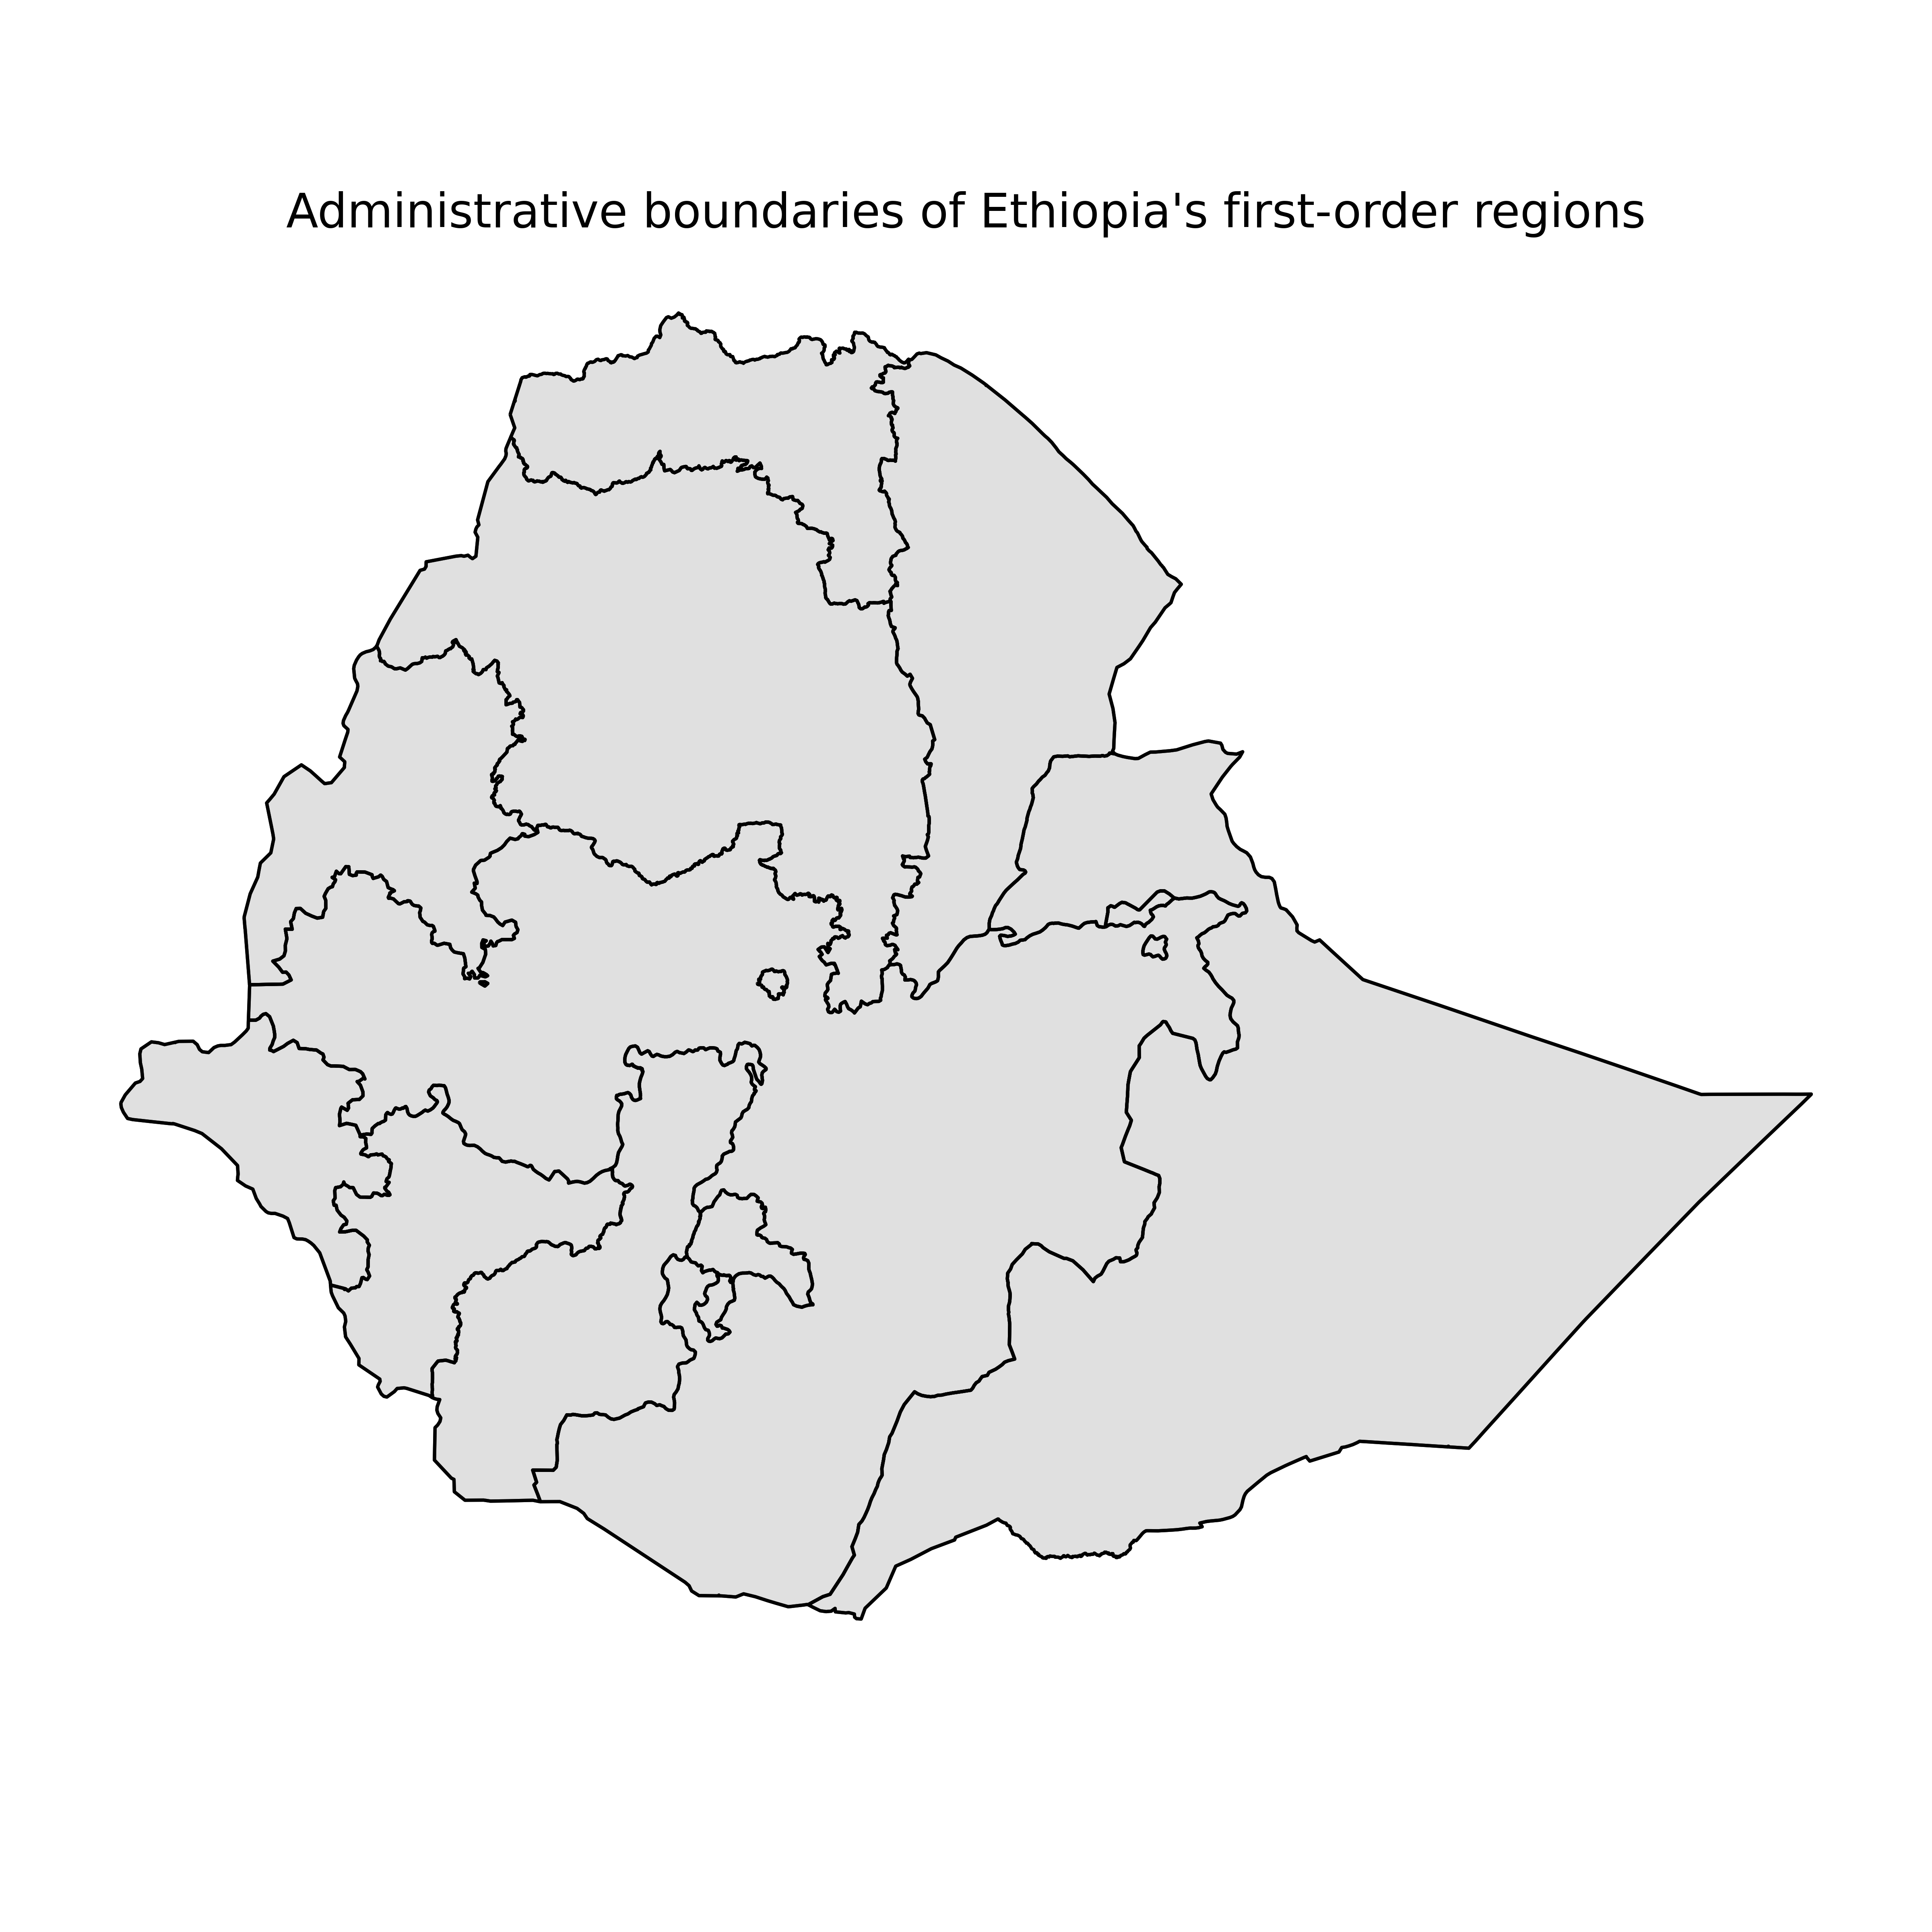
\includegraphics[width=0.7\textwidth]{outputs/figures/admin/ethiopia_admin_map.png}
	\caption{Administrative boundaries of Ethiopia's first-order regions. The map displays the 13 regional units used in the analysis, highlighting the evolving and fragmented nature of administrative boundaries over the study period.}
	\label{fig:admin_map}
\end{figure}
% --- End Figure 5 ---

\section{Identification Challenges in Small-N Panel Settings}

In empirical analyses of political favoritism using nighttime lights (NTL) data, identification is particularly challenging in settings with a small number of regions, limited exogenous variation in treatment, and high outcome concentration. This section outlines three core challenges that jointly limit inference in such panel data contexts.

\subsection{Omitted Variable Bias (without time fixed effects)}

When time fixed effects are omitted from panel regressions, estimates of leader-region favoritism are vulnerable to omitted variable bias. In the Ethiopian context, national economic shocks—such as booms or downturns—often coincide with leadership transitions. Without controlling for year effects, the estimated association between a leader’s birth region and regional luminosity may simply reflect these broader national trends, rather than any causal effect of political favoritism. Empirically, baseline models that exclude time fixed effects tend to produce inflated and statistically significant coefficients, but placebo tests and diagnostic plots reveal that these results are largely driven by common shocks rather than genuine treatment effects.

\subsection{Limited Identifying Variation (with time fixed effects)}

Including time fixed effects absorbs national shocks and common trends, but in small-N settings with few treated units and limited within-region, within-year variation, this approach introduces a new problem: limited identifying variation. When the timing of leader transitions is highly collinear with year effects, the model cannot reliably distinguish leader-region effects from national shocks. In the Ethiopian panel, the inclusion of time fixed effects sharply attenuates the estimated coefficients and increases standard errors, indicating that the available variation is insufficient for robust identification. The empirical p-values from placebo tests further confirm that observed effects are not distinguishable from random assignment.

\subsection{Low Statistical Power (small number of treated units)}

A third challenge is low statistical power, which arises from the small number of regions and limited number of leadership transitions. With only a handful of treated units and sparse treatment events, the effective sample size for identifying leader-region effects is severely constrained. This results in wide confidence intervals and imprecise estimates, particularly in event-study analyses and placebo simulations. The inability to detect dynamic effects or distinguish real from placebo results is a direct consequence of this low power, as demonstrated by the high empirical p-values and the overlap between observed and placebo distributions.

\paragraph{Synthesis}

Taken together, these challenges—omitted variable bias, limited identifying variation, and low statistical power—jointly undermine the credibility of causal inference in small-N panel settings. In the Ethiopian case, and in similar contexts, the combination of these factors means that apparent evidence for political favoritism is not empirically distinguishable from noise. Robust identification requires richer data, more exogenous variation, and careful diagnostic testing to avoid spurious findings.

\section{Literature Review}
This study sits at the intersection of three literatures.

First, a substantial literature uses satellite luminosity to measure economic activity. Early work established that light emissions track national and regional output surprisingly well in settings with limited conventional statistics \citep{Chen2011,Henderson2012}. More recent contributions show that the strength of this relationship varies with population density, sectoral composition, and spatial scale, which makes local interpretation more difficult than national validation exercises might suggest \citep{Bluhm2022,Gibson2021}. Work on harmonized long-run products has also improved the temporal comparability of DMSP-OLS and VIIRS series, but it has not eliminated measurement challenges \citep{Li2023,Gibson2024}.

Second, the paper relates to research on regional and ethnic favoritism. \citet{Hodler2014} show that political leaders' birth regions tend to receive higher nighttime light intensity in a broad cross-country sample. Subsequent work has refined that perspective by emphasizing the interaction between political favoritism, local ethnic demography, and institutions \citep{BeiserMcGrath2021}. Recent studies also continue to find geographically targeted favoritism in other settings, including public investment and local clientelism \citep{Onana2024,Cruzatti2024}. The implication is not that favoritism is universal, but that claims about it should be tested against within-unit changes rather than cross-sectional differences.




Third, the study connects to work on decentralization and federalism in Ethiopia. Existing scholarship highlights the tension between formal regional autonomy and persistent vertical control, including constraints on local fiscal autonomy and uneven developmental capacity \citep{Faguet2021,Wubneh2017}. Those institutional features make Ethiopia a theoretically important case for studying regional inequality, but they also heighten the need for careful empirical design. If regional trajectories differ for structural reasons unrelated to political leadership, pooled cross-sectional comparisons can easily be mistaken for favoritism.

\subsection*{Political Economy of Ethiopian Federalism}
The spatial distribution of rents in Ethiopia is deeply shaped by the country’s federal architecture and the political strategies of its ruling coalitions. Under the Ethiopian People’s Revolutionary Democratic Front (EPRDF), federalism was formally enshrined, but real power remained highly centralized. The EPRDF’s dominance over regional governments meant that resource allocation, investment, and development projects were often coordinated from the center, with regional administrations acting as agents rather than autonomous principals. This centralization is theorized to produce a spatial distribution of rents that is less responsive to local political dynamics and more reflective of national priorities and coalition management. In contrast, the current administration has presided over a period of greater regional contestation and, in some cases, increased regional autonomy. According to \citet{Faguet2021}, such shifts can alter the expected pattern of rent distribution: as regional governments gain more effective autonomy, the allocation of resources may become more sensitive to local political competition, ethnic demography, and the bargaining power of regional elites. This theoretical perspective suggests that the empirical analysis of favoritism in Ethiopia must account for changes in the structure of federalism and the evolving balance of power between center and regions.

Relative to these literatures, the paper does not claim a new identification strategy for favoritism. Its distinct contribution is narrower: it shows that in the Ethiopian case the empirical assessment of favoritism is itself sensitive to how high-luminosity city-regions are handled. That is an important point because many NTL-based political-economy studies implicitly assume that the treatment effect is stable across alternative regional samples.

\section{Methodology}
\subsection{Data}
\subsubsection{Nighttime light data}
The repository contains a harmonized annual NTL series built from DMSP-OLS and VIIRS raster products. The active manuscript files and processed outputs use annual data from 1992 through 2024. The underlying scripts reference the pixel-scale corrected nighttime light product of \citet{Li2023} and annual VIIRS composites derived by \citet{Elvidge2021}. Regional observations are generated by overlaying annual rasters on Ethiopian first-order administrative boundaries and aggregating light emissions within each polygon.

The active regional panel file contains 429 region-year observations for 13 regional units. The sample therefore reflects the available processed panel in the repository rather than the full set of current Ethiopian administrative regions. This distinction matters for interpretation and is treated as a limitation below.
% --- Begin Figure 5: Admin Map ---
\begin{figure}[ht]
	\centering
	% Replace the following line with the actual path to your admin map graphic
	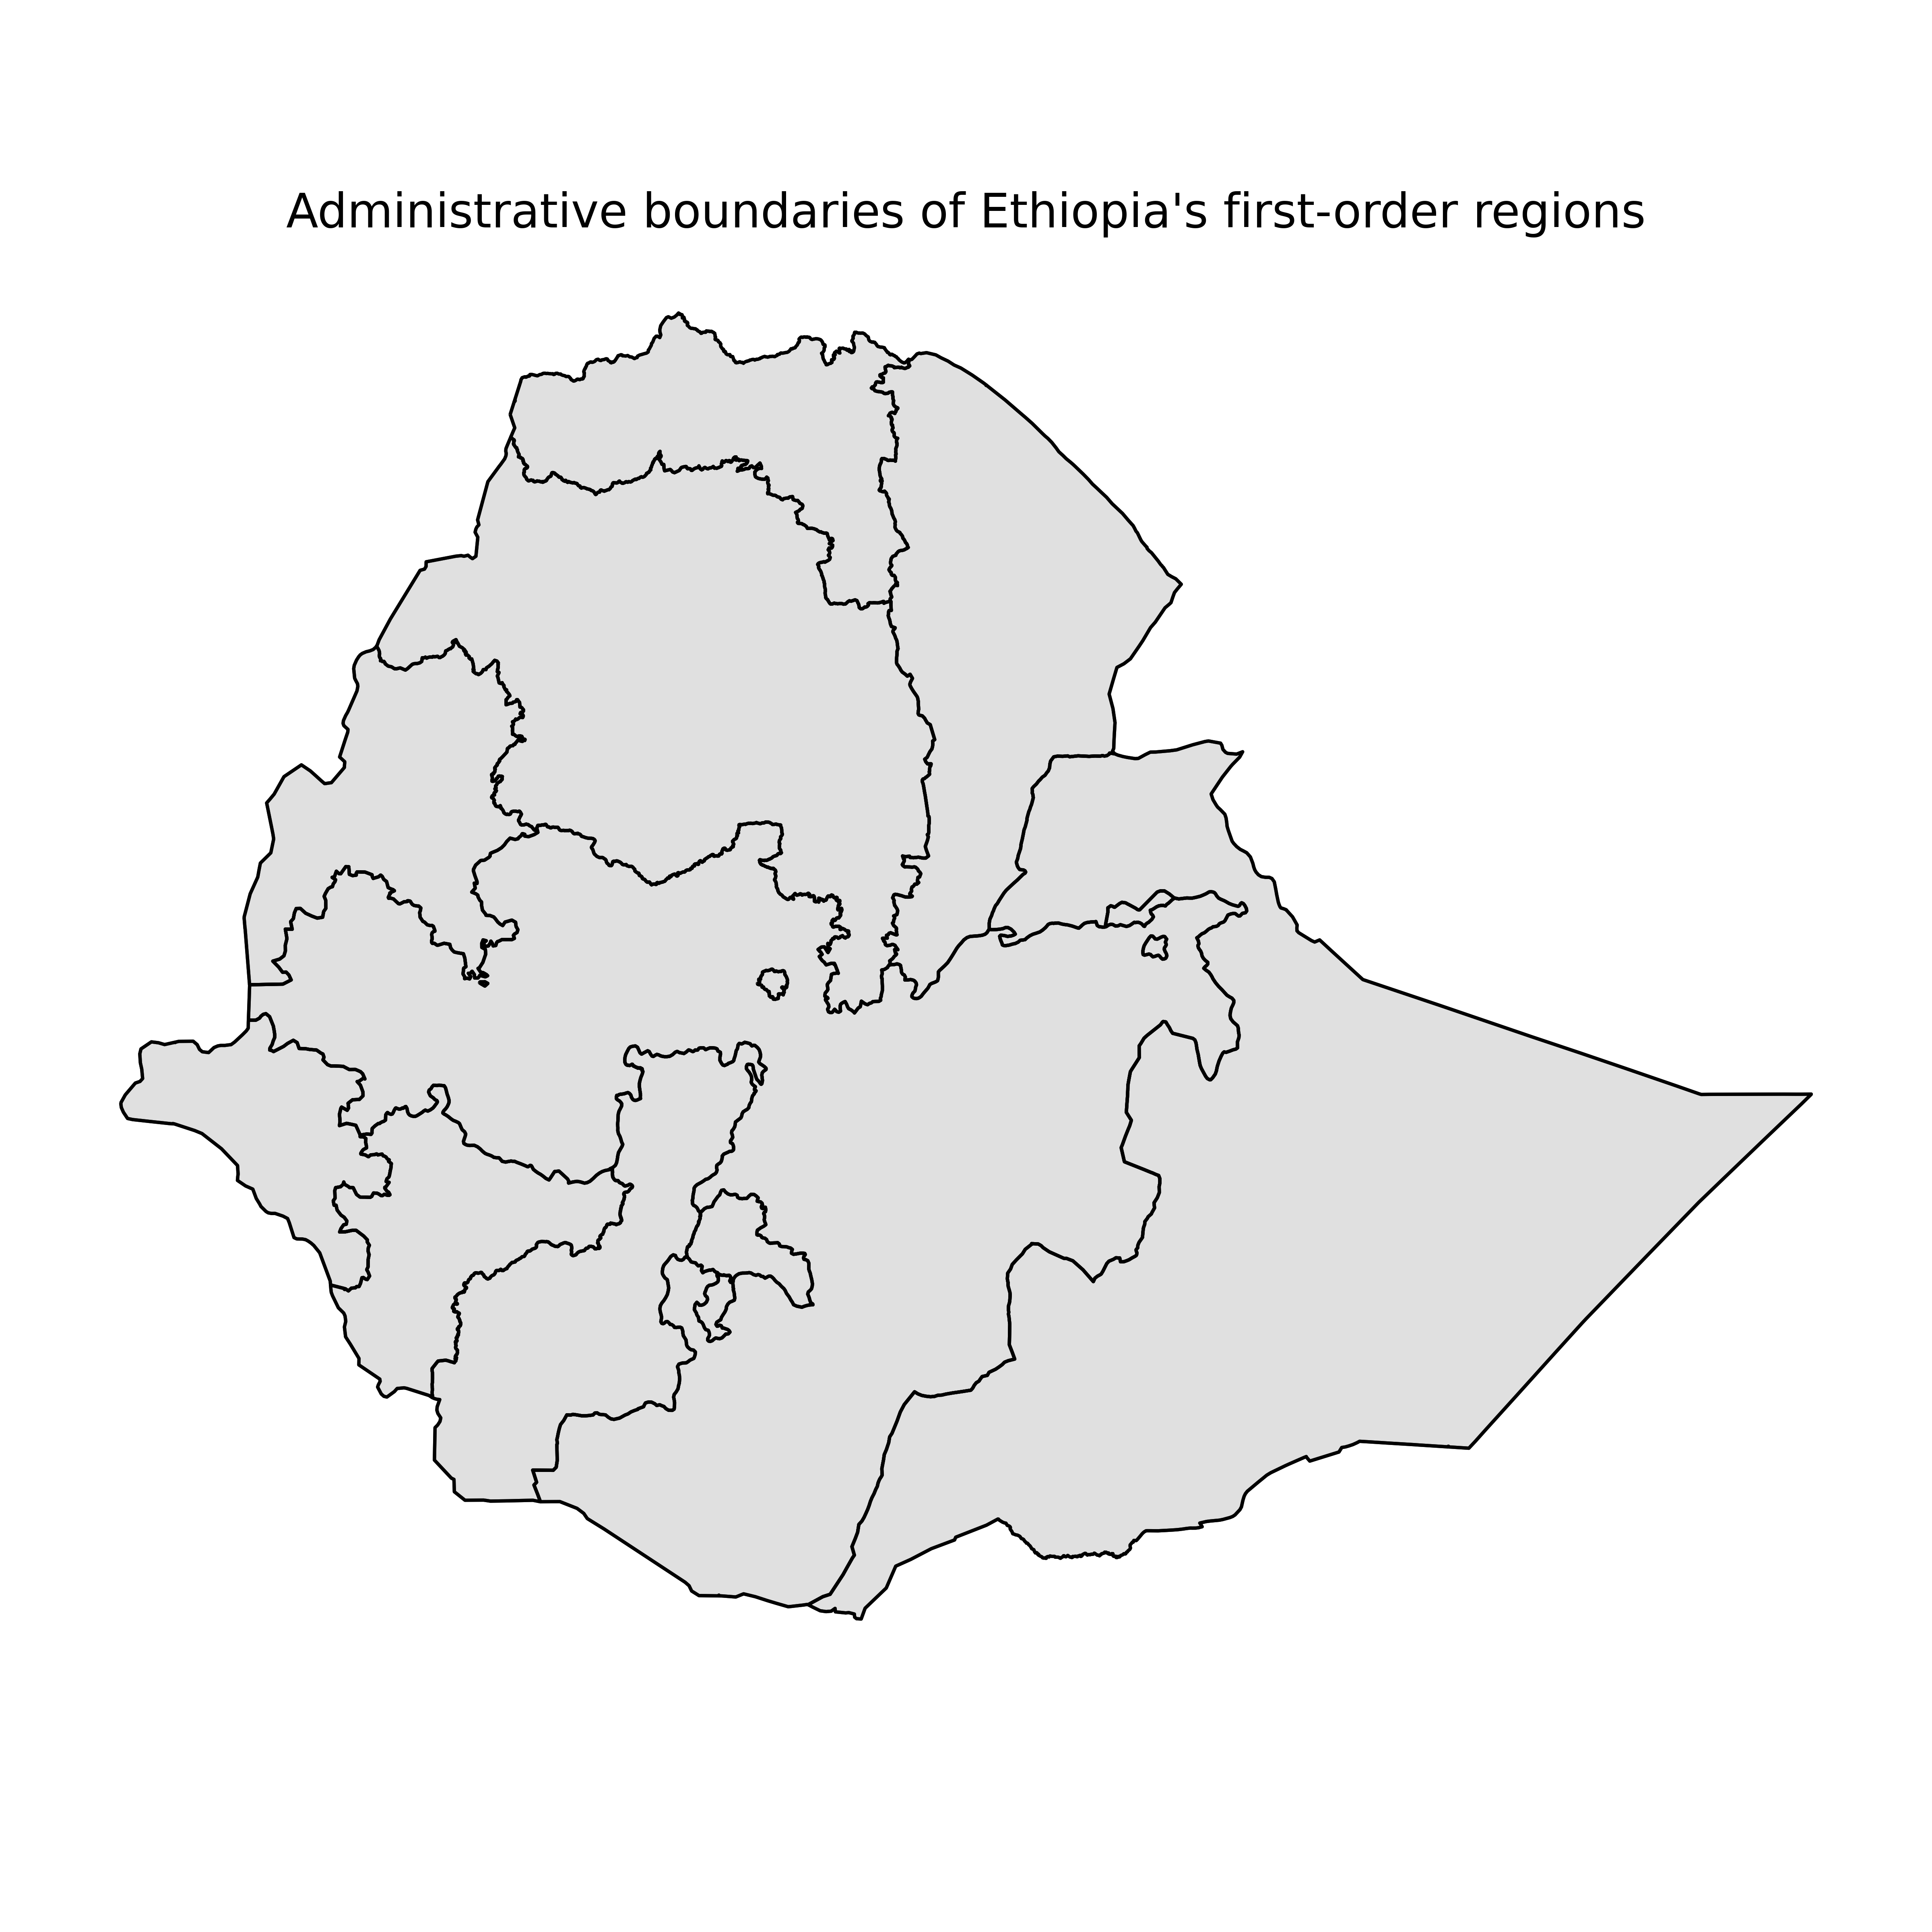
\includegraphics[width=0.7\textwidth]{outputs/figures/admin/ethiopia_admin_map.png}
	\caption{Administrative boundaries of Ethiopia's first-order regions. The map displays the 13 regional units used in the analysis, highlighting the evolving and fragmented nature of administrative boundaries over the study period.}
	\label{fig:admin_map}
\end{figure}
% --- End Figure 5 ---

\section{Identification Challenges in Small-N Panel Settings}

In empirical analyses of political favoritism using nighttime lights (NTL) data, identification is particularly challenging in settings with a small number of regions, limited exogenous variation in treatment, and high outcome concentration. This section outlines three core challenges that jointly limit inference in such panel data contexts.

\subsection{Omitted Variable Bias (without time fixed effects)}

When time fixed effects are omitted from panel regressions, estimates of leader-region favoritism are vulnerable to omitted variable bias. In the Ethiopian context, national economic shocks—such as booms or downturns—often coincide with leadership transitions. Without controlling for year effects, the estimated association between a leader’s birth region and regional luminosity may simply reflect these broader national trends, rather than any causal effect of political favoritism. Empirically, baseline models that exclude time fixed effects tend to produce inflated and statistically significant coefficients, but placebo tests and diagnostic plots reveal that these results are largely driven by common shocks rather than genuine treatment effects.

\subsection{Limited Identifying Variation (with time fixed effects)}

Including time fixed effects absorbs national shocks and common trends, but in small-N settings with few treated units and limited within-region, within-year variation, this approach introduces a new problem: limited identifying variation. When the timing of leader transitions is highly collinear with year effects, the model cannot reliably distinguish leader-region effects from national shocks. In the Ethiopian panel, the inclusion of time fixed effects sharply attenuates the estimated coefficients and increases standard errors, indicating that the available variation is insufficient for robust identification. The empirical p-values from placebo tests further confirm that observed effects are not distinguishable from random assignment.

\subsection{Low Statistical Power (small number of treated units)}

A third challenge is low statistical power, which arises from the small number of regions and limited number of leadership transitions. With only a handful of treated units and sparse treatment events, the effective sample size for identifying leader-region effects is severely constrained. This results in wide confidence intervals and imprecise estimates, particularly in event-study analyses and placebo simulations. The inability to detect dynamic effects or distinguish real from placebo results is a direct consequence of this low power, as demonstrated by the high empirical p-values and the overlap between observed and placebo distributions.

\paragraph{Synthesis}

Taken together, these challenges—omitted variable bias, limited identifying variation, and low statistical power—jointly undermine the credibility of causal inference in small-N panel settings. In the Ethiopian case, and in similar contexts, the combination of these factors means that apparent evidence for political favoritism is not empirically distinguishable from noise. Robust identification requires richer data, more exogenous variation, and careful diagnostic testing to avoid spurious findings.

\section{Literature Review}
This study sits at the intersection of three literatures.

First, a substantial literature uses satellite luminosity to measure economic activity. Early work established that light emissions track national and regional output surprisingly well in settings with limited conventional statistics \citep{Chen2011,Henderson2012}. More recent contributions show that the strength of this relationship varies with population density, sectoral composition, and spatial scale, which makes local interpretation more difficult than national validation exercises might suggest \citep{Bluhm2022,Gibson2021}. Work on harmonized long-run products has also improved the temporal comparability of DMSP-OLS and VIIRS series, but it has not eliminated measurement challenges \citep{Li2023,Gibson2024}.

Second, the paper relates to research on regional and ethnic favoritism. \citet{Hodler2014} show that political leaders' birth regions tend to receive higher nighttime light intensity in a broad cross-country sample. Subsequent work has refined that perspective by emphasizing the interaction between political favoritism, local ethnic demography, and institutions \citep{BeiserMcGrath2021}. Recent studies also continue to find geographically targeted favoritism in other settings, including public investment and local clientelism \citep{Onana2024,Cruzatti2024}. The implication is not that favoritism is universal, but that claims about it should be tested against within-unit changes rather than cross-sectional differences.




Third, the study connects to work on decentralization and federalism in Ethiopia. Existing scholarship highlights the tension between formal regional autonomy and persistent vertical control, including constraints on local fiscal autonomy and uneven developmental capacity \citep{Faguet2021,Wubneh2017}. Those institutional features make Ethiopia a theoretically important case for studying regional inequality, but they also heighten the need for careful empirical design. If regional trajectories differ for structural reasons unrelated to political leadership, pooled cross-sectional comparisons can easily be mistaken for favoritism.

\subsection*{Political Economy of Ethiopian Federalism}
The spatial distribution of rents in Ethiopia is deeply shaped by the country’s federal architecture and the political strategies of its ruling coalitions. Under the Ethiopian People’s Revolutionary Democratic Front (EPRDF), federalism was formally enshrined, but real power remained highly centralized. The EPRDF’s dominance over regional governments meant that resource allocation, investment, and development projects were often coordinated from the center, with regional administrations acting as agents rather than autonomous principals. This centralization is theorized to produce a spatial distribution of rents that is less responsive to local political dynamics and more reflective of national priorities and coalition management. In contrast, the current administration has presided over a period of greater regional contestation and, in some cases, increased regional autonomy. According to \citet{Faguet2021}, such shifts can alter the expected pattern of rent distribution: as regional governments gain more effective autonomy, the allocation of resources may become more sensitive to local political competition, ethnic demography, and the bargaining power of regional elites. This theoretical perspective suggests that the empirical analysis of favoritism in Ethiopia must account for changes in the structure of federalism and the evolving balance of power between center and regions.

Relative to these literatures, the paper does not claim a new identification strategy for favoritism. Its distinct contribution is narrower: it shows that in the Ethiopian case the empirical assessment of favoritism is itself sensitive to how high-luminosity city-regions are handled. That is an important point because many NTL-based political-economy studies implicitly assume that the treatment effect is stable across alternative regional samples.

\section{Methodology}
\subsection{Data}
\subsubsection{Nighttime light data}
The repository contains a harmonized annual NTL series built from DMSP-OLS and VIIRS raster products. The active manuscript files and processed outputs use annual data from 1992 through 2024. The underlying scripts reference the pixel-scale corrected nighttime light product of \citet{Li2023} and annual VIIRS composites derived by \citet{Elvidge2021}. Regional observations are generated by overlaying annual rasters on Ethiopian first-order administrative boundaries